\documentclass[12pt]{article}

\usepackage[margin=1in,footskip=0.25in]{geometry}
\usepackage{amsmath}
\usepackage{amssymb}
\usepackage{graphicx}
\usepackage{hyperref}
\usepackage{makeidx}
\usepackage{listings}
\usepackage{minted}
\usemintedstyle{friendly}

\setcounter{tocdepth}{2}

\hypersetup{
    colorlinks=true,
    linkcolor=blue,       % Color for internal links
    urlcolor=blue         % Color for external URLs
}

% Number equations, figures, and tables within sections
\numberwithin{equation}{section}
\numberwithin{figure}{section}
\numberwithin{table}{section}

\makeindex

\begin{document}

\title{Fluid Mechanics for Ocean Scientists}
\author{Milan Curcic}
\date{}

\maketitle

\tableofcontents

\newpage
\section{Introduction}

\subsection{What will you learn in this course}

The course aims to provide students with a solid understanding of key fluid
mechanics concepts that are used in ocean physics research.
This course will first refresh you on the vector calculus needed to understand
fluid mechanics, and introduce the Eulerian and Lagrangian views of the flow.
We then proceed to derive the conservation equations for mass and momentum.
We will then consider the effects of rotation and stratification, and look
at some steady solutions of the rotating Navier-Stokes equations.
Then, we will simplify the flow by looking at it as a thin layer of
incompressible rotating fluid that flows over a variable bottom topography
and a free surface.
From there, we will study turbulence and boundary layers, and complete the
course with the linear theory of surface gravity waves.
By the end of the course, you will be proficient in applying fluid mechanical
concepts and mathematical tools to solve many ocean physics research problems.
It will also prepare you for more specialized courses on turbulence, waves,
and geophysical fluid dynamics.

\subsection{Reference textbooks}

These lecture notes are based on the following textbooks:

\begin{enumerate}
  \item \textit{Fluid Mechanics}, 6th Ed., by Kundu, Cohen, and Dowling (Elsevier);
  \item \textit{Atmospheric and Oceanic Fluid Dynamics} (AOFD) by Geoffrey Vallis (Cambridge University Press);
  \item \textit{Turbulent Flows} by Stephen Pope (Cambridge University Press);
  \item \textit{Water Wave Mechanics for Engineers and Scientists} by Dean and Dalrymple (World Scientific).
\end{enumerate}

While the notes contain the distilled and required information for you to
succeed in this course, please refer to these textbooks for more detailed
explanations and examples.

\newpage
\section{Review of vector calculus}

In this section we will review the necessary concepts from vector calculus that
we will use in this course.
These include:
scalars, vectors and tensors;
gradient, divergence, and curl;
line, surface, and volume integrals;
and the Gauss and Stokes theorems.

\subsection{Scalars, vectors, and tensors}

In this course we will mainly use three types of quantities to describe fluid
properties: \textit{scalars}, \textit{vectors}, and \textit{tensors}.

\textit{Scalars}\index{Scalar} are completely described by their magnitude.
Examples of scalars are temperature, pressure, or density.
A value of 290 K, for example, completely describes the temperature of a fluid
at some point in space and time.
We will write them in equations using italics, e.g. $T$, $p$, $\rho$.

\textit{Vectors}\index{Vector} have both magnitude and direction.
Examples of vector are velocity, acceleration, or force.
In 3-dimensional Cartesian space with coordinates $(x, y, z)$, for example,
vector $\mathbf{u}(x,y,z)$ can be described by its components

\begin{equation}
  \mathbf{u} =
  \begin{bmatrix}
    u_x \\
    u_y \\
    u_z
  \end{bmatrix}
\end{equation}
where $u_x$, $u_y$, and $u_z$ (each a scalar) are the components of $\mathbf{u}$
in the $x$, $y$, and $z$ directions, respectively.
This is the conventional notation, however, we will often write vectors
inline as $\mathbf{u} = (u_x, u_y, u_z)$.
We will write vectors in equations using boldface, e.g. $\mathbf{u}$,
$\mathbf{a}$, or $\mathbf{F}$.

The magnitude\index{Vector!magnitude}, or norm\index{Vector!norm}, of a 
$\mathbf{u}$ is denoted by $||\mathbf{u}||$, and is calculated as

\begin{equation}
  ||\mathbf{u}|| = \sqrt{u_x^2 + u_y^2 + u_z^2}
\end{equation}

\textit{Tensors}\index{Tensor} have magnitude, direction, and orientation, such as stress or
strain.
They are vectors that act on each respective surface orthogonal to the direction
of the tensor.
In 3-dimensional space, for example, a stress tensor can be described as:

\begin{equation}
  \boldsymbol{\tau} =
  \begin{bmatrix}
    \tau_{xx} & \tau_{xy} & \tau_{xz} \\
    \tau_{yx} & \tau_{yy} & \tau_{yz} \\
    \tau_{zx} & \tau_{zy} & \tau_{zz}
  \end{bmatrix}
\end{equation}
In this notation and index ordering, i.e. $\tau_{ij}$, the first index ($i$)
refers to the direction of the stress component, and the second index ($j$)
refers to the direction of the normal to the surface.
In other words, each row of the tensor contains the three components of a
vector, and each column contains the three surface normals that the stress
component is acting on.
For example, $\tau_{xy}$ is the stress in the x-direction and is acting on the
surface whose normal is in the y-direction (and which lies in the x-z plane).

One special type of tensor is the \textit{identity tensor}\index{Tensor!identity}
$\mathbf{I}$, which is a tensor that maps a vector onto itself.
In Cartesian coordinates, it is given by:

\begin{equation}
  \mathbf{I} =
  \begin{bmatrix}
    1 & 0 & 0 \\
    0 & 1 & 0 \\
    0 & 0 & 1
  \end{bmatrix}
\end{equation}

It may be useful to think of scalars as 0$^{th}$-order tensors, vectors as
1$^{st}$-order tensors, and tensors as 2$^{nd}$-order tensors.\\

\subsection{Unit vectors}

Unit vectors\index{Vector!unit} are vectors with magnitude of 1.
A popular notation for unit vectors in Cartesian coordinates is $\mathbf{i}$,
$\mathbf{j}$, and $\mathbf{k}$, which point in the $x$, $y$, and $z$ directions,
respectively.
So, a vector $\mathbf{u}$ can be written as

\begin{equation}
  \mathbf{u} = u_x \mathbf{i} + u_y \mathbf{j} + u_z \mathbf{k}
\end{equation}

Notice that you can get get the unit vector by dividing any vector by its
magnitude, i.e. $\mathbf{u}/||u||$.

\subsection{Vector operations}

Two vectors can be added, subtracted, or multiplied.
Although vector addition and subtraction are straightforward, vector
multiplication is more interesting.
There are two types of vector multiplication: the \textit{dot product} and the
\textit{cross product}.

\subsubsection{Dot product}

The dot product\index{Product!dot} of two 3-dimensional Cartesian vectors
$\mathbf{a}$ and $\mathbf{b}$ is an element-wise sum of their components
(and thus, a scalar!):

\begin{equation}
  \mathbf{a} \cdot \mathbf{b} =
  \begin{bmatrix}
    a_1 \\
    a_2 \\
    a_3
  \end{bmatrix}
  \cdot
  \begin{bmatrix}
    b_1 \\
    b_2 \\
    b_3
  \end{bmatrix}
  = a_1 b_1 + a_2 b_2 + a_3 b_3
\end{equation}

More generally, the dot product of two n-dimensional vectors $\mathbf{a}$ and
$\mathbf{b}$ is

\begin{equation}
  \mathbf{a} \cdot \mathbf{b} = \sum_{i=1}^{n} a_i b_i = a_1 b_1 + a_2 b_2 + \ldots + a_n b_n
\end{equation}

The dot product is commutative, meaning that
$\mathbf{a} \cdot \mathbf{b} = \mathbf{b} \cdot \mathbf{a}$.

The magnitude of a dot product of two vectors is equal to the product of their
magnitudes and the cosine of the angle $\theta$ between them:

\begin{equation}
  \mathbf{a} \cdot \mathbf{b} = ||\mathbf{a}|| ||\mathbf{b}|| \cos{\theta}
\end{equation}
To visualize this relationship, take one vector and project it onto the other.
This projection is the magnitude of the vector times the cosine of the angle
between them.
Now one vector and the projection of the other onto the first vector are
pointing in the same direction, so their dot product is the product of their
magnitudes.
It can be useful to think of a dot product as collapsing the two vectors into a
single number contains contributions from each of their components.

The following listing shows how to compute the dot product of two vectors
in Python using the built-in arithmetic operators.

\begin{listing}[h]
\begin{minted}[numbersep=5pt, frame=lines, framesep=2mm]{python}
import numpy as np

# initialize two vectors; specific values are arbitrary.
a = np.array([1, 2, 3])
b = np.array([4, 5, 6])

c = 0  # initialize the result variable
for i in range(a.size):  # loop over indices of the vector
    c += a[i] * b[i]  # multiply elements and add to the result
\end{minted}
\label{lst:dot_product_arithmetic}
\end{listing}
The NumPy library, however, allows element-wise multiplication of vectors,
which is both more efficient and more concise:

\begin{listing}[h]
\begin{minted}[numbersep=5pt, frame=lines, framesep=2mm]{python}
c = np.sum(a * b)  # multiply element-wise and sum up the components
\end{minted}
\label{lst:dot_product_numpy}
\end{listing}
Even though the dot product is simple to implement, as we did above, NumPy
provides a function that is even more concise, and likely the most efficient
way to compute the dot product:

\begin{listing}[h]
\begin{minted}[numbersep=5pt, frame=lines, framesep=2mm]{python}
c = np.dot(a, b)
\end{minted}
\label{lst:dot_product_numpy_dot}
\end{listing}
Although it's important to understand how to implement the fundamental vector
operations by hand, and do it yourself at least once, in practice it's best to
use established libraries such as NumPy, as they are well tested and optimized
for computational efficiency.

\subsubsection{Cross product}

The cross product\index{Product!cross} of two vectors $\mathbf{a}$ and
$\mathbf{b}$ is defined as:

\begin{equation}
  \mathbf{a} \times \mathbf{b} =
  det \begin{bmatrix}
    \mathbf{i} & \mathbf{j} & \mathbf{k} \\
    a_x & a_y & a_z \\
    b_x & b_y & b_z
  \end{bmatrix}
\end{equation}
where $det(\mathbf{M})$ means the \textit{determinant of matrix $\mathbf{M}$}.

Using the so-called \textit{rule of Sarrus}, the cross product can be calculated
as:

\begin{equation}
  \mathbf{a} \times \mathbf{b} = (a_y b_z - a_z b_y) \mathbf{i} +
    (a_z b_x - a_x b_z) \mathbf{j} + (a_x b_y - a_y b_x) \mathbf{k}
\end{equation}
or:

\begin{equation}
  \mathbf{a} \times \mathbf{b} =
    \begin{bmatrix}
      a_y b_z - a_z b_y \\
      a_z b_x - a_x b_z \\
      a_x b_y - a_y b_x
    \end{bmatrix}
\end{equation}

The result of a cross product is a vector that is orthogonal to both $\mathbf{a}$
and $\mathbf{b}$.
Its orientation in space is determined by the right-hand rule:
if you point your right thumb in the direction of $\mathbf{a}$ and your index
finger in the direction of $\mathbf{b}$, then your middle finger will point in
the direction of $\mathbf{a} \times \mathbf{b}$.

The magnitude of the cross product is equal to the product of the magnitudes of
the two vectors times the sine of the angle between them:

\begin{equation}
  ||\mathbf{a} \times \mathbf{b}|| = ||\mathbf{a}|| ||\mathbf{b}|| \sin{\theta}
  \label{eq:cross_product_magnitude}
\end{equation}
So, the magnitude of the cross product is largest when the two vectors are
orthogonal.

Unlike the dot product, the cross product is anticommutative, meaning that
$\mathbf{a} \times \mathbf{b} = -\mathbf{b} \times \mathbf{a}$.

In fluid mechanics a cross product will often come up when we are interested in
the rotation of a vector field, such as vorticity.

\subsection{Matrix multiplication}

Occasionally, we will need to multiply a vector by a matrix, or, a matrix by a
matrix.
As a vector is a special case of a matrix in which either the number of rows or
columns is 1, the same rules of matrix multiplication will apply when we
multiply a vector by a matrix or a matrix by a matrix.
These operations are not commutative, meaning that the order of multiplication
matters.

Take two matrices $\mathbf{A}$ and $\mathbf{B}$ such that

\begin{equation}
  \mathbf{A} =
  \begin{bmatrix}
    a_{11} & a_{12} & a_{13} \\
    a_{21} & a_{22} & a_{23} \\
    a_{31} & a_{32} & a_{33}
  \end{bmatrix}
\end{equation}
and:

\begin{equation}
  \mathbf{B} =
  \begin{bmatrix}
    b_{11} & b_{12} & b_{13} \\
    b_{21} & b_{22} & b_{23} \\
    b_{31} & b_{32} & b_{33}
  \end{bmatrix}
\end{equation}

The result of their multiplication is a matrix $\mathbf{C}$ given by:

\begin{equation}
  \mathbf{C} = \mathbf{A} \mathbf{B} =
  \begin{bmatrix}
    a_{11} b_{11} + a_{12} b_{21} + a_{13} b_{31} &
    a_{11} b_{12} + a_{12} b_{22} + a_{13} b_{32} &
    a_{11} b_{13} + a_{12} b_{23} + a_{13} b_{33} \\
    a_{21} b_{11} + a_{22} b_{21} + a_{23} b_{31} &
    a_{21} b_{12} + a_{22} b_{22} + a_{23} b_{32} &
    a_{21} b_{13} + a_{22} b_{23} + a_{23} b_{33} \\
    a_{31} b_{11} + a_{32} b_{21} + a_{33} b_{31} &
    a_{31} b_{12} + a_{32} b_{22} + a_{33} b_{32} &
    a_{31} b_{13} + a_{32} b_{23} + a_{33} b_{33}
  \end{bmatrix}
\end{equation}

That is, the entry $c_{ij}$ of the product is obtained by multiplying
term-by-term the entries of the $i$-th row of $\mathbf{A}$ and the $j$-th column
of $\mathbf{B}$, and summing these products.
In other words, $c_{ij}$ is the dot product of the $i$-th row of $\mathbf{A}$
and the $j$-th column of $\mathbf{B}$.

\subsection{Total and partial derivatives}

We will denote total\index{Derivative!total} and partial\index{Derivative!partial}
derivative operators (for example, in time $t$)
as $\frac{d}{dt}$ and $\frac{\partial}{\partial t}$.
Scalars, vectors, and tensors alike can be differentiated with respect to any
variable.
A derivative of a vector is simply a vector of derivatives of its components:

\begin{equation}
  \frac{d\mathbf{u}}{dt}
    = (\frac{d u_x}{d t}, \frac{d u_y}{d t}, \frac{d u_z}{d t})
    = \frac{du_x}{dt} \mathbf{i} + \frac{du_y}{dt} \mathbf{j} + \frac{du_z}{dt} \mathbf{k}
    = \begin{bmatrix}
        \frac{du_x}{dt} \\
        \frac{du_y}{dt} \\
        \frac{du_z}{dt}
      \end{bmatrix}
\end{equation}

\begin{equation}
  \frac{\partial \mathbf{u}}{\partial t}
    = (\frac{\partial u_x}{\partial t}, \frac{\partial u_y}{\partial t}, \frac{\partial u_z}{\partial t})
    = \frac{\partial u_x}{\partial t} \mathbf{i} + \frac{\partial u_y}{\partial t} \mathbf{j} + \frac{\partial u_z}{\partial t} \mathbf{k}
    = \begin{bmatrix}
        \frac{\partial u_x}{\partial t} \\
        \frac{\partial u_y}{\partial t} \\
        \frac{\partial u_z}{\partial t}
      \end{bmatrix}
\end{equation}
and likewise for tensors.\\

\subsection{Gradient, divergence, and curl}

Now, we introduce another new operator that builds on top of previous
concepts to describe how scalar and vector fields change in space.
This operator is called \textit{del}\index{Del} and is denoted by the symbol
$\nabla$\index{Nabla} (pronounced "nabla"):

\begin{equation}
  \label{eq:nabla}
  \nabla = \frac{\partial}{\partial x} \mathbf{i} +
    \frac{\partial}{\partial y} \mathbf{j} +
    \frac{\partial}{\partial z} \mathbf{k}
\end{equation}

A good way to think about $\nabla$ is as of a \textit{differential operator},
which itself is a 3-dimensional vector that can operate on scalars or vectors.
Specifically:

\begin{itemize}
  \item $\nabla p$ is as vector that is a gradient of a scalar field $p$;
  it quantifies how $p$ changes in space.
  \item $\nabla \cdot \mathbf{u}$ is a scalar that is the divergence of a vector
  field $\mathbf{u}$; it quantifies how $\mathbf{u}$ flows out of a point.
  \item $\nabla \times \mathbf{u}$ is a vector that is the curl of a vector field
  $\mathbf{u}$; it quantifies how $\mathbf{u}$ rotates around a point.
\end{itemize}

Although, strictly speaking, one is a symbol and the other is an operator,
$\nabla$ ("nabla") and "del" are often used interchangeably.

\subsubsection{Gradient}

The gradient\index{Gradient} of a scalar field $T$ is a vector field that points in the
direction of the greatest rate of increase of $T$.
It is denoted by $\nabla T$ and is defined as

\begin{equation}
  \nabla T = \frac{\partial T}{\partial x} \mathbf{i} +
    \frac{\partial T}{\partial y} \mathbf{j} +
    \frac{\partial T}{\partial z} \mathbf{k}
\end{equation}

Gradient of a scalar field is a vector that points in the direction of the
steepest increase of that field, and its magnitude is the rate of that increase.
For example, imagine hiking up a hill; the gradient of the terrain is a vector
that is pointing toward the steepest incline, and its magnitude is the slope
of that incline.

\subsubsection{Divergence}

The divergence\index{Divergence} of a vector field $\mathbf{u}$ is a scalar field that describes
the rate at which the vector field flows out of a point.
It is denoted by $\nabla \cdot \mathbf{u}$ and is defined as

\begin{equation}
  \label{eq:divergence}
  \nabla \cdot \mathbf{u} = \frac{\partial u_x}{\partial x} +
    \frac{\partial u_y}{\partial y} + \frac{\partial u_z}{\partial z}
\end{equation}

Divergence of a vector field is a scalar that describes how much the vector
field is expanding or contracting at a point.
When divergence is negative, it is commonly referred to as convergence.

\subsubsection{Curl}

The curl\index{Curl} of a vector field $\mathbf{u}$ is a vector field that describes the
rotation of the vector field.
It is denoted by $\nabla \times \mathbf{u}$ and is defined as

\begin{equation}
  \nabla \times \mathbf{u} = \left( \frac{\partial u_z}{\partial y} -
    \frac{\partial u_y}{\partial z} \right) \mathbf{i} +
    \left( \frac{\partial u_x}{\partial z} -
    \frac{\partial u_z}{\partial x} \right) \mathbf{j} +
    \left( \frac{\partial u_y}{\partial x} -
    \frac{\partial u_x}{\partial y} \right) \mathbf{k}
\end{equation}

Curl of a vector field is another vector that is orthogonal to the original
vector field and quantifies how much the vector field is rotating around a
point.
When curl is zero, the vector field is said to be \textit{irrotational}.

\subsubsection{Useful vector identities}

Curl of a gradient of a scalar field is always zero:

\begin{equation}
  \nabla \times (\nabla T) = 0
\end{equation}
Further, divergence of a curl of a vector field is always zero:

\begin{equation}
  \nabla \cdot (\nabla \times \mathbf{u}) = 0
\end{equation}
Finally, curl of a curl of a vector field is:

\begin{equation}
  \nabla \times (\nabla \times \mathbf{u}) = \nabla (\nabla \cdot \mathbf{u}) - \nabla^2 \mathbf{u}
\end{equation}

Some of these identities will come handy when we derive the conservation of
vorticity laws.

\subsection{Gauss and Stokes theorems}

The most useful in our work will be variants of the
\textit{Gauss and Stokes theorems}.
The Gauss theorem relates a volume integral of a divergence of a vector field
to a surface integral of that vector field.
The Stokes theorem relates a surface integral of the curl of a vector field to
a line integral of that vector field.
Here, these are merely stated for reference.
We will explore their meaning and application in more detail as we use them
to derive the fundamental equations for fluid flows.

\subsubsection{Gauss theorem}

The Gauss theorem\index{Theorem!Gauss} states that the volume integral of the
divergence of a vector field $\mathbf{u}$ over a volume $V$ is equal to the
surface integral of $\mathbf{u}$ over the surface $A$ that encloses $V$:

\begin{equation}
  \label{eq:divergence_theorem}
  \int_V \nabla \cdot \mathbf{u} dV = \oint_A \mathbf{u} \cdot d\mathbf{A}
\end{equation}

This form of Gauss's theorem is also known as the
\textit{divergence theorem}\index{Theorem!divergence}.
It will come in handy when we derive the conservation of mass (continuity)
equation.

\subsubsection{Stokes theorem}

The Stokes theorem\index{Theorem!Stokes} states that the surface integral of the curl of a
vector field $\mathbf{u}$ over a surface $A$ is equal to the line integral of
$\mathbf{u}$ over the boundary of $A$:

\begin{equation}
  \int_A (\nabla \times \mathbf{u}) \cdot d\mathbf{A} = \oint_{\partial A} \mathbf{u} \cdot d\mathbf{l}
\end{equation}

\subsection{Summary}

In this chapter, we reviewed:

\begin{itemize}
  \item Scalars, vectors, and tensors;
  \item Vector algebra: dot product ($\mathbf{a} \cdot \mathbf{b}$) and cross
  product ($\mathbf{a} \times \mathbf{b}$);
  \item Derivatives: total ($\frac{d}{dt}$) and partial ($\frac{\partial}{\partial t}$);
  \item Gradient, divergence ($\nabla \cdot \mathbf{u}$), and curl ($\nabla \times \mathbf{u}$);
  \item Gauss theorem that relates volume and surface integrals:
  $\int_V \nabla \cdot \mathbf{u} dV = \oint_A \mathbf{u} \cdot d\mathbf{A}$;
  \item Stokes theorem that relates surface and line integrals:
  $\int_A (\nabla \times \mathbf{u}) \cdot d\mathbf{A} = \oint_{\partial A} \mathbf{u} \cdot d\mathbf{l}$.
\end{itemize}

These concepts will serve as the basic building blocks for everything that
follows in the remainder of this course.

\subsection{Exercises}

\begin{enumerate}
  
  \item Pick your favorite programming language (or ask for a recommendation for one).
  Write a program that defines a scalar, a vector, and a tensor, and assign
  numerical values to them.
  Print the values to the screen.
  Is there a difference in how you define them in your program?

  \item What is the dot product of two orthogonal vectors?
  How about the dot product of a vector with itself?
  Please write out the solution step by step.

  \item Write a program that calculates the cross product of two vectors.
  Please implement your solution using the basic arithmetic operations such as
  addition and multiplication.
  Then, see if your programming language or one of its software libraries
  provides a function to do this.
  Can you verify your implementation by comparing its output to that of the
  library function?

  \item How would you calculate a derivative of a quantity
  (scalar, for example) in a computer program, e.g. $\frac{\partial a}{\partial x}$?
  Consider that you can approximate a derivative as a difference between two
  values of the quantity at two points in space.
  In other words, assume $\partial a \approx \Delta a = a(x_2) - a(x_1)$,
  and similar for $x$.

  \item Write a computer program that calculates the gradient of a scalar field,
  and the divergence and curl of a vector field.
  
  \item Draw example vector fields that are: (a) non-divergent and irrotational,
  (b) divergent and irrotational, (c) non-divergent and rotational, and (d)
  divergent and rotational.
\end{enumerate}

\subsection*{Further reading}

\begin{itemize}
  \item Chapter 2 of \textit{Fluid Mechanics} by Kundu, Cohen, and Dowling
\end{itemize}

\newpage
\section{Fluid kinematics}

Fluid kinematics describe the fluid motion without considering the forces that
cause it.
We will explore two main views of the flow: the \textit{Lagrangian}\index{Lagrangian}
view, which follows individual fluid particles, and the \textit{Eulerian}\index{Eulerian}
view, which observes the flow at fixed points in space.
Although the Eulerian view is more commonly used in the theory and simulation
of fluid flows, the Lagrangian view will be essential in deriving some of the
fundamental equations, as well as for understanding where certain features of
the flow come from.
We will also introduce some useful concepts to describe the flow, namely
the \textit{velocity potential} and the \textit{stream function}.
These two scalar quantities are complementary to the vector field of velocity
and together provide a complete description of the flow.

\subsection{Lagrangian and Eulerian derivatives of a fluid property}

Consider a 3-dimensional quantity $\varphi$ that varies in space and time such that
$\varphi = \varphi(x, y, z, t)$.
Let's find the rate of change of $\varphi$.
Since it depends on $x$, $y$, $z$, and $t$, the rate of change of $\varphi$ along
each of these dimensions must be considered.
So, the total change of $\varphi$ (let's call it $\delta\varphi$) over spatial and
temporal increments $\delta x$, $\delta y$, $\delta z$, and $\delta t$ is the
sum of changes along each of these dimensions:

\begin{equation}
  \delta\varphi = \frac{\partial \varphi}{\partial x} \delta x +
    \frac{\partial \varphi}{\partial y} \delta y +
    \frac{\partial \varphi}{\partial z} \delta z +
    \frac{\partial \varphi}{\partial t} \delta t
\end{equation}
Divide by $\delta t$ to obtain:

\begin{equation}
  \frac{\delta\varphi}{\delta t} = \frac{\partial \varphi}{\partial x} \frac{\delta x}{\delta t} +
    \frac{\partial \varphi}{\partial y} \frac{\delta y}{\delta t} +
    \frac{\partial \varphi}{\partial z} \frac{\delta z}{\delta t} +
    \frac{\partial \varphi}{\partial t}
\end{equation}
Recall the definition of $\nabla$ (Eq. \ref{eq:nabla}), and let the finite
increment $\delta t$ approach $dt$ (and likewise for $\delta x$, $\delta y$, and
$\delta z$), to obtain:

\begin{equation}
  \frac{d\varphi}{dt} = \frac{\partial \varphi}{\partial x} \frac{dx}{dt} +
    \frac{\partial \varphi}{\partial y} \frac{dy}{dt} +
    \frac{\partial \varphi}{\partial z} \frac{dz}{dt} +
    \frac{\partial \varphi}{\partial t}
\end{equation}
Then, recognize that the velocity in each direction is the rate of change of
the position in that direction:

\begin{equation}
  \frac{d\varphi}{dt} =
    \frac{\partial \varphi}{\partial t} +
    u \frac{\partial \varphi}{\partial x} +
    v \frac{\partial \varphi}{\partial y} +
    w \frac{\partial \varphi}{\partial z} w
\end{equation}
Finally, recall the definition of $\nabla$ (Eq. \ref{eq:nabla}) to obtain:

\begin{equation}
  \label{eq:lagrangian_derivative}
  \frac{d\varphi}{dt} = \frac{\partial \varphi}{\partial t} + \mathbf{u} \cdot \nabla \varphi
\end{equation}
The term $\frac{d\varphi}{dt}$ is called the \textit{total derivative}\index{Derivative!total}
of $\varphi$. It is also called a \textit{Lagrangian derivative}\index{Derivative!Lagrangian},
or \textit{material derivative}\index{Derivative!material}, since it follows
the motion of a fluid particle.
The term $\frac{\partial \varphi}{\partial t}$ is called the
\textit{Eulerian derivative}\index{Derivative!Eulerian},
or \textit{partial derivative}\index{Derivative!partial}
of $\varphi$ with respect to time.
The term $\mathbf{u} \cdot \nabla \varphi$ describes how $\varphi$ changes due
to its spatial variation and the flow of the fluid.

Although the term $\mathbf{u} \cdot \nabla \varphi$ is the dot product of
$\mathbf{u}$ and $\nabla \varphi$, the Lagrangian derivative in Eq.
\ref{eq:lagrangian_derivative} can be expressed as an operator:

\begin{equation}
  \frac{d}{dt} = \frac{\partial}{\partial t} + (\mathbf{u} \cdot \nabla)
\end{equation}
The parentheses on the right-hand side indicate that that term acts as an
operator on a field.

\subsection{Lagrangian derivative of a volume}

Consider a fluid parcel with a constant mass but whose volume may change over
time and is $\int_V dV = V$.
The total rate of change of that volume as it moves with the fluid is equal to
the surface integral of the velocity field $\mathbf{u}$ through the surface
$S$ that is bounding the volume $V$:

\begin{equation}
  \frac{d}{dt}\int_V dV = \int_S \mathbf{u} \cdot d\mathbf{S}
\end{equation}
Recall now the divergence theorem (Eq. \ref{eq:divergence_theorem}) to obtain:

\begin{equation}
  \frac{d}{dt}\int_V dV = \int_V \nabla \cdot \mathbf{u} dV
\end{equation}
Now, for a volume parcel so small that $\int_V dV = \Delta V \to 0$, the
velocity divergence can be considered to be constant over the volume, and the
integral can be replaced by the volume itself:

\begin{equation}
  \frac{d\Delta V}{dt} = \Delta V \nabla \cdot \mathbf{u}
  \label{eq:lagrangian_volume_derivative}
\end{equation}

We can derive a similar expression for the rate of change of a fluid property
per unit volume $q$, such that $q \Delta V$ is the amount of that quantity in
a fluid parcel with the volume $\Delta V$.

\begin{equation}
  \frac{d}{dt} (q \Delta V) = \Delta V \frac{dq}{dt} + q \frac{d\Delta V}{dt}
\end{equation}
Recall the material derivative of $\Delta V$ from Eq. \ref{eq:lagrangian_volume_derivative}
to obtain:

\begin{equation}
  \frac{d}{dt} (q \Delta V) = \Delta V \frac{dq}{dt} + q \Delta V \nabla \cdot \mathbf{u}
\end{equation}

\begin{equation}
  \frac{d}{dt} (q \Delta V) = \Delta V \left( \frac{dq}{dt} + q \nabla \cdot \mathbf{u} \right)
  \label{eq:lagrangian_property_derivative}
\end{equation}

This was for a fluid property that is defined per unit volume.
Let's now do the same for some property $\varphi$ that is defined per unit mass,
such that $\varphi \rho \Delta V$ is the amount of that quantity in the fluid
parcel with the volume $\Delta V$ and density $\rho$ (and mass $\rho \Delta V$).

\begin{equation}
  \frac{d}{dt} (\varphi \rho \Delta V) = \rho \Delta V \frac{d\varphi}{dt} + \varphi \frac{d(\rho \Delta V)}{dt}
\end{equation}
However recall that our fluid parcel has constant mass, so $\frac{d(\rho \Delta V)}{dt} = 0$.
Our total derivative becomes:

\begin{equation}
  \frac{d}{dt} (\varphi \rho \Delta V) = \rho \Delta V \frac{d\varphi}{dt}
\end{equation}

The Lagrangian derivative of a volume will come in handy when we derive the
continuity equation in the next chapter.

\subsection{Velocity potential}

Velocity potential is defined as a scalar field $\phi$ such that the velocity
field $\mathbf{u}$ is the gradient of $\phi$:

\begin{equation}
  \mathbf{u} = \nabla \phi =
  \begin{bmatrix}
    \frac{\partial \phi}{\partial x} \\
    \frac{\partial \phi}{\partial y} \\
    \frac{\partial \phi}{\partial z}
  \end{bmatrix}
\end{equation}
The concept of the velocity potential is useful in fluid mechanics because it is
often easier to work with a scalar field than a vector field.
We will revisit it later in Chapter \ref{sec:surface_gravity_waves} when we
derive the equations of surface gravity waves.

%\subsection{Stream function}

%Stream function is defined as a scalar field $\psi$ such that the velocity field
%$\mathbf{u}$ is the curl of $\psi$:

%\begin{equation}
%  \mathbf{u} = \nabla \times \psi
%\end{equation}

\subsection{Summary}

In this chapter, we covered:

\begin{itemize}
  \item Lagrangian (material) and Eulerian (field) derivatives;
  the former follows a fluid parcel of constant mass as it moves through
  the flow field, while the latter is the rate of change at a fixed point
  (or volume) in space;
  \item The Lagrangian derivative of volume, as well as of a fluid property per
  unit volume and per unit mass.
\end{itemize}

We'll use these concepts in the next chapter where we derive the equations of
continuity and motion.

\subsection*{Further reading}

\begin{itemize}
  \item Section 1.1 of \textit{EAOD} by Vallis
  \item Chapter 3 of \textit{Fluid Mechanics} by Kundu, Cohen, and Dowling
\end{itemize}

\newpage
\section{Conservation of mass and momentum}
\label{sec:continuity_momentum}

In this chapter we will derive the fundamental equations for fluid flows:
continuity, momentum, and energy.
We start with the conservation of mass, which is the easiest to derive, but also
arguably the most fundamental.

\subsection{Conservation of mass}
\index{Continuity}

Recall from the previous chapter that we can take at least two perspectives
on the fluid flow: the Lagrangian perspective, which follows a fluid parcel as it
moves through space, and the Eulerian perspective, which observes the flow at
fixed points in space.
We can thus derive the conservation of mass, or commonly known as the
\textit{continuity}, from both perspectives.
Let's start with the Eulerian perspective, as it may seem more intuitive to
derive from first principles

\subsubsection{Eulerian derivation}
\index{Continuity!Eulerian derivation}

Consider a fixed rectangular volume $\Delta V = \Delta x \Delta y \Delta z$ in
three-dimensional space.
The mass of the fluid in this volume is $\rho \Delta V$, where $\rho$ is the
density of the fluid.
The fluid enters the volume through the surfaces of the box, and the rate at
which the mass enters the volume through a surface is given by the product of
the density, the velocity component normal to the surface, and the area of the
surface.
Let's call this velocity $\mathbf{u}$ with components $u$, $v$, and $w$ in the
$x$, $y$, and $z$ directions, respectively.

For simplicity, let's first consider only the $x$-component of the velocity.
This scenario is illustrated in Fig. \ref{fig:continuity1}.
The fluid mass flow rate into the volume through the left face is $\rho u \Delta y \Delta z$,
and the mass flow rate out of the volume through the right face is
$\rho (u + \frac{\partial u}{\partial x} \Delta x) \Delta y \Delta z$.
The net mass change in the control volume must be balanced by the net mass flow
rate into the volume through the left and right faces:

\begin{figure}[h]
  \centering
  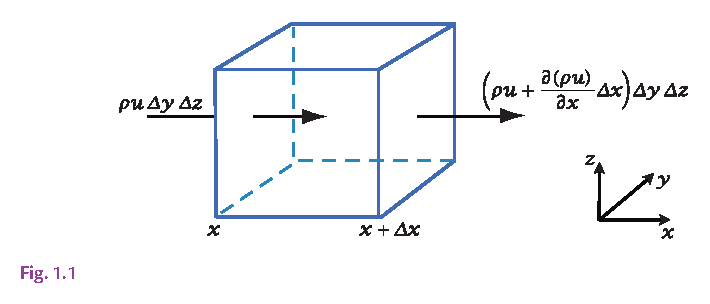
\includegraphics[width=0.8\textwidth]{assets/fig_continuity1.pdf}
  \caption{
    Mass conservation in an rectangular Eulerian control volume.
    The mass convergence, $\partial(\rho u)/\partial x$
    (plus contributions in the $y$ and $z$ directions),
    must be balanced by a density decrease.
    This is Fig. 1.1 in AOFD (Vallis, 2017).
  }
  \label{fig:continuity1}
\end{figure}

\begin{equation}
  \int_V \frac{\partial \rho}{\partial t} dV =
  \rho u + \frac{\partial (\rho u)}{\partial x} \Delta x) \Delta y \Delta z - \rho u \Delta y \Delta z =
\end{equation}

\begin{equation}
  \int_V \frac{\partial \rho}{\partial t} dV =
  \frac{\partial (\rho u)}{\partial x} \Delta x \Delta y \Delta z
\end{equation}
Now, we we allow a flow field to have components in the $y$ and $z$ directions,
the equation becomes:

\begin{equation}
  \int_V \frac{\partial \rho}{\partial t} dV =
  \left[\frac{\partial (\rho u)}{\partial x} + \frac{\partial (\rho v)}{\partial y} + \frac{\partial (\rho w)}{\partial z} \right] \Delta V
\end{equation}
Let $\Delta V \to 0$ to such that any field within $\Delta V$ is uniform to obtain:

\begin{equation}
  \frac{\partial \rho}{\partial t} + \nabla \cdot (\rho \mathbf{u}) = 0
  \label{eq:continuity_eulerian}
\end{equation}
This is the continuity equation in the Eulerian reference frame.

We're not constrained to a rectangular, fixed volume, however.
We can derive this equation for an arbitrary control volume using the divergence
theorem.
The total rate of change of that volume as it moves with the fluid is equal to
the surface integral of the velocity field $\mathbf{u}$ through the surface
$S$ that is bounding the volume $V$ (Fig. \ref{fig:continuity2}).
Mathematically, we can express this as:

\begin{figure}[h]
  \centering
  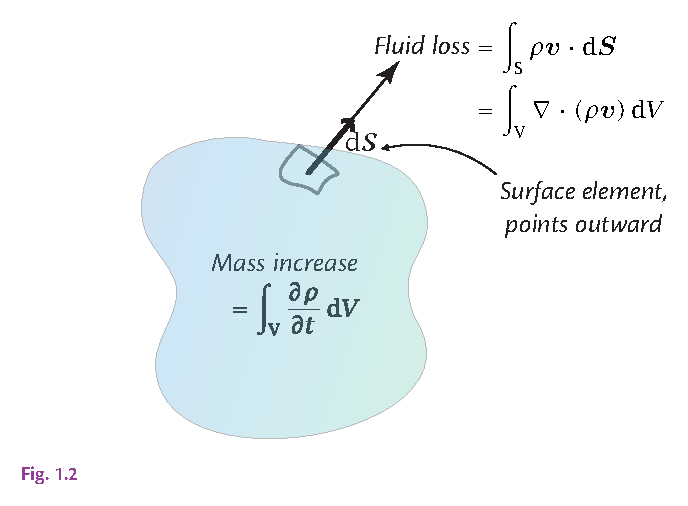
\includegraphics[width=0.7\textwidth]{assets/fig_continuity2.pdf}
  \caption{
    Mass conservation in an arbitrary Eulerian control volume $V$ bounded by a
    surface $S$. The mass increase, $\int_V(\partial \rho/\partial t)dV$
    is equal to the mass flowing into the volume,
    $-\int_S(\rho\mathbf{v}) \cdot d\mathbf{S} = -\int_V \nabla \cdot (\rho\mathbf{v})dV$.
    This is Fig. 1.2 in AOFD (Vallis, 2017).
  }
  \label{fig:continuity2}
\end{figure}

\begin{equation}
  \int_V \frac{\partial \rho}{\partial t} dV = \int_S \rho \mathbf{u} \cdot d\mathbf{S}
\end{equation}
Now, recall the divergence theorem (Eq. \ref{eq:divergence_theorem}) to obtain:

\begin{equation}
  \int_V \frac{\partial \rho}{\partial t} dV = \int_V \nabla \cdot (\rho \mathbf{u}) dV
\end{equation}
Let $\Delta V \to 0$ to integrate and drop $\Delta V$ on both sides to obtain
Eq. \ref{eq:continuity_eulerian}, which is the Eulerian form of the continuity
equation.

\subsubsection{Lagrangian derivation}
\index{Continuity!Lagrangian derivation}

In the Lagrangian frame, we follow a fluid parcel as it moves through space.
Its mass $\rho \Delta V$ is constant by definition, but its density or volume
may change.
Since the mass of the parcel is constant, its Lagrangian derivative is zero:

\begin{equation}
  \frac{d}{dt} (\rho \Delta V) = 0
\end{equation}
Since the mass doesn't change, any change in the density of the parcel must be
balanced by a change in its volume:

\begin{equation}
  \Delta V \frac{d\rho}{dt} + \rho \frac{d\Delta V}{dt} = 0
\end{equation}
Recall that we've already derived the Lagrangian derivative of a volume of the
fluid parcel (Eq. \ref{eq:lagrangian_volume_derivative}), which is the second
term here.
The equation becomes:

\begin{equation}
  \Delta V \frac{d\rho}{dt} + \Delta V \rho \nabla \cdot \mathbf{u} = 0
\end{equation}
Finally, drop $\Delta V$ on both sides to obtain the Lagrangian form of the
continuity equation:

\begin{equation}
  \frac{d\rho}{dt} + \rho \nabla \cdot \mathbf{u} = 0
  \label{eq:continuity_lagrangian}
\end{equation}

Equations \ref{eq:continuity_eulerian} and \ref{eq:continuity_lagrangian} are
two fundamental expressions of the conservation of mass for a fluid.
In one form or another, this equation is a critical component of all weather,
ocean, and climate prediction models.

\subsubsection{Continuity of an incompressible fluid}

Liquids are nearly incompressible, and for them $\frac{d\rho}{dt} = 0$ is a good
approximation.
For an incompressible fluid, the continuity equation simplifies to:

\begin{equation}
  \nabla \cdot \mathbf{u} = 0
  \label{eq:continuity_incompressible}
\end{equation}
Although as simple as it gets, Eq. \ref{eq:continuity_incompressible} is
extremely important in fluid dynamics.

\subsection{Conservation of momentum}
\label{sec:momentum}

Like the conservation of mass, the conservation of momentum is a fundamental
concept in fluid mechanics.
It allows us to predict how the fluid should accelerate due to its state
(i.e. velocity and density) and due to the forces acting on it.
Together, the continuity and momentum conservation
equations form the core of most fluid prediction models, such as weather, ocean,
and climate prediction models.
We will derive the momentum equation in the remainder of this section.
We'll start from the most basic form first and then incrementally introduce
some common forces, such as the pressure gradient force, gravity, and viscosity.

\subsubsection{The first step}

To derive the momentum conservation equation, we will start from the second
Newton's law, which states that the time rate of change of the momentum of a
fluid particle is equal to the net force acting on it.
For a fluid parcel of volume $\Delta V = \int_V dV$ whose momentum per unit mass
is $\rho \mathbf{u}$, the momentum conservation equation is:

\begin{equation}
  \frac{d}{dt} \int_V \rho \mathbf{u} dV = \int_V \mathbf{F} dV
\end{equation}
where $\mathbf{F}$ is the net force per unit volume acting on the fluid parcel.
Let again the volume parcel be very small such that its density and net force
acting on it are uniform. We have:

\begin{equation}
  \rho \frac{d\mathbf{u}}{dt} \Delta V = \mathbf{F} \Delta V
\end{equation}

\begin{equation}
  \rho \frac{d\mathbf{u}}{dt} = \mathbf{F}
\end{equation}
Recall the Lagrangian derivative operator from Eq. \ref{eq:lagrangian_derivative}
to obtain:

\begin{equation}
  \frac{\partial \mathbf{u}}{\partial t} + (\mathbf{u} \cdot \nabla) \mathbf{u} = \frac{\mathbf{F}}{\rho}
  \label{eq:momentum_eulerian}
\end{equation}
This equation states that the acceleration of a fluid parcel at any fixed point
in space is equal to the net force per unit mass acting on it, divided by the
fluid density.
The second term on the left-hand side is the \textit{advection term}\index{Advection}.
It represents the local acceleration of the fluid parcel due to the properties
of the fluid flow itself.
Consider for example a 1-dimensional flow such that the advection term reduces
to $u \frac{\partial u}{\partial x}$.
Notice that the advection term is zero only in two special cases:
when the velocity is zero or when the velocity is spatially uniform.
In all other cases the advection term is non-zero and contributes to the local
acceleration.

Because the advection term is velocity multiplied by its gradient, it is
\textit{nonlinear}\index{Nonlinear}.
This single property of this term makes accurate analysis and prediction of
fluid flows difficult.
For example, the nonlinear advection term is responsible for the existence of
\textit{chaos}\index{Chaos} in fluid flows, where small differences in initial
conditions lead to vastly different outcomes (in popular culture known as the
\textit{butterfly effect}).
One consequence of this in our daily lives is that weather predictability
is limited to a finite lead time horizon, for example one to two weeks depending
on the weather patterns of interest.
If, however, we could assume that either the velocity or its gradient are so
small that they could be neglected, the equation simplifies significantly
and often allows for analytical solutions.

Back to our equation now.
For a 3-dimensional Cartesian flow where the velocity field is $\mathbf{u} = (u, v, w)$
and net forces are $\mathbf{F} = (F_x, F_y, F_z)$, Eq. \ref{eq:momentum_eulerian}
becomes a system of three equations, one for each component of the velocity field.
Recall from the Lagrangian derivative operator that $(\mathbf{u} \cdot \nabla) \mathbf{u}$
is an operator acting on $\mathbf{u}$ (as opposed to divergence of a gradient).
The $(\mathbf{u} \cdot \nabla)$ operator then expands to
$u\frac{\partial}{\partial x} + v\frac{\partial}{\partial y} + w\frac{\partial}{\partial z}$.
Our vector equations becomes a system of three scalar equations:

\begin{equation}
  \frac{\partial u}{\partial t} + u \frac{\partial u}{\partial x} + v \frac{\partial u}{\partial y} + w \frac{\partial u}{\partial z} = \frac{F_x}{\rho}
\end{equation}

\begin{equation}
  \frac{\partial v}{\partial t} + u \frac{\partial v}{\partial x} + v \frac{\partial v}{\partial y} + w \frac{\partial v}{\partial z} = \frac{F_y}{\rho}
\end{equation}

\begin{equation}
  \frac{\partial w}{\partial t} + u \frac{\partial w}{\partial x} + v \frac{\partial w}{\partial y} + w \frac{\partial w}{\partial z} = \frac{F_z}{\rho}
\end{equation}
Each of the prognostic equations for the velocity components thus has exactly
three advective components that correspond to the gradients of the velocity
in each respective direction.

\subsubsection{Incorporating the forces}

Now we should consider what forces may be acting on the fluid.
We distinguish between two types of forces: surface forces and body forces.
Surface forces act on the surface of the fluid parcel due to the motion of the
fluid molecules, in all directions at that surface.
For example, organized motion of molecules into the surface may cause pressure
on that surface, and the sheared motion of molecules (e.g. if flow is
antiparallel to the surface) may cause shear stress on the surface, leading to
the deformation of the fluid parcel.
In contrast, body forces act remotely (meaning, from a distance) on the entire
volume of the fluid parcel because that parcel is immersed in one or more force fields.
Gravity is one such body force, and it's the only one we'll consider here.
Although in Eq. \ref{eq:momentum_eulerian} we wrote the net force as $\mathbf{F}$,
it's useful to write it as the sum of body forces $\mathbf{F}_b$ and surface
forces $\mathbf{F}_s$:

\begin{equation}
  \frac{\partial \mathbf{u}}{\partial t} + (\mathbf{u} \cdot \nabla) \mathbf{u} = \frac{1}{\rho} (\mathbf{F}_s + \mathbf{F}_b)
\end{equation}

Let's derive the surface forces first.
We want to find out the local change of momentum only due to the surface forces.
Analogous to how the flow through the volume determined the rate of change of
density inside that volume, as we saw in the continuity equation
(Eq. \ref{eq:continuity_eulerian}), the change in momentum inside the volume
is determined by the surface forces acting on the volume (Fig. \ref{fig:momentum1}).

\begin{figure}[h]
  \centering
  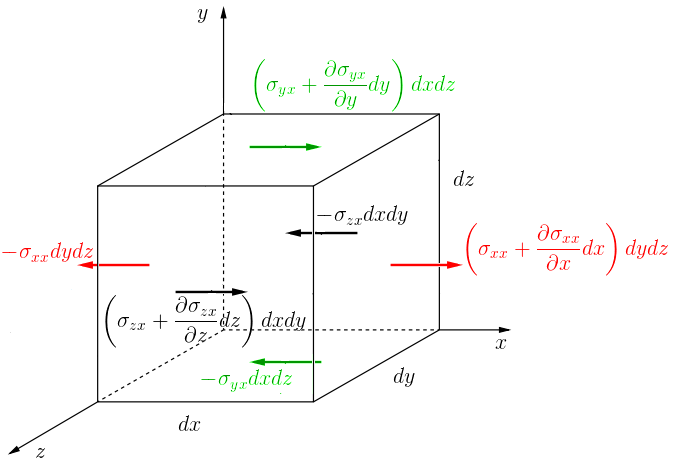
\includegraphics[width=0.8\textwidth]{assets/fig_momentum1.png}
  \caption{
    Normal components of the stress tensor $\mathbf{\sigma}$ acting on a fluid parcel.
    Reproduced from \url{https://en.wikipedia.org/wiki/Cauchy_momentum_equation}
    under the CC BY-SA 4.0 license.
  }
  \label{fig:momentum1}
\end{figure}

Mathematically, we can express this change as:

\begin{equation}
  \int_V \mathbf{F_s} dV = \int_S \boldsymbol{\sigma} \cdot d\mathbf{S}
\end{equation}
where $\boldsymbol{\sigma}$ is the second-order stress tensor acting on the
surface $S$ of the fluid parcel.
As before, recall the divergence theorem (Eq. \ref{eq:divergence_theorem}) to obtain:

\begin{equation}
  \int_V \mathbf{F_s} dV = \int_V \nabla \cdot \boldsymbol{\sigma} dV
\end{equation}

\begin{equation}
  \mathbf{F_s} = \nabla \cdot \boldsymbol{\sigma}
\end{equation}
The surface force thus equals the divergence of the stress tensor.
Insert this into Eq. \ref{eq:momentum_eulerian} to get our new form of
the momentum equation:

\begin{equation}
  \frac{\partial \mathbf{u}}{\partial t} + (\mathbf{u} \cdot \nabla) \mathbf{u} =
  \frac{1}{\rho} \nabla \cdot \boldsymbol{\sigma} + \frac{\mathbf{F}_b}{\rho}
  \label{eq:momentum_cauchy}
\end{equation}
This form of the momentum equation is often called the
\textit{Cauchy momentum equation}\index{Momentum equation!Cauchy}.

Let's now look at what this stress tensor divergence term
$\nabla \cdot \boldsymbol{\sigma}$ is.

\subsubsection{Pressure gradient}

There is a fundamental difference in the meaning of the diagonal and off-diagonal
components of the stress tensor.
The diagonal components of the stress tensor, $\sigma_{xx}$, $\sigma_{yy}$, and
$\sigma_{zz}$, represent the normal stress components, i.e. the force per unit
area acting on a surface element that is oriented in the $x$, $y$, and $z$
directions, respectively.
The off-diagonal components of the stress tensor represent the shear stress
components, each acting on all three surfaces.
For example, $\sigma_{xy}$ represents the $x$-component of the stress tensor
acting on the surface that is perpendicular to the $y$-axis.
Let's write out the stress tensor in Cartesian coordinates:

\begin{equation}
  \boldsymbol{\sigma} = \begin{bmatrix}
    \sigma_{xx} & \sigma_{xy} & \sigma_{xz} \\
    \sigma_{yx} & \sigma_{yy} & \sigma_{yz} \\
    \sigma_{zx} & \sigma_{zy} & \sigma_{zz}
  \end{bmatrix}
\end{equation}

This tensor can be decomposed into its normal and shear components:

\begin{equation}
  \boldsymbol{\sigma} = -p \mathbf{I} + \boldsymbol{\tau}
  \label{eq:stress_tensor_decomposition}
\end{equation}
where $p$ is the pressure, $\mathbf{I}$ is the identity tensor\index{Tensor!Identity},
and $\boldsymbol{\tau}$ is the deviatoric stress tensor, or, the viscous shear
stress tensor\index{Stress!Shear}.
Written out explicitly in Cartesian coordinates and using Eq.
\ref{eq:stress_tensor_decomposition}, the stress tensor is:

\begin{equation}
  \boldsymbol{\sigma} = \begin{bmatrix}
    -p + \tau_{xx} & \tau_{xy} & \tau_{xz} \\
    \tau_{yx} & -p + \tau_{yy} & \tau_{yz} \\
    \tau_{zx} & \tau_{zy} & -p + \tau_{zz}
  \end{bmatrix}
\end{equation}

The divergence of the stress tensor is then:

\begin{equation}
  \nabla \cdot \boldsymbol{\sigma} = - \nabla p + \nabla \cdot \boldsymbol{\tau}
\end{equation}
Let's insert this into Eq. \ref{eq:momentum_eulerian} to get our new form of
the momentum equation:

\begin{equation}
  \frac{\partial \mathbf{u}}{\partial t} + (\mathbf{u} \cdot \nabla) \mathbf{u} =
  - \frac{1}{\rho} \nabla p + \frac{1}{\rho} \nabla \cdot \boldsymbol{\tau} + \frac{\mathbf{F}_b}{\rho}
  \label{eq:momentum_cauchy_with_shear}
\end{equation}

Pressure is one of the fluid properties that determine its state.
Collective, organized, motion of molecules at a macroscopic scale induces
pressure on a surface and an associated force acting normal to that surface.
Recall that the surface vector is normal to the surface and pointing outward,
and the force acting on the fluid surface is oriented inward, thus the minus sign.

In an ideal, \textit{inviscid} fluid, that is, a fluid that exhibits no viscous
forces, the stress tensor $\boldsymbol{\sigma}$ is only composed of the diagonal
terms (pressure), and the divergence of the stress tensor is zero.
Dropping $\nabla \cdot \boldsymbol{\tau}$ and the body forces $\mathbf{F}_b$ for
now, the Cauchy momentum equation simplifies to:

\begin{equation}
  \frac{\partial \mathbf{u}}{\partial t} + (\mathbf{u} \cdot \nabla) \mathbf{u} =
  - \frac{1}{\rho} \nabla p
  \label{eq:momentum_euler}
\end{equation}
This form of the momentum equation is often called the \textit{Euler equation}.
\index{Momentum equation!Euler}

\subsubsection{Viscous forces}
\label{sec:viscous_forces}

Now, let's look at the shear stress tensor divergence $\nabla \cdot \boldsymbol{\tau}$.
Written out explicitly as a matrix of all its components, $\boldsymbol{\tau}$ is:

\begin{equation}
  \boldsymbol{\tau} = \begin{bmatrix}
    \tau_{xx} & \tau_{xy} & \tau_{xz} \\
    \tau_{yx} & \tau_{yy} & \tau_{yz} \\
    \tau_{zx} & \tau_{zy} & \tau_{zz}
  \end{bmatrix}
\end{equation}
The diagonal components of the deviatoric stress tensor are the normal stresses,
while the off-diagonal components are the shear stresses.
The normal stresses are non-zero only in compressible fluids ($\nabla \cdot \mathbf{u} \neq 0$),
while the shear stresses are zero in non-viscous flows.
The divergence of this tensor, written out explicitly as a matrix of all its
components, is:

\begin{equation}
  \nabla \cdot \boldsymbol{\tau} = \begin{bmatrix}
    \frac{\partial \tau_{xx}}{\partial x} + \frac{\partial \tau_{yx}}{\partial y} + \frac{\partial \tau_{zx}}{\partial z} \\
    \frac{\partial \tau_{xy}}{\partial x} + \frac{\partial \tau_{yy}}{\partial y} + \frac{\partial \tau_{zy}}{\partial z} \\
    \frac{\partial \tau_{xz}}{\partial x} + \frac{\partial \tau_{yz}}{\partial y} + \frac{\partial \tau_{zz}}{\partial z}
  \end{bmatrix}
\end{equation}

Now, write out \ref{eq:momentum_cauchy_with_shear} as a system of three scalar
equations, one for each component of the velocity field, and insert the shear
stress divergence terms to get:

\begin{equation}
  \frac{\partial u}{\partial t} + 
  u \frac{\partial u}{\partial x} + 
  v \frac{\partial u}{\partial y} + 
  w \frac{\partial u}{\partial z} = 
  - \frac{1}{\rho} \frac{\partial p}{\partial x} + 
  \frac{1}{\rho} \left( \frac{\partial \tau_{xx}}{\partial x} + \frac{\partial \tau_{yx}}{\partial y} + \frac{\partial \tau_{zx}}{\partial z} \right) + 
  \frac{F_x}{\rho}
\end{equation}

\begin{equation}
  \frac{\partial v}{\partial t} + 
  u \frac{\partial v}{\partial x} + 
  v \frac{\partial v}{\partial y} + 
  w \frac{\partial v}{\partial z} = 
  - \frac{1}{\rho} \frac{\partial p}{\partial y} + 
  \frac{1}{\rho} \left( \frac{\partial \tau_{xy}}{\partial x} + \frac{\partial \tau_{yy}}{\partial y} + \frac{\partial \tau_{zy}}{\partial z} \right) + 
  \frac{F_y}{\rho}
\end{equation}

\begin{equation}
  \frac{\partial w}{\partial t} + 
  u \frac{\partial w}{\partial x} + 
  v \frac{\partial w}{\partial y} + 
  w \frac{\partial w}{\partial z} = 
  - \frac{1}{\rho} \frac{\partial p}{\partial z} + 
  \frac{1}{\rho} \left( \frac{\partial \tau_{xz}}{\partial x} + \frac{\partial \tau_{yz}}{\partial y} + \frac{\partial \tau_{zz}}{\partial z} \right) + 
  \frac{F_z}{\rho}
\end{equation}
Each of the prognostic equations for the velocity components thus has exactly
one pressure gradient and two shear stress gradient terms, all arising from the
surface forces.

Experimentally, it was found that the viscous shear stress tensor $\boldsymbol{\tau}$
is proportional to the gradient of the velocity field, i.e. $\boldsymbol{\tau} = \mu \nabla \mathbf{u}$.
This property of the fluid makes it a so-called \textit{Newtonian fluid}\index{Fluid!Newtonian}.
The proportionality constant $\mu$ is the dynamic viscosity and depends on the
fluid properties and temperature.
Inserting this into Eq. \ref{eq:momentum_cauchy_with_shear} and assuming
incompressibility, we get:

\begin{equation}
  \frac{\partial \mathbf{u}}{\partial t} + (\mathbf{u} \cdot \nabla) \mathbf{u} =
  - \frac{1}{\rho} \nabla p + \frac{1}{\rho} \nabla \cdot (\mu \nabla \mathbf{u}) +
  \frac{\mathbf{F}_b}{\rho}
\end{equation}
We can further simplify this equation by assuming that the viscosity is constant
and that the flow is incompressible.
This allows us to neglect the viscous stress gradient term, leading to the
\textit{Navier-Stokes equation}\index{Momentum equation!Navier-Stokes}.

\begin{equation}
  \frac{\partial \mathbf{u}}{\partial t} + (\mathbf{u} \cdot \nabla) \mathbf{u} =
  - \frac{1}{\rho} \nabla p + \nu \nabla^2 \mathbf{u} +
  \frac{\mathbf{F}_b}{\rho}
  \label{eq:momentum_navier_stokes}
\end{equation}
where $\nu = \frac{\mu}{\rho}$ is the kinematic viscosity.
The $\nabla^2$ operator is often called the \textit{Laplacian}\index{Laplacian}.
It is a second-order differential operator that appears in many partial
differential equations, including the heat equation, the wave equation, and
the Laplace equation.
More on these later.

Let's now look at the body forces to conclude our derivation.

\subsubsection{Gravity}

As we mentioned earlier, gravity is the only body force we'll consider here.
The force of gravity per unit mass is given by $\mathbf{g} = (0, 0, -g)$,
where $g$ is the gravitational acceleration.
Here we're assuming that the gravitational acceleration is constant and always
points downward.
Insert this into Eq. \ref{eq:momentum_navier_stokes} and assuming
incompressibility, we get:

\begin{equation}
  \frac{\partial \mathbf{u}}{\partial t} + (\mathbf{u} \cdot \nabla) \mathbf{u} =
  - \frac{1}{\rho} \nabla p + \mathbf{g} + \nu \nabla^2 \mathbf{u}
\end{equation}

Written out explicitly, we get:

\begin{equation}
  \frac{\partial u}{\partial t} + 
  u \frac{\partial u}{\partial x} + 
  v \frac{\partial u}{\partial y} + 
  w \frac{\partial u}{\partial z} = 
  - \frac{1}{\rho} \frac{\partial p}{\partial x} + \nu \left( \frac{\partial^2 u}{\partial x^2} + \frac{\partial^2 u}{\partial y^2} + \frac{\partial^2 u}{\partial z^2} \right)
\end{equation}

\begin{equation}
  \frac{\partial v}{\partial t} + 
  u \frac{\partial v}{\partial x} + 
  v \frac{\partial v}{\partial y} + 
  w \frac{\partial v}{\partial z} = 
  - \frac{1}{\rho} \frac{\partial p}{\partial y} + \nu \left( \frac{\partial^2 v}{\partial x^2} + \frac{\partial^2 v}{\partial y^2} + \frac{\partial^2 v}{\partial z^2} \right)
\end{equation}

\begin{equation}
  \frac{\partial w}{\partial t} + 
  u \frac{\partial w}{\partial x} + 
  v \frac{\partial w}{\partial y} + 
  w \frac{\partial w}{\partial z} = 
  - \frac{1}{\rho} \frac{\partial p}{\partial z} - g + \nu \left( \frac{\partial^2 w}{\partial x^2} + \frac{\partial^2 w}{\partial y^2} + \frac{\partial^2 w}{\partial z^2} \right)
  \label{eq:momentum_navier_stokes_scalar_w}
\end{equation}
This completes the full system of momentum conservation equations in the
Cartesian coordinate system.

\subsection{Hydrostatic balance}

Take Eq. \ref{eq:momentum_navier_stokes_scalar_w} and assume that the vertical
acceleration $\frac{dw}{dt}$ is small compared to $g$, and that the spatial
variations of $w$ are small.
We can then drop the $\frac{dw}{dt}$ and $\nu \nabla^2 w$ terms to get the
\textit{hydrostatic approximation}\index{Hydrostatic approximation}:

\begin{equation}
  \frac{\partial p}{\partial z} = - \rho g
  \label{eq:hydrostatic_approximation}
\end{equation}
which states that the vertical pressure gradient is governed by the density
of the fluid and the gravitational acceleration.
It's often a good approximation for large-scale atmospheric and oceanic flows,
where the vertical variations of the horizontal velocity components are much
smaller than the horizontal variations of the vertical velocity component.
Notice however that the hydrostatic approximation does not imply that there
is no vertical motion or that it does not vary over time.
Instead, according to the continuity equation (Eq. \ref{eq:continuity_lagrangian}),
it means that the vertical motion is completely governed by the change in
density and the divergence of the horizontal velocity field.
Further, if the flow is incompressible ($\nabla \cdot \mathbf{u} = 0$),
we get:

\begin{equation}
  \frac{\partial w}{\partial z} = - \frac{\partial u}{\partial x} - \frac{\partial v}{\partial y}
  \label{eq:hydrostatic_continuity}
\end{equation}
This relationship will prove to be extremely useful in ocean applications where
only the horizontal velocity field is resolved.
For example, a group of ocean surface drifters converging towards a region is
indicative of downwelling (downward motion in the ocean) in that region.
Another example is that of ocean circulation models, which are typically
designed as hydrostatic.
In the case of such models, the horizontal components of the velocity are
prognostic variables, and the vertical velocity is diagnosed using
Eq. \ref{eq:hydrostatic_continuity}.

\subsection{Equation of state}

Now that we have derived the mass and momentum conservation equations, let's
write them out together in vector form:

\begin{equation}
  \frac{\partial \mathbf{u}}{\partial t} + (\mathbf{u} \cdot \nabla) \mathbf{u} =
  - \frac{1}{\rho} \nabla p + \mathbf{g} + \nu \nabla^2 \mathbf{u}
  \label{eq:momentum_navier_stokes_state}
\end{equation}

\begin{equation}
  \frac{\partial \rho}{\partial t} + \nabla \cdot (\rho \mathbf{u}) = 0
  \label{eq:continuity_eulerian_state}
\end{equation}
Momentum and mass conservation equations are prognostic equations for the
vector velocity field $\mathbf{u}$ and the scalar density field $\rho$,
respectively.
Notice the one remaining unknown: the scalar pressure field $p$.
As of now, we have a system of two independent equations for the three unknowns:
$\mathbf{u}$, $p$, and $\rho$.
We need one more equation to close the system---the
\textit{equation of state}\index{Equation of state}---to relate the pressure to
the other properties of the fluid, such as temperature, density, and
composition.

The prognostic equations that we have derived so far describe equally well
the evolution of both the atmosphere and the ocean, despite their significant
differences.
The equation of state is where our systems of governing equations for the ocean
and the atmosphere begin to diverge.
Namely, the atmosphere is a mixture of dry air and water vapor, and the
ocean is composed of liquid water with varying amounts of dissolved salts.
These differences will reflect in the choice of the equation of state to use
in each of these systems.

\subsubsection{In the atmosphere}

In the atmospheres, \textit{ideal gas law}\index{Equation of state!Ideal gas law}
is often used as the equation of state:

\begin{equation}
  p = \rho R T
  \label{eq:ideal_gas_law}
\end{equation}
where $R$ is the specific gas constant for the gas in question, and $T$ is the
temperature.
For the moist air, we need account for both the properties of dry air
($R_d \approx 287 J kg^{-1} K^{-1}$) and those of water vapor
($R_v \approx 461 J kg^{-1} K^{-1}$).
The equation of state for moist air relies on the so-called
\textit{virtual temperature}\index{Virtual temperature} to account for the
moisture in the air:

\begin{equation}
  p = \rho R_d T_v
\end{equation}
where:

\begin{equation}
  T_v = T \left[1 + q \left(\frac{R_v}{R_d} - 1 \right) \right]
\end{equation}
where $q$ is the specific humidity of the air.
So, the equation of state for moist air is:

\begin{equation}
  p = \rho R_d T \left[1 + q \left(\frac{R_v}{R_d} - 1 \right) \right]
  \label{eq:equation_of_state_atmosphere}
\end{equation}

Recall that we intended to close our system of equations by finding the
equation for pressure.
Although we did solve for pressure, it seems that we introduced two new
unknown variables: the temperature $T$ and the specific humidity $q$.
Each of these variables are governed by their own conservation equations,
akin to that for density, but with the addition of source and sink terms
that control their production and loss:

\begin{equation}
  \frac{\partial T}{\partial t} + (\mathbf{u} \cdot \nabla) T = \dot{S}_T
  \label{eq:temperature_equation}
\end{equation}

\begin{equation}
  \frac{\partial q}{\partial t} + (\mathbf{u} \cdot \nabla) q = \dot{S}_q
  \label{eq:specific_humidity_equation}
\end{equation}
where $\dot{S}_T$ and $\dot{S}_q$ are the sources and sinks of temperature and
specific humidity, respectively.

Although we won't delve further into the details behind the sources and sinks
of temperature and specific humidity in the atmosphere, we can denote these
equations as completing the full system of prognostic equations for the
atmosphere: Eqs. \ref{eq:momentum_navier_stokes_state}, 
\ref{eq:continuity_eulerian_state},
\ref{eq:equation_of_state_atmosphere},
\ref{eq:temperature_equation}, and
\ref{eq:specific_humidity_equation}.
These equations form the basis of many weather and climate prediction models.

\subsubsection{In the ocean}

Ideal gas law (Eq. \ref{eq:ideal_gas_law}) doesn't apply to liquids and the
equation of state for seawater is not easily derived.
Instead, we assume that the ocean is a single-component fluid, and we use the
density field $\rho$ as the equation of state.

\begin{equation}
  \rho = \rho(T, S, p) \\
  = \rho_0 \left[ 1 - \beta_T(T-T_0) + \beta_S(S-S_0) + \beta_p(p-p_0) \right]
  \label{eq:equation_of_state_ocean}
\end{equation}
where $\rho_0$ is the reference density at the reference temperature $T_0$,
salinity $S_0$, and pressure $p_0$.
The coefficients $\beta_T$, $\beta_S$, and $\beta_p$ are the thermal expansion
coefficient, the saline contraction coefficient, and the pressure
coefficient, respectively.
This form of the equation of state is a linear equation of state (as in, the
dependence of density on temperature, salinity, and pressure each is linear).
Dependence of density on temperature and salinity at two different pressure
levels is shown in Fig. \ref{fig:seawater_eqstate}.
Higher order equations of state are often used for higher accuracy, however
they're out of scope for this course.

\begin{figure}[h]
  \centering
  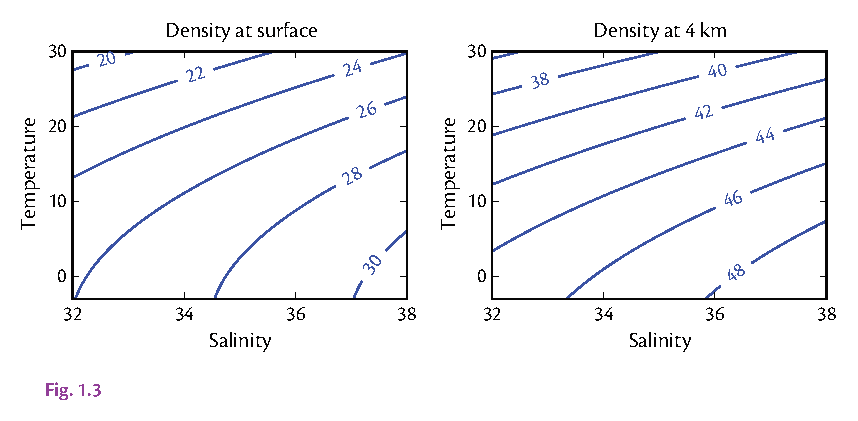
\includegraphics[width=\textwidth]{assets/fig_seawater_eqstate.pdf}
  \caption{
    Contours of density as a function of temperature and salinity for seawater.
    Contour labels are (density - 1000) kg m$^{-3}$.
    Left panel: at sea-level ($p = 10^5\ Pa$, or 1000 mb).
    Right panel: at $p = 4 \times 10^7\ Pa$ (about 4 km depth).
    In both cases the contours are slightly convex, so that if two parcels at
    the same density but different temperatures and salinities are mixed, the
    resulting parcel is of higher density.
    (The average temperature is not exactly conserved on mixing, but it very
    nearly is.)
    This is Fig. 1.3 in AOFD (Vallis, 2017).
  }
  \label{fig:seawater_eqstate}
\end{figure}

Like we did in the case of atmosphere, here we need to additional prognostic
equations, one of temperature and another for salinity:

\begin{equation}
  \frac{\partial T}{\partial t} + (\mathbf{u} \cdot \nabla) T = \dot{S}_T
  \label{eq:temperature_equation_ocean}
\end{equation}

\begin{equation}
  \frac{\partial S}{\partial t} + (\mathbf{u} \cdot \nabla) S = \dot{S}_S
  \label{eq:salinity_equation_ocean}
\end{equation}
where $\dot{S}_T$ and $\dot{S}_S$ are the sources and sinks of water temperature
and salinity, respectively.

Equations \ref{eq:momentum_navier_stokes_state},
\ref{eq:continuity_eulerian_state},
\ref{eq:equation_of_state_ocean},
\ref{eq:temperature_equation_ocean}, and
\ref{eq:salinity_equation_ocean} are the governing equations used in most
numerical ocean circulation models.

\subsection{Nondimensionalization and scaling}
\label{sec:nondimensionalization_and_scaling}

A useful technique to simplify the analysis of the governing equations is to
scale the variables using characteristic values for each of the variables.
This is known as \textit{nondimensionalization}\index{Nondimensionalization}
or \textit{scaling the equations}\index{Scaling}.
In practice, for each (dependent or independent) variable $x$ in the equations,
we define a characteristic value $X$.
For example, for the velocity $\mathbf{u}$, we may pick the characteristic
value of $U = 1\ m\ s^{-1}$ or $U = 10\ m\ s^{-1}$ for the ocean or atmosphere,
respectively.
We then divide each term in the equations by the characteristic value to
obtain a nondimensional (unitless) number.
This helps us identify the important parameters that govern the behavior of
the system and to group terms in the equations that are of similar magnitudes.
This is especially useful for large-scale flows, where the length and time
scales can vary over several orders of magnitude.

For example, let's look at the vector equation for horizontal momentum
(thus, ignoring $\mathbf{g}$ for now):

\begin{equation}
  \frac{\partial \mathbf{u}}{\partial t} + (\mathbf{u} \cdot \nabla) \mathbf{u} =
  - \frac{1}{\rho} \nabla p + \nu \nabla^2 \mathbf{u}
\end{equation}

The characteristic scales for each term are:

\begin{equation}
  \frac{\partial \mathbf{u}}{\partial t} \sim \frac{U}{T}
\end{equation}

\begin{equation}
  (\mathbf{u} \cdot \nabla) \mathbf{u} \sim \frac{U^2}{L}
\end{equation}

\begin{equation}
  - \frac{1}{\rho} \nabla p \sim \frac{1}{\rho} \frac{P}{L}
\end{equation}

\begin{equation}
  \nu \nabla^2 \mathbf{u} \sim \nu \frac{U}{L^2}
\end{equation}
where $U$, $T$, $L$, and $P$ are the characteristic scales for the velocity,
time, length, and pressure, respectively.
So, if for a given flow we can estimate these characteristic values, we can
easily determine which terms are important and which can be neglected.
This is the basis of scaling arguments in fluid mechanics.

This approach also enables characterizing the flows in terms of
nondimensional numbers.
For example, to describe how turbulent or laminar a flow is, it's useful to
relate the inertial to the viscous terms in the momentum equation.
Their ratio is called the  \textit{Reynolds number}\index{Reynolds number}:

\begin{equation}
  \frac{(\mathbf{u} \cdot \nabla) \mathbf{u}}{\nu \nabla^2 \mathbf{u}} \sim
  \frac{\frac{U^2}{L}}{\frac{\nu U}{L^2}} = \frac{UL}{\nu} \equiv \text{Re}
  \label{eq:reynolds_number}
\end{equation}
You see that the Reynolds number is proportional to the velocity and length
scales each, and inversely proportional to the viscosity.
A larger Reynolds number corresponds to a more turbulent flow.

\subsection{Exercises}

\begin{enumerate}
  \item Derive the Lagrangian form of the continuity equation from
  the Eulerian form and vice versa. What is the key equation that relates the
  two forms?

  \item Write out the Cauchy, Euler, and Navier-Stokes equations in vector form
  and discuss their similarities and differences.
  Give examples of flows that are well described by each of these equations.

  \item Write a computer program that calculates the divergence of a second-order
  tensor in a Cartesian, 3-dimensional coordinate system.

  \item Consider two opposing, horizontal, surface currents along the $x$-axis.
  In the vertical they uniformly span a mixed layer that extends from the
  surface to the depth of 20 meters, with a magnitude of 1 m s$^{-1}$.
  The two currents meet at a stagnation zone that is 100 meters wide.
  Calculate the downwelling velocity at the bottom of the mixed layer.
  Assume $\nabla \cdot \mathbf{u} = 0$, no change in mean sea level, and no
  flow in the $y$-direction.

  \item Write a function in your favorite programming language that takes a
  value of temperature, salinity, and pressure and returns the density of
  seawater. Assume linear dependence of density on temperature, salinity, and
  pressure. Take the thermal expansion coefficient to be $\beta_T = 1.67 \times 10^{-4} K^{-1}$,
  the Haline contraction coefficient to be $\beta_S = 7.8 \times 10^{-4} g\ kg^{-1}$,
  and the compressibility coefficient to be $\beta_p = 4.4 \times 10^{-10} Pa^{-1}$.
  Take the reference density to be $\rho_0 = 1027\ kg\ m^{-3}$, the reference
  temperature to be $T_0 = 283\ K$, the reference salinity to be $S_0 = 35 g\ kg^{-1}$,
  and the reference pressure to be $p_0 = 10^5\ Pa$.
  When you implement your function, calculate the density of seawater for the
  range of temperatures from -2 to 30 degrees Celsius, and salinities from 20 to
  40 g/kg, and plot it as a contour plot as a function of temperature and salinity.
  Make such plots for pressure values of $10^5$, $10^6$, and $10^7$ Pa.

  \item Calculate the Reynolds number for:
  (a) a synoptic-scale mid-latitude cyclone in the atmosphere;
  (b) an mesoscale ocean eddy;
  (c) a river inflow into the ocean;
  (d) a breaking ocean surface wave;
  (e) water flowing through a pipe with a diameter of 0.1 m and flow speed of 1 m s$^{-1}$.
  Assume $\nu = 10^{-5} m^2 s^{-1}$ for air and $\nu = 10^{-6} m^2 s^{-1}$ for water.

\end{enumerate}

\subsection*{Further reading}

\begin{itemize}
  \item Sections 1.2-1.4 of \textit{EAOD} by Vallis
  \item Sections 4.1-4.6 of \textit{Fluid Mechanics} by Kundu, Cohen, and Dowling
\end{itemize}

\newpage
\section{Rotating flows}

Fluids behave somewhat differently when in a rotating reference frame, for
example on the surface of a rotating planet.
In this chapter we explore the effects of rotation on the flow.
We begin by deriving the temporal derivative of a general vector in a rotating
reference frame, and then apply it to find the velocity and acceleration in such
a frame.
From there we derive the centrifugal and Coriolis forces, and discuss their
implications for geophysical flows.

\subsection{Rate of change of a rotating vector}

Before determining the what the velocity and acceleration should appear like
in a rotating reference frame (i.e. on the surface of a rotating planet), we
first need to understand how a vector that is fixed in the rotating frame
appears to change over time to the observer in the inertial (fixed) frame.
To do that, consider a vector $\mathbf{C}$ that rotates around an axis at a
constant angular velocity $\mathbf{\Omega}$ (Fig. \ref{fig:rotating_vector}).
The angular velocity $\mathbf{\Omega}$ is the rate of change of the angle in
the plane that is perpendicular to the axis of rotation, and is thus
$\frac{d\lambda}{dt}$.
A unit vector $\mathbf{m}$ is oriented in the direction of the rate of change
of $\mathbf{C}$, and is perpendicular to both $\mathbf{C}$ and $\mathbf{\Omega}$.
We will assume that $\mathbf{\Omega}$ is constant.
This is a generally good assumption for the rotation rates of planets, at least
on time scales that we are interested in.
A small change in $\mathbf{C}$ can then be expressed as:

\begin{figure}[h]
  \centering
  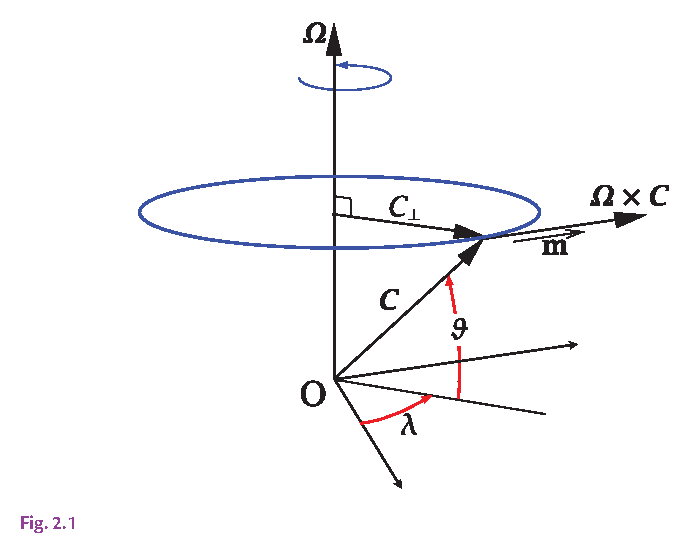
\includegraphics[width=0.8\textwidth]{assets/fig_rotating_vector.pdf}
  \caption{
    A vector $\mathbf{C}$ rotating at an angular velocity $\mathbf{\Omega}$.
    It appears to be a constant vector in the rotating frame, whereas in the
    inertial frame it rotates according to
    $\left(d\mathbf{C}/dt\right)_I = \mathbf{\Omega} \times \mathbf{C}$.
    This is Fig. 2.1 in AOFD (Vallis, 2017).
  }
  \label{fig:rotating_vector}
\end{figure}

\begin{equation}
  \delta \mathbf{C} = |\mathbf{C}| \cos\theta\ \delta \lambda\ \mathbf{m}
\end{equation}
The change in $\mathbf{C}$ is thus proportional to:
its magnitude;
the cosine of the angle between $\mathbf{C}$ and the horizontal plane
(\textit{i.e.} the plane perpendicular to $\mathbf{\Omega}$);
the change in $\lambda$;
and, the unit vector $\mathbf{m}$.
Notice now that using the definition of the cross product (Eq. \ref{eq:cross_product_magnitude}),
we can write the change in $\mathbf{C}$ as:

\begin{equation}
  \delta \mathbf{C} = |\mathbf{C}| |\mathbf{\Omega}| \sin(\pi/2 - \theta)\ \mathbf{m}\ \delta t =
  \mathbf{\Omega} \times \mathbf{C}\ \delta t
\end{equation}
so the rate of change of a rotating vector, when observed from a fixed, inertial
frame is the cross product of the angular velocity and the vector itself:

\begin{equation}
  \left(\frac{d\mathbf{C}}{dt}\right)_I = \mathbf{\Omega} \times \mathbf{C}
\end{equation}
Going forward, we will use the subscript $I$ to denote the inertial frame,
non-rotating reference frame.

Imagine now that you're standing on top of the rotating vector $\mathbf{C}$,
and are still relative to that rotating reference frame, much like standing
still on the surface of a rotating planet.
To you as the observer in the rotating frame, the vector $\mathbf{C}$ appears
to not change in any way.
Consider now another vector $\mathbf{B}$ that may change (in direction or
magnitude, or both) in the rotating reference frame.
We can then say that the rate of change of $\mathbf{B}$ in the inertial frame
is the vector sum of its two rates of change:
The rate of change of $\mathbf{B}$ in the rotating frame, and the rate of
change of the rotating frame itself:

\begin{equation}
  \left(\frac{d\mathbf{B}}{dt}\right)_I = \left(\frac{d\mathbf{B}}{dt}\right)_R + \mathbf{\Omega} \times \mathbf{B}
  \label{eq:rate_of_change_rotating_vector}
\end{equation}

We now have a useful tool to use to determine the velocity and acceleration in
a rotating frame, such as that of of the surface of a rotating planet.

\subsection{Velocity and acceleration in a rotating frame}

Consider now a position vector $\mathbf{r}$ that locates a parcel in the rotating
frame.
The velocity of the parcel in the inertial frame is then given by the rate of
change of the position vector.
Apply Eq. \ref{eq:rate_of_change_rotating_vector} to $\mathbf{r}$ to get:

\begin{equation}
  \left( \frac{d\mathbf{r}}{dt} \right)_I = \left( \frac{d\mathbf{r}}{dt} \right)_R + \mathbf{\Omega} \times \mathbf{r}
\end{equation}
As the time derivative of a position vector is velocity by definition, we can
write this as:

\begin{equation}
  \mathbf{u}_I = \mathbf{u}_R + \mathbf{\Omega} \times \mathbf{r}
  \label{eq:inertial_velocity}
\end{equation}
This relates the inertial and rotating velocities.
Recall that we are interested in accelerations, as it's the acceleration that
we solve for in the Navier-Stokes equations and relate to the forces that act
on the fluid.
We know that the acceleration is the rate of change of velocity, so let's apply
Eq. \ref{eq:rate_of_change_rotating_vector} to the rotating velocity:

\begin{equation}
  \left( \frac{d\mathbf{u}_R}{dt} \right)_I = \left( \frac{d\mathbf{u}_R}{dt} \right)_R + \mathbf{\Omega} \times \mathbf{u}_R
  \label{eq:inertial_acceleration}
\end{equation}
Now, use Eq. \ref{eq:inertial_velocity} to substitute for $\mathbf{u}_I$ in
Eq. \ref{eq:inertial_acceleration}:

\begin{equation}
  \left( \frac{d\left(\mathbf{u}_I - \mathbf{\Omega} \times \mathbf{r}\right)}{dt} \right)_I = 
  \left( \frac{d\mathbf{u}_R}{dt} \right)_R + \mathbf{\Omega} \times \mathbf{u}_R
\end{equation}

\begin{equation}
  \left( \frac{d \mathbf{u}_I}{dt} \right)_I =
  \left( \frac{d \mathbf{u}_R}{dt} \right)_R +
  \mathbf{\Omega} \times \mathbf{u}_R +
  \frac{d\mathbf{\Omega}}{dt} \times \mathbf{r} +
  \mathbf{\Omega} \times \left( \frac{d\mathbf{r}}{dt} \right)_I
  \label{eq:inertial_acceleration_from_rotating}
\end{equation}
Recall that:

\begin{equation}
  \left( \frac{d \mathbf{r}}{dt} \right)_I =
  \left( \frac{d \mathbf{r}}{dt} \right)_R +
  \mathbf{\Omega} \times \mathbf{r} =
  \left( \mathbf{u}_R + \mathbf{\Omega} \times \mathbf{r} \right)
  \label{eq:inertial_velocity_from_rotating}
\end{equation}
If $\mathbf{\Omega}$ is constant, as we have assumed at the beginning,
inserting Eq. \ref{eq:inertial_velocity_from_rotating} into Eq.
\ref{eq:inertial_acceleration_from_rotating} yields:

\begin{equation}
  \left( \frac{d \mathbf{u}_R}{dt} \right)_R =
  \left( \frac{d \mathbf{u}_I}{dt} \right)_I -
  2 \mathbf{\Omega} \times \mathbf{u}_R -
  \mathbf{\Omega} \times \left( \mathbf{\Omega} \times \mathbf{r} \right)
  \label{eq:rotating_acceleration}
\end{equation}

The interpretation of the terms in Eq. \ref{eq:rotating_acceleration} is:

\begin{itemize}
  \item $\left( \frac{d \mathbf{u}_R}{dt} \right)_R$, is the rate of change of
  the relative velocity as observed in the rotating frame.
  This is the rate of change of the velocity that you would measure with an
  anemometer or current meter if position fixed relative to the rotating planet's
  surface. 

  \item $\left( \frac{d \mathbf{u}_I}{dt} \right)_I$, is the rate of change of
  the inertial velocity, \textit{i.e.} the velocity as observed in the inertial
  frame.

  \item $-2 \mathbf{\Omega} \times \mathbf{u}_R$, is the
  \textit{Coriolis acceleration}\index{Coriolis!acceleration}
  \index{Acceleration!Coriolis}.
  The Coriolis acceleration (and correspondingly, the Coriolis force) is
  responsible for the organized rotation of large-scale atmospheric and oceanic
  flows.
  Notice that the Coriolis acceleration is always perpendicular to the relative
  velocity $\mathbf{u}_R$.
  This means that whenever we have a flow in a rotating frame, the Coriolis
  force deflects the flow to the right or the left depending on the orientation
  of $\Omega$ relative to the plane of the flow (i.e. the deflection is to the
  right on the northern hemisphere and to the left on the southern hemisphere).

  \item $-\mathbf{\Omega} \times \left( \mathbf{\Omega} \times \mathbf{r} \right)$,
  is the \textit{centrifugal acceleration}\index{Acceleration!centrifugal}.
  It's always antiparallel to the position vector $\mathbf{r}$ by definition.
  Notice also that the centrifugal acceleration is not dependent on the velocity
  of the parcel, but only on its position and the angular velocity of the
  rotating frame.
  This force could then be considered a body force, much like gravity.
  Indeed, for practical reasons, centrifugal force if often bundled together
  with gravitational force and expressed as a gradient of the scalar potential
  $\Phi$:
  \begin{equation}
    \mathbf{g} - \mathbf{\Omega} \times \mathbf{\Omega} \times \mathbf{r} \equiv - \nabla \Phi
  \end{equation}
  Effects of the centrifugal force on the effective gravity is illustrated
  in Fig. \ref{fig:centrifugal_force}.

\end{itemize}

If we bundle the centrifugal and the gravitational accelerations together and
express them as a geopotential gradient, we can write our momentum balance with
the effects of rotation as:

\begin{equation}
  \frac{\partial \mathbf{u}}{\partial t} +
  \left( \mathbf{u} \cdot \nabla \right) \mathbf{u} =
  - \frac{1}{\rho} \nabla p
  - \nabla \Phi
  - 2 \mathbf{\Omega} \times \mathbf{u}
  + \nu \nabla^2 \mathbf{u}
  \label{eq:momentum_navier_stokes_rotating}
\end{equation}

\begin{figure}[h]
  \centering
  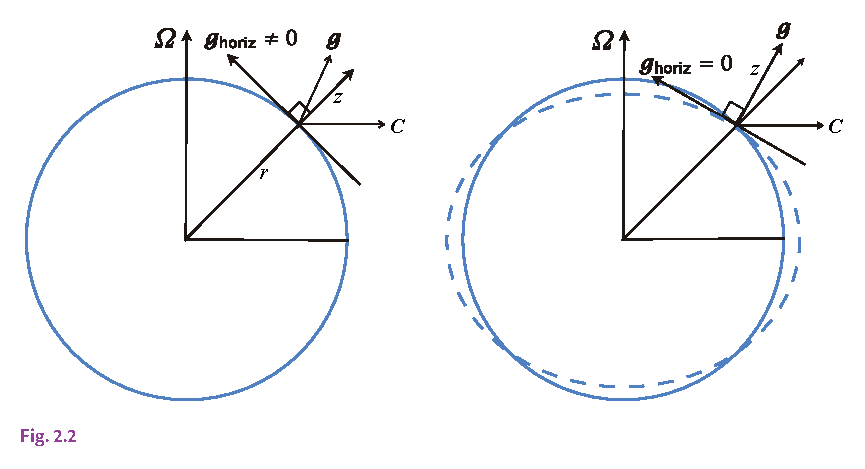
\includegraphics[width=\textwidth]{assets/fig_centrifugal_force.pdf}
  \caption{
    Left: directions of forces and coordinates in true spherical geometry.
    $\mathbf{g}$ is the effective gravity (including the centrifugal force, $\mathbf{C}$)
    and its horizontal component is evidently non-zero.
    Right: a modified coordinate system, in which the vertical direction is
    defined by the direction of $\mathbf{g}$, and so the horizontal component
    of $\mathbf{g}$ is identically zero. The dashed line schematically indicates
    a surface of constant geopotential.
    The differences between the direction of $\mathbf{g}$ and the direction of
    the radial coordinate, and between the sphere and the geopotential surface,
    are much exaggerated and in reality are similar to the thickness of the
    lines themselves.
    This is Fig. 2.2 in AOFD (Vallis, 2017).
  }
  \label{fig:centrifugal_force}
\end{figure}

\subsection{Coriolis force components}

\begin{figure}[h]
  \centering
  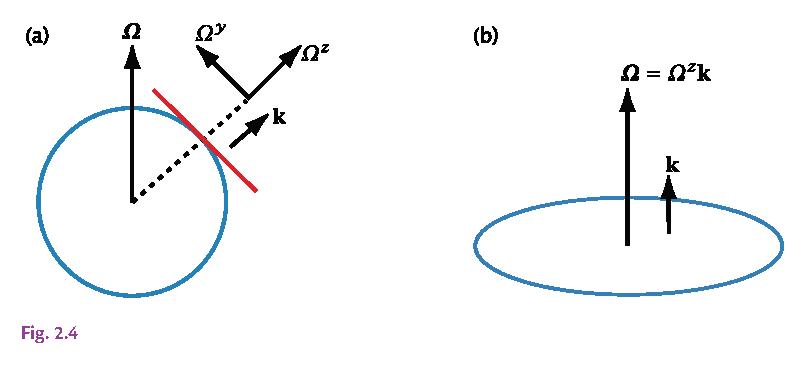
\includegraphics[width=\textwidth]{assets/fig_rotation_components.pdf}
  \caption{
    (a) On the sphere the rotation vector $\mathbf{\Omega}$ can be decomposed
    into two components, one in the local vertical and one in the local horizontal,
    pointing toward the pole. That is, $\mathbf{\Omega} = \Omega_y \mathbf{j} + \Omega_z \mathbf{k}$
    where $\Omega_y = \Omega \cos\theta$ and $\Omega_z = \Omega \sin\theta$.
    In geophysical fluid dynamics, the rotation vector in the local vertical
    is often the more important component in the horizontal momentum equations.
    On a rotating disk, (b), the rotation vector $\mathbf{\Omega}$ is parallel
    to the local vertical $\mathbf{k}$.
    This is Fig. 2.4 in AOFD (Vallis, 2017).
  }
  \label{fig:rotation_components}
\end{figure}

Let's now examine in more detail the effects the Coriolis force on the flow.
The angular velocity $\mathbf{\Omega}$ is a vector that points in the direction
oriented from the center of the Earth toward the North Pole
(see Fig. \ref{fig:rotation_components}).
On the surface of the planet, thus, it has two components: A locally vertical
one, $\Omega_z$, and a meridional one, $\Omega_y$:

\begin{equation}
  \mathbf{\Omega} =
  \begin{bmatrix}
    0 \\
    \Omega_y \\
    \Omega_z
  \end{bmatrix} = 
  \begin{bmatrix}
    0 \\
    \Omega \cos\theta \\
    \Omega \sin\theta
  \end{bmatrix}
\end{equation}
where $\theta$ is the latitude.

The Coriolis force is then:

\begin{equation}
  - 2 \mathbf{\Omega} \times \mathbf{u} =
  \begin{bmatrix}
    \mathbf{i} & \mathbf{j} & \mathbf{k} \\
    0 & - 2 \Omega \cos\theta & - 2 \Omega \sin\theta \\
    u & v & w
  \end{bmatrix} =
  \begin{bmatrix}
    - 2 \Omega w \cos\theta + 2 \Omega v \sin\theta \\
    - 2 \Omega u \sin\theta \\
    2 \Omega u \cos\theta
  \end{bmatrix}
\end{equation}
The Coriolis term thus contributes to all three components of the flow, and
their components vary with latitude.
Let's look at the horizontal components first.
On geophysical scales, generally $w \ll u$ and so the $2 \Omega w \cos\theta$
can often be neglected.
The two dominant horizontal components of the Coriolis force then become
$(-2\Omega v \sin\theta, 2\Omega u \sin\theta)$.
These components are zero at the Equator and increase poleward.
The vertical component, $-2 \Omega u \cos\theta$, can be neglected as well as
its magnitude is very small compared to the other terms in the momentum
equation.

The practical implications of the Coriolis flow is that it deflects it
toward the right on the Northern hemisphere and to the left on the Southern
hemisphere.
Let's now incorporate the Coriolis force components into the vector-component
form of the momentum equation and apply some convenient approximations, namely
the f-plane and the $\beta$-plane approximations.

\subsection{f-plane and $\beta$-plane approximations}

Although geophysical fluids flow on a sphere, the curvature of the surface of
the planet is negligible for many applications.
Here we will make the so-called f-plane approximation in which the flow is
assumed to be on a flat plane tangent to the surface of a curved planet.
The main assumption of the f-plane approximation is that the planet's rotation
exhibits only a locally vertical component anywhere on that planet's surface.
In other words, we'll neglect the horizontal component (\textit{i.e.} $\Omega_y$).
With that assumption, the Coriolis force becomes strictly horizontal:

\begin{equation}
  - 2 \mathbf{\Omega} \times \mathbf{u} =
  \begin{bmatrix}
    2 \Omega v \sin\theta \\
    - 2 \Omega u \sin\theta \\
    0
  \end{bmatrix}
\end{equation}

Let's now define the so-called \textit{Coriolis parameter}\index{Coriolis!parameter}
$f_0 = 2 \Omega_z = 2 \Omega \sin\theta$, so we can write the Coriolis force
more concisely as:

\begin{equation}
  - f_0 \mathbf{k} \times \mathbf{u} =
  \begin{bmatrix}
    f_0 v \\
    - f_0 u \\
    0
  \end{bmatrix}
\end{equation}
The effect of the Coriolis force on the flow is now even more apparent:
A positive meridional flow causes a positive zonal acceleration,
and a positive zonal flow causes a negative meridional acceleration.
The implication of this is that the Coriolis force induces clockwise and
counterclockwise rotations in the Northern and Southern hemispheres,
respectively.

Ignoring viscosity for brevity, we can re-write our system of momentum equations as:

\begin{equation}
  \frac{du}{dt} = - \frac{1}{\rho} \frac{\partial p}{\partial x} + f_0 v
\end{equation}

\begin{equation}
  \frac{dv}{dt} = - \frac{1}{\rho} \frac{\partial p}{\partial y} - f_0 u
\end{equation}

\begin{equation}
  \frac{dw}{dt} = - \frac{1}{\rho} \frac{\partial p}{\partial x} - g
\end{equation}

While on the small plane tangential to the planet's surface the local rotation
may be uniform in space, in reality it does vary with latitude:

\begin{equation}
  f = 2 \Omega \sin\theta \approx 2\Omega \sin\theta_0 + 2\Omega (\theta - \theta_0) \cos\theta_0
\end{equation}
from small deviations in $\theta$.
On a plane, the above can be expressed as:

\begin{equation}
f = f_0 + \beta y
\end{equation}
where $f_0 = 2\Omega \sin\theta_0$ and $\beta = \partial f/\partial y = (2\Omega\cos\theta_0) / R_E$
(where $R_E$ is the radius of the Earth).

\subsection{Geostrophic balance}
\label{sec:geostrophic_balance}

Now that we have incorporated the effects of rotation into our equations of motion,
let's evaluate the scales of the terms in the horizontal momentum equations.
We will start from Eq. \ref{eq:momentum_navier_stokes_rotating}, use the f-plane
notation for the Coriolis term, ignore the viscous terms, and drop the gravity
term as we're looking at the flow in the horizontal plane:

\begin{equation}
  \frac{\partial \mathbf{u}}{\partial t} +
  (\mathbf{u} \cdot \nabla) \mathbf{u} +
  \mathbf{f} \times \mathbf{u} =
  - \frac{1}{\rho} \nabla p
\end{equation}

As we did in Section \ref{sec:nondimensionalization_and_scaling}, let's scale
each term on the left-hand side with their characteristic scales for mesoscale
ocean flow ($L \sim 10^5\ m$, $T \sim 10^6\ s$, $U \sim 10^{-1}\ m/s$):

\begin{itemize}
  \item $\frac{\partial \mathbf{u}}{\partial t} \sim \frac{U}{T} \sim 10^{-7}$
  \item $(\mathbf{u} \cdot \nabla) \mathbf{u} \sim \frac{U^2}{L} \sim 10^{-7}$
  \item $\mathbf{f} \times \mathbf{u} \sim f_0 U \sim 10^{-6}$
\end{itemize}
This means that on these oceanic scales ($L \sim 100\ km$, $T \sim 1\ day$),
the inertial terms are of the same order of magnitude as the Coriolis term.
In other words, rotation here is much more important than the local rate of
change or advection.
Also, whatever the scale of the pressure gradient term is, it is the only
term that can balance the rotation.
Thus, if we can state that the inertial terms can be neglected, we can also
state:

\begin{equation}
  \mathbf{f} \times \mathbf{u} \approx - \frac{1}{\rho} \nabla p
\end{equation}
or, in scalar component form:

\begin{equation}
  f u \approx - \frac{1}{\rho} \frac{\partial p}{\partial y}
\end{equation}

\begin{equation}
  f v \approx \frac{1}{\rho} \frac{\partial p}{\partial x}
\end{equation}

This balance is called the
\textit{geostrophic balance}\index{Geostrophic!balance}\index{Balance!geostrophic},
and it is a key concept in geophysical fluid dynamics.
It states that the flow is governed by the balance between the rotation and the
pressure gradient force.
Although the geostrophic balance is strictly an approximation and it never holds
exactly, large scale oceanic ($L \sim 100\ km$ and larger) and atmospheric
($L \sim 1000\ km$ and larger) flows are often in geostrophic balance.
For the analysis of geophysical flows at such scales, it is then useful to
define the \textit{geostrophic velocity}\index{Geostrophic!velocity} as:

\begin{equation}
  u_g = - \frac{1}{\rho f} \frac{\partial p}{\partial y}
  \label{eq:geostrophic_velocity_u}
\end{equation}

\begin{equation}
  v_g = \frac{1}{\rho f} \frac{\partial p}{\partial x}
  \label{eq:geostrophic_velocity_v}
\end{equation}
Notice that the geostrophic flow is always perpendicular to the pressure gradient,
which means it is parallel to the isobars (lines of constant pressure).
This also means that the isobars are streamlines of the geostrophic flow.
In the northern hemisphere ($f > 0$), the geostrophic flow is cyclonic
(counter-clockwise) around the low-pressure region and anti-cyclonic
(clockwise) around the high-pressure region.
In the southern hemisphere ($f < 0$), it is the opposite.
A nearly geostrophic flow is illustrated in Fig. \ref{fig:geostrophic_flow}.

\begin{figure}[h]
  \centering
  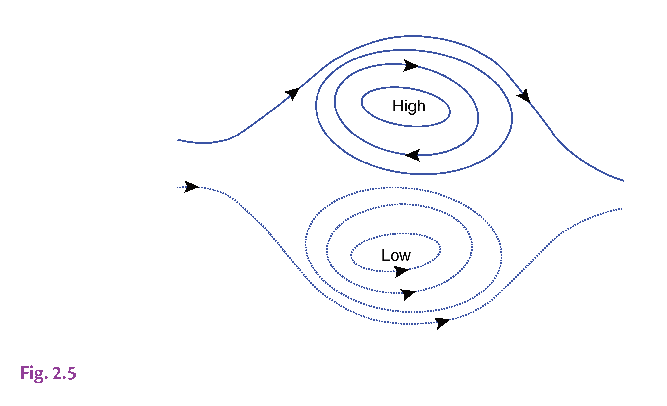
\includegraphics[width=0.8\textwidth]{assets/fig_geostrophic_balance.pdf}
  \caption{
    Geostrophic flow with a positive value of the Coriolis parameter $f$.
    Flow is parallel to the lines of constant pressure (isobars).
    Cyclonic flow is anticlockwise around a low pressure region and
    anticyclonic flow is clockwise around a high. If $f$ were negative, as in
    the Southern Hemisphere, (anti)cyclonic flow would be (anti)clockwise.
    This is Fig. 2.5 in AOFD (Vallis, 2017).
  }
  \label{fig:geostrophic_flow}
\end{figure}

\subsection{Rossby number}

Recall that we required the inertial terms to be much smaller than the Coriolis
term for the geostrophic approximation to hold.
Like we did earlier with the Reynolds number to quantify how turbulent a flow is,
we can define the \textit{Rossby number}\index{Rossby!number} as:

\begin{equation}
  \text{Ro} \equiv
  \frac{\text{Advection}}{\text{Rotation}} = 
  \frac{\left( \mathbf{u} \cdot \nabla \right) \mathbf{u}}{\mathbf{f} \times \mathbf{u}}
  \approx \frac{\frac{U^2}{L}}{fU}
  \approx \frac{U}{fL}
\end{equation}
Though the Rossby number characterizes the relative importance of rotation in
the flow, notice that the rotation term is in the denominator.
The Rossby number is thus small for flows in which rotation dominates over
advection.
In general, flows with a Rossby number of 0.1 or smaller are considered
approximately geostrophically balanced.

\subsection{Inertial oscillations}
\label{sec:inertial_oscillations}

An analytical solution to the linearized horizontal momentum equations with
rotation gives rise to a steady circular motion called the \textit{inertial
oscillation}\index{Inertial!oscillation}.
Start from the linearized horizontal momentum equations with rotation
and with the pressure gradient force neglected:

\begin{equation}
  \frac{\partial \mathbf{u}}{\partial t} + \mathbf{f} \times \mathbf{u} = 0
\end{equation}
In scalar component form, this is:

\begin{equation}
  \frac{\partial u}{\partial t} + f v = 0
  \label{eq:inertial_oscillation_dudt}
\end{equation}

\begin{equation}
  \frac{\partial v}{\partial t} - f u = 0
  \label{eq:inertial_oscillation_dvdt}
\end{equation}
These two equations are linear but coupled, so we need to decouple them
first to obtain the equations with one unknown variable each.
Differentiate each equation with respect to time to get:

\begin{equation}
  \frac{\partial^2 u}{\partial t^2} + f \frac{\partial v}{\partial t} = 0
\end{equation}

\begin{equation}
  \frac{\partial^2 v}{\partial t^2} - f \frac{\partial u}{\partial t} = 0
\end{equation}
and then insert Eqs. (\ref{eq:inertial_oscillation_dudt})-(\ref{eq:inertial_oscillation_dvdt})
into the above to get:

\begin{equation}
  \frac{\partial^2 u}{\partial t^2} + f^2 u = 0
\end{equation}

\begin{equation}
  \frac{\partial^2 v}{\partial t^2} - f^2 v = 0
\end{equation}
The equations are now decoupled and each is a second-order, linear, homogeneous,
ordinary differential equation with constant coefficients.
The general solution to these equations is:

\begin{equation}
  u = A \cos(f t) + B \sin(f t)
\end{equation}

\begin{equation}
  v = C \cos(f t) + D \sin(f t)
\end{equation}
To find the constants $A$, $B$, $C$, and $D$, take the initial conditions for
the velocity to be $\mathbf{u}(t=0) = [u_0, v_0]$.
This results in:

\begin{equation}
  u = u_0 \cos(f t) + v_0 \sin(f t)
  \label{eq:inertial_oscillation_u}
\end{equation}

\begin{equation}
  v = v_0 \cos(f t) - u_0 \sin(f t)
  \label{eq:inertial_oscillation_v}
\end{equation}
These equations describe a circular motion in the horizontal plane with a radius
of $r_0 = \sqrt{u_0^2 + v_0^2} / f$.
It can be demonstrated that the motion is circular by integrating the velocities
(Eqs. \ref{eq:inertial_oscillation_u}-\ref{eq:inertial_oscillation_v}) over time
to obtain displacements $x(t)$ and $y(t)$ and showing that the displacement
radius $r = \sqrt{x^2 + y^2}$ is constant, which can only be true for a circular
motion.

\subsection{Exercises}

\begin{enumerate}
  \item Calculate the effective gravity at the Earth's Equator, poles, and 45 degrees
  latitude, taking into effect centrifugal acceleration.
  \item Using scale analysis, show that on geophysical scales the vertical
  component of the Coriolis force is negligible compared to the other terms
  in the momentum equation.
  \item Derive the Coriolis parameter $f$ on the $\beta$-plane assuming small
  variation in latitude $\theta$ around the constant $\theta_0$ at which $f = f_0$.
\end{enumerate}

\subsection*{Further reading}

\begin{itemize}
  \item Sections 2.1-2.3 and 3.3 of \textit{EAOD} by Vallis
\end{itemize}

\newpage
\section{Stratified flows}

We derived our equations for mass and momentum conservation and we incorporated
the effects of rotation.
We also explored how the density may vary in the vertical according to the
ideas gas law (in the atmosphere) or the equation of state for seawater.
We now explore the effects of stratification on the flow and examine the
common approximations used for large-scale oceanic flows.

\subsection{The Boussinesq equations}

The \textit{Boussinesq approximation}\index{Boussinesq!approximation} is an
approximation to the full equations of motion.
It assumes that the density and pressure perturbations are much smaller than
their means, and when applied to the Navier-Stokes equations, results in the
\textit{Boussinesq equations}\index{Boussinesq!equations}.

We start by decomposing the density and pressure into the mean and the
perturbation components:

\begin{equation}
  \rho = \rho_0 + \delta \rho(x, y, z, t)
  \label{eq:boussinesq_density}
\end{equation}
where $\rho_0$ is the mean density and $\delta \rho$ is its perturbation.
Further, we decompose the pressure as:

\begin{equation}
  p = p_0(z) + \delta p(x, y, z, t)
  \label{eq:boussinesq_pressure}
\end{equation}
where $p_0$ is the horizontally and temporally averaged pressure and $\delta p$
is its perturbation.
Unlike in the density decomposition, the mean pressure component is allowed to
vary in $z$.
For both quantities, we require that their perturbations are much smaller
than their respective means, \textit{i.e.} $\delta \rho \ll \rho_0$, $\delta p \ll p_0$.
In other words, the pressure vary much more in the vertical than in the
horizontal or over time, and any perturbations in density, including those in
the vertical, are much smaller than the mean density.
This approximation can be demonstrated to hold well by using the equation of
state for seawater (Eq. \ref{eq:equation_of_state_ocean}), for example.
The hydrostatic approximation for them is trivially satisfied:

\begin{equation}
  \frac{d p_0}{d z} = - \rho_0 g
  \label{eq:boussinesq_pressure_hydrostatic}
\end{equation}

Now that we've established the approximation we need, let's proceed to apply it
to our momentum and continuity equations.

\subsubsection{Momentum balance}

Let's first apply the Boussinesq approximation to the momentum balance.
Recall the Navier-Stokes equation with rotation
(Eq. \ref{eq:momentum_navier_stokes_rotating}), while neglecting the viscosity
term:

\begin{equation}
  \frac{d \mathbf{u}}{dt} = - \frac{1}{\rho} \nabla p - f \mathbf{k} \times \mathbf{u} + \mathbf{g}
\end{equation}
Apply Eqs. \ref{eq:boussinesq_density}-\ref{eq:boussinesq_pressure} to the
above equation to get:

\begin{equation}
  \left( \rho_0 + \delta \rho \right) \left( \frac{d \mathbf{u}}{dt} + \mathbf{f} \times \mathbf{u} \right) =
  - \nabla \left( p_0 + \delta p \right)
  + \left( \rho_0 + \delta \rho \right) \mathbf{g}
\end{equation}

\begin{equation}
  - \nabla \left( p_0 + \delta p \right) =
  - \nabla \delta p - \frac{\partial p_0}{\partial z} \mathbf{k} = 
  - \nabla \delta p - \rho_0 \mathbf{g}
\end{equation}
Now, recall that $\delta \rho \ll \rho_0$, so we can drop the $\delta \rho$
on the left-hand side:

\begin{equation}
  \rho_0 \left( \frac{d \mathbf{u}}{dt} + \mathbf{f} \times \mathbf{u} \right) =
  - \nabla \delta p + \delta \rho\ \mathbf{g}
\end{equation}

\begin{equation}
  \frac{d \mathbf{u}}{dt} + \mathbf{f} \times \mathbf{u} =
  - \frac{1}{\rho_0} \nabla \delta p + \frac{\delta \rho}{\rho_0} \mathbf{g}
\end{equation}
For convenience of notation, let's now define \textit{buoyancy}\index{buoyancy}
as $b = - g \delta \rho / \rho_0$, and re-write the above to obtain the
Boussinesq momentum equation:

\begin{equation}
  \frac{d \mathbf{u}}{dt} + \mathbf{f} \times \mathbf{u} =
  - \frac{1}{\rho_0} \nabla \delta p + b \mathbf{k}
\end{equation}
This equation states that now that we are in a gradually stratified fluid,
the gravity term is scaled by $\delta \rho / \rho_0$ to yield the appropriate
vertical acceleration, and the pressure gradient is due to the relatively
small perturbations in density $\delta \rho$ around  the mean density $\rho_0$.

\subsubsection{Continuity}

As we did for the momentum equation, we'll now apply the Boussinesq approximation
(\textit{i.e.} $\rho = \rho_0 + \delta \rho$, $\delta \rho \ll \rho_0$) to the
continuity equation.
Recall the continuity equation in its complete form:

\begin{equation}
  \frac{d \rho}{dt} + \rho \nabla \cdot \mathbf{u} = 0
\end{equation}
Insert Eq. \ref{eq:boussinesq_density} to get:

\begin{equation}
  \frac{d\delta \rho}{dt} + \left( \rho_0 + \delta \rho \right) \nabla \cdot \mathbf{u} = 0
\end{equation}
Then, if we can state that that $d\delta \rho / dt \ll \rho_0 \nabla \cdot \mathbf{u}$,
which we will for the Boussinesq approximation, we recover the original
continuity equation for incompressible flows:

\begin{equation}
  \nabla \cdot \mathbf{u} = 0
\end{equation}
Note that we do not say that strictly $d \delta \rho / dt = 0$, but rather that
we can neglect it in this equation in favor of the velocity divergence term.
The evolution of $\delta \rho$ is still governed by the evolution of buoyancy,
which in turn is governed by the evolution of the temperature and salinity fields
and the equation of state.
The buoyancy $b = - g \delta \rho / \rho_0$ evolves as:

\begin{equation}
  \frac{d b}{dt} = \dot{b}
\end{equation}
and the equation of state can be expressed in terms of buoyancy:

\begin{equation}
  b = b(T, S, p)
\end{equation}
which is just another form of Eq. \ref{eq:equation_of_state_ocean}.

Finally the temperature and salinity evolve as before, following
Eqs. \ref{eq:temperature_equation_ocean} and \ref{eq:salinity_equation_ocean},
respectively.

\subsubsection{Complete system of equations}

The full system of Boussinesq equations for the ocean are then:

\begin{equation}
  \frac{d \mathbf{u}}{dt} + \mathbf{f} \times \mathbf{u} =
  - \frac{1}{\rho_0} \nabla \delta p + b \mathbf{k}
\end{equation}

\begin{equation}
  \nabla \cdot \mathbf{u} = 0
\end{equation}

\begin{equation}
  \frac{d T}{dt} = \dot{T}
\end{equation}

\begin{equation}
  \frac{d S}{dt} = \dot{S}
\end{equation}

\begin{equation}
  b = b(T, S, p)
\end{equation}

\subsection{Thermal wind balance}

Now that we regard the ocean as a stratified and rotating fluid with a buoyancy
defined as $b = - g \delta \rho / \rho_0$, an emerging property of the flow
appears if we combine this fact with the geostrophic balance
(see Section \ref{sec:geostrophic_balance}).
Recall the components of geostrophic velocity (Eqs. \ref{eq:geostrophic_u}-\ref{eq:geostrophic_v}):

\begin{equation}
  u_g = - \frac{1}{\rho f} \frac{\partial p}{\partial y}
  \label{eq:geostrophic_u}
\end{equation}

\begin{equation}
  v_g = \frac{1}{\rho f} \frac{\partial p}{\partial x}
  \label{eq:geostrophic_v}
\end{equation}

Differentiate each with respect to $z$ to get:

\begin{equation}
  \frac{\partial u_g}{\partial z} =
  - \frac{1}{\rho f} \frac{\partial^2 p}{\partial z \partial y} =
  - \frac{1}{\rho f} \frac{\partial}{\partial y} \left( \frac{\partial p_0}{\partial z} + \frac{\partial \delta p}{\partial z} \right)
\end{equation}

\begin{equation}
  \frac{\partial v_g}{\partial z} =
  \frac{1}{\rho f} \frac{\partial^2 p}{\partial z \partial x} =
  \frac{1}{\rho f} \frac{\partial}{\partial x} \left( \frac{\partial p_0}{\partial z} + \frac{\partial \delta p}{\partial z} \right)
\end{equation}
Applying the hydrostatic approximation (Eq. \ref{eq:boussinesq_pressure_hydrostatic})
to the above equations, and recalling the definition of buoyancy, we get:

\begin{equation}
  \frac{\partial u_g}{\partial z} =
  - \frac{1}{f} \frac{\partial b}{\partial y}
  \label{eq:thermal_wind_u}
\end{equation}

\begin{equation}
  \frac{\partial v_g}{\partial z} =
  \frac{1}{f} \frac{\partial b}{\partial x}
  \label{eq:thermal_wind_v}
\end{equation}

Equations \ref{eq:thermal_wind_u}-\ref{eq:thermal_wind_v} are known as the
\textit{thermal wind balance}\index{Thermal wind!balance}
(despite the name, it applies to oceans and atmopsheres alike!).
It states that the geostrophic velocity must be vertically sheared in the
presence of a horizontal buoyancy (density) gradient. 
This is illustrated in Fig. \ref{fig:thermal_wind}.

\begin{figure}[h]
  \centering
  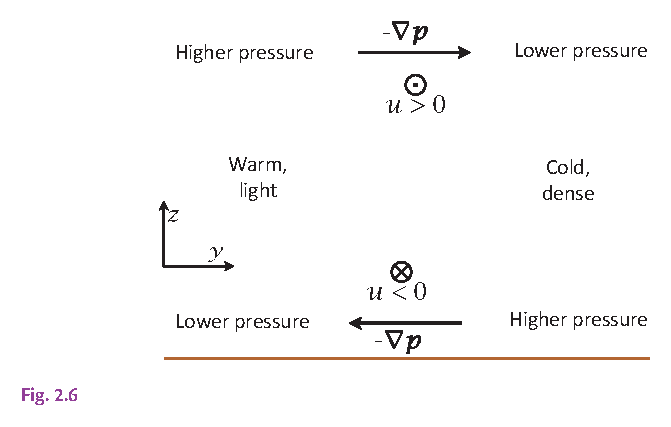
\includegraphics[width=0.8\textwidth]{assets/fig_thermal_wind.pdf}
  \caption{
    The mechanism of thermal wind. A cold fluid is denser than a warm fluid,
    so by hydrostasy the vertical pressure gradient is greater where the fluid
    is cold. Thus, pressure gradients form as shown, where "higher" and "lower"
    mean relative to the average at that height. The horizontal pressure gradients
    are balanced by the Coriolis force, producing (for $f > 0$) the horizontal
    winds shown. Only the wind shear is given by the thermal wind.
    This is Fig. 2.6 in AOFD (Vallis, 2017).
  }
  \label{fig:thermal_wind}
\end{figure}

\subsection{Static instability}

We now consider how a fluid parcel may oscillate when its density is perturbed
from its resting state and in absence of horizontal flow.
This allows us to study the vertical motions due to the vertical differences
in density and in isolation from other processes.
We will approach this problem by displacing a fluid parcel
\textit{adiabatically}\index{adiabatic!displacement}
(i.e. without exchange of heat or mass with the environment) by a small distance
$\delta z$ and examining how the pressure and gravity forces act on it in response
(Fig. \ref{fig:static_instability}).
Recall that in Eq. \ref{eq:boussinesq_density} we allowed for the density
variations to be much smaller than the mean density, \textit{i.e.}
$\delta \rho \ll \rho_0$.
Here we expand the density decomposition to a finer detail, specifically:

\begin{equation}
  \rho = \rho_0 + \widetilde{\rho}(z) + \delta \rho(x, y, z, t)
\end{equation}
where we now differentiate between the mean density $\rho_0$ and the
vertically-varying environmental density $\widetilde{\rho}(z)$, while the 
perturbation $\delta \rho$ includes the vertical, horizontal, and temporal
density variations.

\begin{figure}[h]
  \centering
  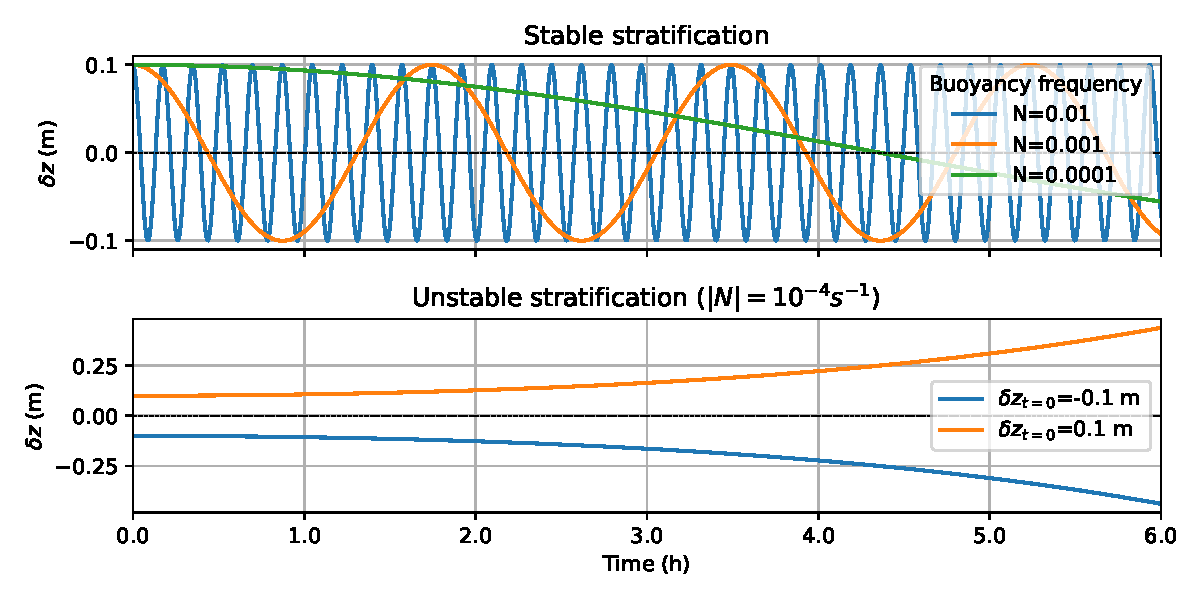
\includegraphics[width=0.8\textwidth]{assets/fig_static_instability.pdf}
  \caption{
    A parcel is adiabatically displaced upward from level $z$ to $z + \delta z$.
    A tilde denotes the value in the environment, and variables without tildes
    are those in the parcel.
    The parcel preserves its potential density, $\rho_\theta$, which it takes
    from the environment at level $z$.
    If $z + \delta z$ is the reference level, the potential density there is
    equal to the actual density.
    The parcel's stability is determined by the difference between its density
    and the environmental density.
    If the difference is positive, the displacement is stable, and if negative
    the displacement is unstable.
    This is Fig. 2.8 in AOFD (Vallis, 2017).
  }
  \label{fig:static_instability}
\end{figure}

As the fluid parcel is displaced adiabatically, its pressure changes
instantaneously to assume the same pressure as the environment.
However, its temperature and salinity do not change instantaneously, resulting
in a density change.
To account for the instantaneous change in pressure as the parcel is displaced
in height, rather than the actual density we need to consider the parcel's
\textit{potential density}\index{Potential density}, $\rho_\theta$.
The potential density is the density the parcel would have if it were returned
to the level where the initial pressure was $p_0$:

\begin{equation}
  \rho_\theta = \rho + \frac{p_0}{c_s^2} = \rho + \frac{\rho_0 g z}{c_s^2}
  \label{eq:potential_density}
\end{equation}
where $c_s^2 = \left| \partial p / \partial \rho \right|_\theta$ is the square of
the speed of sound in the fluid, which we here assume to be constant and equal
to $\approx 1500 \, \text{m/s}$.
$c_s^2$ is also related to the pressure compressibility of the fluid in the
equation of state for seawater (Eq. \ref{eq:equation_of_state_ocean}),
$\beta_p = 1/(\rho_0 c_s^2)$.
Thus, if the parcel ascends or descends adiabatically, without a change in
temperature or salinity, but allowing it to assume environmental pressure,
its density will change but its potential density will remain constant.
Potential density is thus a useful concept for understanding the static stability
of the fluid.

From Fig. \ref{fig:static_instability}, taking the reference level to be 
$z + \delta z$, we have:

\begin{equation}
  \delta \rho = \rho(z + \delta z) - \widetilde{\rho}(z + \delta z) =
  \rho_\theta(z + \delta z) - \widetilde{\rho}_\theta(z + \delta z) =
  \widetilde{\rho}_\theta(z) - \widetilde{\rho}_\theta(z + \delta z)  
\end{equation}

Then, for small $\delta z$:

\begin{equation}
  \delta \rho = - \frac{\partial \widetilde{\rho}_\theta}{\partial z} \delta z
\end{equation}

The parcel's static stability is thus determined by the vertical gradient of
the locally-referenced potential density of the environment,
$\widetilde{\rho_\theta}$:

\begin{equation}
  \frac{\partial \widetilde{\rho}_\theta}{\partial z} < 0 \quad \text{(statically stable)}
\end{equation}

\begin{equation}
  \frac{\partial \widetilde{\rho}_\theta}{\partial z} > 0 \quad \text{(statically unstable)}
\end{equation}

Now, to determine the oscillatory motion of the parcel, we apply Newton's second
law and balance the acceleration of the parcel with the buoyancy force:

\begin{equation}
  \frac{\partial^2 \delta z}{\partial t^2} = \frac{g}{\rho} \left( \frac{\partial \widetilde{\rho}_\theta}{\partial z} \right) \delta z =
  - N^2 \delta z
\end{equation}
where we have defined the \textit{Brunt-Väisälä frequency}\index{Brunt-Väisälä frequency}
(or buoyancy frequency) as:

\begin{equation}
  N^2 = - \frac{g}{\widetilde{\rho}_\theta} \frac{\partial \widetilde{\rho}_\theta}{\partial z} =
  \frac{d\widetilde{b}}{dz}
\end{equation}
while noting that $\rho(z) = \widetilde{\rho}_\theta(z)$ within
$\mathcal{O}(\delta z)$.
A parcel displaced from its equilibrium position will oscillate with angular
frequency $N$ if $N^2 > 0$ (statically stable) and will freely accelerate
upward if $N^2 < 0$ (statically unstable).

\subsection{Exercises}

\begin{enumerate}
  \item Use the linear equation of state for seawater to demonstrate that the
  variations of density in the ocean are very small compared to the mean
  density. How large (in percent relative change) are these variations with
  respect to the changes in temperature, salinity, and pressure in the ocean?
\end{enumerate}

\subsection*{Further reading}

\begin{itemize}
  \item Chapters 2 and 3 of \textit{EAOD} by Vallis
\end{itemize}

\newpage
\section{Shallow water systems}
\label{sec:shallow_water_systems}

In this chapter we move away from the continuously stratified ocean and
approximate it to a single layer of incompressible fluid that is also in
hydrostatic balance.
It turns out that this seemingly drastic approximation still allows the
reduced equation set to reproduce many observed large scale oceanic and
atmospheric phenomena.
In fact, the shallow water system of equations is the basis for some operational
ocean prediction models, especially if applied to the nearshore and coastal
ocean.
We begin by introducing the key assumptions that allow the derivation of the
shallow water equations, and after that we derive the general solutions to the
equations.

\subsection{Key assumptions}

The name "shallow water" may be revealing about the approximations that we will
make about the flow:

\begin{enumerate}
  \item \textbf{Shallow:} The vertical scale of the flow is much smaller than the
    horizontal scale. Although this doesn't mean that there is no vertical
    flow, it does mean that the horizontal flow is much larger,
    \textit{i.e.} $u, v \gg w$.
  \item \textbf{Water:} The flow is incompressible, \textit{i.e.}
  $\nabla \cdot \mathbf{u} = 0$.
\end{enumerate}
As a consequence of the above approximations, our flow will also be hydrostatic,
\textit{i.e.} $\partial p / \partial z = -\rho g$.
This approximation will show to be instrumental in allowing us to cast the 
horizontal pressure gradient in terms of the surface elevation only.

The flow can then be described as a thin layer of fluid over a rigid bottom
that may vary in the horizontal, and with a free surface that can freely
move in the vertical in response to the flow and incompressibility
(Fig. \ref{fig:shallow_water1}).
This layer of fluid may or may not be covered on top by another layer of fluid,
with its own hydrostatic pressure imposed on the surface.

\begin{figure}[h]
  \centering
  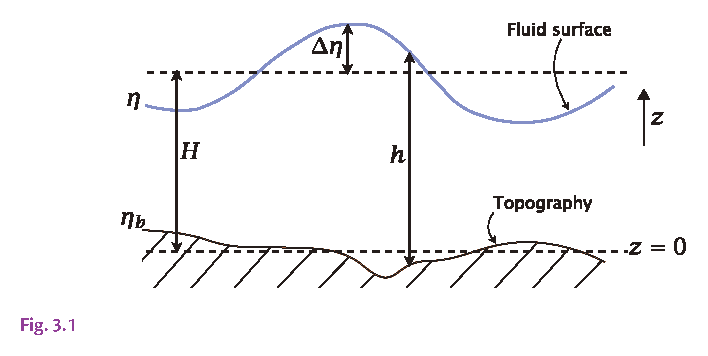
\includegraphics[width=0.8\textwidth]{assets/fig_shallow_water1.pdf}
  \caption{
    A shallow water system.
    $h$ is the thickness of a water column, $H$ its mean thickness, $\eta$ the
    height of the free surface and $\eta_b$ is the height of the lower, rigid
    surface above some arbitrary origin, typically chosen such that the average
    of $\eta_b$ is zero.
    $\Delta \eta$ is the deviation free surface height, so we have
    $\eta = \eta_b + h = H + \Delta \eta$.
    This is Fig. 3.1 in AOFD (Vallis, 2017).
  }
  \label{fig:shallow_water1}
\end{figure}

\subsection{Shallow water equations}

The shallow water equations consist of the momentum and the continuity
equations.
For 2-dimensional horizontal flow, the momentum equation can be expressed as
a single equation in vector form, or as two scalar equations in $x$ and $y$.

\subsubsection{Momentum equation}

We begin from the vector momentum equation with rotation:

\begin{equation}
  \frac{d \mathbf{u}}{dt} + \mathbf{f} \times \mathbf{u} =
  - \frac{1}{\rho} \nabla p + \mathbf{g}
  \label{eq:shallow_water_momentum1}
\end{equation}
In the vertical component of this equation we will neglect the vertical
acceleration to obtain the hydrostatic balance, as we did previously:

\begin{equation}
  \frac{\partial p}{\partial z} = -\rho g
\end{equation}
We can integrate the hydrostatic balance in $z$ to obtain the pressure as a
function of height:

\begin{equation}
  \int_{p(z)}^{p_\eta} dp = - \int_z^\eta \rho g \, dz
\end{equation}
where $p_\eta$ is the pressure at $z = \eta$.
Rearranging the terms after integration yields:

\begin{equation}
  p(z) = p_\eta + \rho g \eta - \rho g z
\end{equation}
We will now take a horizontal gradient to both sides and assume for simplicity
that the horizontal gradient of $p_\eta$ is negligible compared to the other
terms.
Further, taking that neither the density nor gravity vary in the horizontal,
and noting that $z$ as a vertical coordinate cannot vary in the horizontal,
we get:

\begin{equation}
  \nabla p = \rho g \nabla \eta
  \label{eq:shallow_water_momentum2}
\end{equation}
Inserting Eq. \ref{eq:shallow_water_momentum2} into
Eq. \ref{eq:shallow_water_momentum1}, and taking $\nabla$ to be the horizontal
divergence going forward, we get:

\begin{equation}
  \frac{d \mathbf{u}}{dt} + \mathbf{f} \times \mathbf{u} =
  - g \nabla \eta
  \label{eq:shallow_water_momentum3}
\end{equation}
which is the horizontal shallow water momentum equation with rotation.
Let's now proceed to derive the shallow water continuity equation and complete
the system of equations.

\subsubsection{Continuity equation}

An intuitive approach to deriving the shallow water continuity is to consider
a column of fluid in a one-dimensional horizontal flow whose spatial variations
would cause a change in the surface elevation of that column due to the
incompressibility (Fig. \ref{fig:shallow_water2}).
Although the bottom surface here is shown to be flat, recall from Fig.
\ref{fig:shallow_water1} that it doesn't need to be, and the water column height
$h$ comprises of the water depth (as measured from the rigid bottom to the mean
water level) plus the deviation of the free surface from the mean water level,
$\Delta \eta$.

\begin{figure}[h]
  \centering
  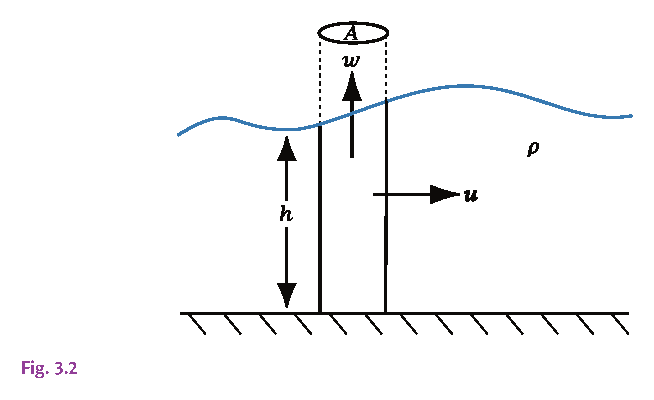
\includegraphics[width=0.8\textwidth]{assets/fig_shallow_water2.pdf}
  \caption{
    The mass budget for a column of area $A$ in a shallow water system.
    There is a non-zero vertical velocity at the top of the column if the mass
    convergence into the column is non-zero.
    This is Fig. 3.2 in AOFD (Vallis, 2017).
  }
  \label{fig:shallow_water2}
\end{figure}

The difference between the amount of liquid flowing into and out of the column
thus must be balanced by a change in the surface elevation of the column:

\begin{equation}
  u_2 h_2 - u_1 h_1 = \frac{\partial \eta}{\partial t} \Delta x
\end{equation}
Rearranging the terms leads to:

\begin{equation}
  \frac{\partial \eta}{\partial t} = 
  \frac{u_2 h_2 - u_1 h_1}{\Delta x} \approx
  \frac{\partial (u h)}{\partial x}
  \label{eq:shallow_water_continuity1}
\end{equation}
Generalized in vector form, this becomes the Eulerian form of the shallow water
continuity equation:

\begin{equation}
  \frac{\partial \eta}{\partial t} + \nabla \cdot (h \mathbf{u}) = 0
  \label{eq:shallow_water_continuity2}
\end{equation}
and from there, while noting that $h - \eta$, the mean water depth, does not vary
in time, the Lagrangian form is:

\begin{equation}
  \frac{d \eta}{dt} + h \nabla \cdot \mathbf{u} = 0
  \label{eq:shallow_water_continuity3}
\end{equation}

Alternatively, we can derive the shallow water continuity from the incompressibility
of the flow:

\begin{equation}
  \nabla \cdot \mathbf{u} = 
  \frac{\partial u}{\partial x} + 
  \frac{\partial v}{\partial y} + 
  \frac{\partial w}{\partial z} = 0
\end{equation}

\begin{equation}
  \frac{\partial w}{\partial z} \approx \frac{w_\eta - w_b}{h} = - \frac{\partial u}{\partial x} - \frac{\partial v}{\partial y}
\end{equation}
where $w_\eta$ and $w_b$ are the vertical velocities at the free surface and the
rigid bottom surface, respectively, and $h$ is, again, the distance of the free
surface from the bottom.
$w_b$ must be zero, of course, and $w_\eta = \partial \eta / \partial t$,
so we get:

\begin{equation}
  \frac{d \eta}{dt} + h \nabla \cdot \mathbf{u} = 0
\end{equation}
which is the Lagrangian form of the shallow water continuity and the same
equation as Eq. \ref{eq:shallow_water_continuity3}.
To get the Eulerian form from here, we first need to recognize that
$d\eta/dt = dh/dt$ because $h = \overline{h} + \eta$, where $\overline{h}$ is the
mean water depth.
Then, expanding the Lagrangian derivative, we recover Eq.
\ref{eq:shallow_water_continuity2}.

\subsubsection{The complete equation set}

The momentum and continuity equations that we derived above form the complete
set of shallow water equations.
In vector form, they are:

\begin{equation}
  \frac{d \mathbf{u}}{dt} + \mathbf{f} \times \mathbf{u} =
  - g \nabla \eta
  \label{eq:shallow_water_final_momentum}
\end{equation}

\begin{equation}
  \frac{\partial \eta}{\partial t} + \nabla \cdot (h \mathbf{u}) = 0
  \label{eq:shallow_water_final_continuity}
\end{equation}

And in scalar form, in two dimensions:

\begin{equation}
  \frac{\partial u}{\partial t} +
  u \frac{\partial u}{\partial x} +
  v \frac{\partial u}{\partial y} -
  f v = 
  -g \frac{\partial \eta}{\partial x}
  \label{eq:shallow_water_final_scalar_u}
\end{equation}

\begin{equation}
  \frac{\partial v}{\partial t} +
  u \frac{\partial v}{\partial x} +
  v \frac{\partial v}{\partial y} +
  f u =
  -g \frac{\partial \eta}{\partial y}
  \label{eq:shallow_water_final_scalar_v}
\end{equation}

\begin{equation}
  \frac{\partial \eta}{\partial t} +
  \frac{\partial (hu)}{\partial x} +
  \frac{\partial (hv)}{\partial y} = 0
  \label{eq:shallow_water_final_scalar_eta}
\end{equation}
which closes our system of equations.
In two dimensions, we thus have three equations for the three unknown
variables $u$, $v$, and $\eta$.
The flow is inviscid (no friction) but nonlinear (advective term
$\mathbf{u} \cdot \nabla \mathbf{u}$ is present), so this system of equations
allows for turbulence but does not dissipate energy.
Also, notice that the Coriolis force is present but has seamlessly percolated
from the starting equation without breaking any of the assumptions.
Thus, to consider shallow water systems in a non-rotating frame, simply drop
the Coriolis term.

We now proceed to further simplify this equation set to derive a general
solution for the shallow water equations.

\subsection{Poincaré waves}
\label{sec:poincare_waves}

As we proceed without our intention to derive a solution to the
equations (\ref{eq:shallow_water_final_scalar_u}-\ref{eq:shallow_water_final_scalar_eta}),
notice that the nonlinear terms get in the way of an analytical solution.
To work around this, we will linearize the equations by decomposing the flow
into a mean and a perturbation:

\begin{equation}
  h(x, y, t) = H + \eta'(x, y, t)
\end{equation}

\begin{equation}
  \mathbf{u}(x, y, t) = \mathbf{U} + \mathbf{u}'(x, y, t)
\end{equation}
and since the mean flow in space and time does not vary, and it is by definition
zero for the fluid at rest, then the velocity field is equal to its perturbation:

\begin{equation}
  \mathbf{u}(x, y, t) = \mathbf{u}'(x, y, t)
\end{equation}

Insert these decompositions Eqs. (\ref{eq:shallow_water_final_momentum})
and (\ref{eq:shallow_water_final_continuity}) to get:

\begin{equation}
  \frac{\partial \mathbf{u}'}{\partial t} + 
  \mathbf{u}' \cdot \nabla \mathbf{u}' +
  \mathbf{f} \times \mathbf{u}' =
  - g \nabla \left( H + \eta' \right)
\end{equation}

\begin{equation}
  \frac{\partial \eta'}{\partial t} + \nabla \cdot \left[ (H + \eta') \mathbf{u}' \right] = 0
\end{equation}
Although we do not (and cannot) require that the perturbations on their own
are small enough to neglect, the products of two perturbations are assumed to
be.
This allows us to linearize the equations and obtain:

\begin{equation}
  \frac{\partial \mathbf{u}'}{\partial t} + 
  \mathbf{f} \times \mathbf{u}' +
  g \nabla \eta' = 0
\end{equation}

\begin{equation}
  \frac{\partial \eta'}{\partial t} + H \nabla \cdot \mathbf{u}' = 0
\end{equation}
Or, in scalar form:

\begin{equation}
  \frac{\partial u'}{\partial t} - f v' + g \frac{\partial \eta'}{\partial x} = 0
  \label{eq:swe_linear_u}
\end{equation}

\begin{equation}
  \frac{\partial v'}{\partial t} + f u' + g \frac{\partial \eta'}{\partial y} = 0
  \label{eq:swe_linear_v}
\end{equation}

\begin{equation}
  \frac{\partial \eta'}{\partial t} + H \frac{\partial u'}{\partial x} + H \frac{\partial v'}{\partial y} = 0
  \label{eq:swe_linear_eta}
\end{equation}

Assume the general solution to have a wave-like form:

\begin{equation}
  (u, v, \eta) = (\widehat{u}, \widehat{v}, \widehat{\eta}) e^{i(kx + ly - \omega t)}
\end{equation}
where $\widehat{u}$, $\widehat{v}$, and $\widehat{\eta}$ are the amplitudes of the
wave-like perturbations, $k$ and $l$ are the wavenumbers, and $\omega$ is the
angular frequency.
Insert the wave form into Eqs. (\ref{eq:swe_linear_u}-\ref{eq:swe_linear_eta})
to get:

\begin{equation}
  - i \omega \widehat{u} - f \widehat{v} + i g k \widehat{\eta} = 0
\end{equation}

\begin{equation}
  - i \omega \widehat{v} + f \widehat{u} + i g l \widehat{\eta} = 0
\end{equation}

\begin{equation}
  - i \omega \widehat{\eta} + i H k \widehat{u} + i H l \widehat{v} = 0
\end{equation}
or, in matrix form:

\begin{equation}
  \begin{bmatrix}
    - i \omega & - f        & i g k \\
    f          & - i \omega & i g l \\
    i H k      & i H l      & - i \omega
  \end{bmatrix}
  \begin{bmatrix}
    \widehat{u} \\
    \widehat{v} \\
    \widehat{\eta}
  \end{bmatrix} = 0
\end{equation}
The solution to this system requires that the determinant of the matrix be zero,
which yields:

\begin{equation}
  \omega[\omega^2 - f^2 - gH(k^2 + l^2)] = 0
  \label{eq:swe_determinant}
\end{equation}
A trivial solution to this equation is $\omega = 0$, which corresponds to an
unperturbed, constant flow.
The other, non-trivial solution is the dispersion relation for shallow water
gravity waves in a rotating frame:

\begin{equation}
  \omega = \sqrt{f^2 + gH(k^2 + l^2)}
  \label{eq:swe_dispersion}
\end{equation}
This dispersion relationship connects the frequency to the wavenumber, and we
see that it scales with the Coriolis frequency $f$ and the gravity wave
phase speed $\sqrt{gH}$.
This general solution corresponds to the so-called
\textit{Poincaré waves}\index{Poincaré waves}, which are the surface gravity
waves with effects of rotation.
They are also commonly referred to as
\textit{inertial-gravity waves}\index{Inertial-gravity waves}.
Increasing the Coriolis parameter $f$ while keeping the other parameters fixed
increases the frequency of the waves by enhancing the rotation.
Similarly, increasing the gravitational acceleration $g$ or the mean water depth
$H$ increases the frequency of the waves by enhancing the gravity wave phase
speed.
Notice also that the frequency $\omega$ scales linearly with the wavenumber
$k^2 + l^2$, their ratio $\omega / (k^2 + l^2)$ being the phase speed of the
wave:

\begin{equation}
  c_p = \frac{\omega}{\sqrt{k^2 + l^2}} = \sqrt{\frac{f^2}{k^2 + l^2} + gH}
\end{equation}

\begin{figure}[h]
  \centering
  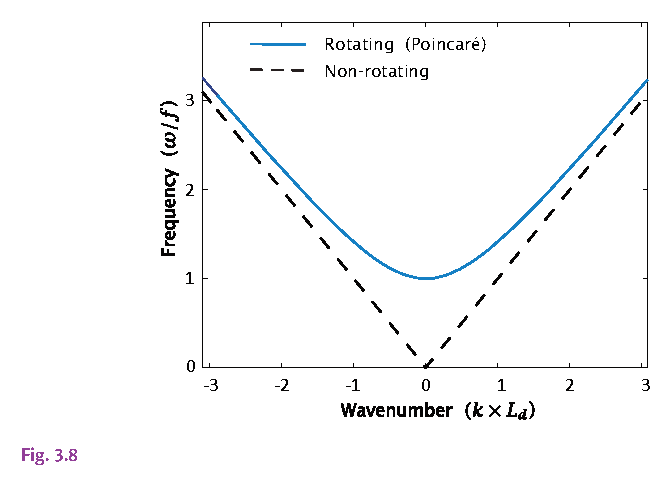
\includegraphics[width=0.8\textwidth]{assets/fig_swe_dispersion.pdf}
  \caption{
    Dispersion relation for Poincaré waves and non-rotating shallow water
    waves.
    Frequency is scaled by the Coriolis frequency $f$, and wavenumber by the
    inverse deformation radius $\sqrt{gH}/f$.
    For small wavenumbers the frequency of the Poincaré waves is approximately
    $f$, and for high wavenumbers is asymptotes to that of non-rotating waves.
    This is Fig. 3.8 in AOFD (Vallis, 2017).
  }
  \label{fig:swe_dispersion}
\end{figure}

As there are two independent parameters in Eq. \ref{eq:swe_dispersion} that
originate from different terms in the shallow water equations, we can turn the
knobs on each to explore some limiting cases of the general solution.

\subsubsection{Short gravity waves}

In the case of short gravity waves, the pressure gradient terms (and thus,
gravity) dominate the Coriolis term (rotation):

\begin{equation}
  gH(k^2 + l^2) \gg f^2
\end{equation}
In this case, the dispersion relation simplifies to:

\begin{equation}
  \omega = \sqrt{gH(k^2 + l^2)}
\end{equation}
which is the dispersion relation for (non-rotating) shallow water gravity waves.
Notice, however, that we don't require there to be no rotation at all to obtain
the non-rotating gravity waves.
Rather, we simply require that the waves are so short (high wavenumber) that the
Coriolis force is negligible compared to the gravity force.
Real-life examples of this solution include tsunamis, wind-generated swell
waves on the ocean surface, or small ripples that propagate radially outward
when throwing a stone into a pond.

\subsubsection{Inertial oscillations}
\index{Inertial!oscillation}

If the wavenumber is so small (large wavelength) that the gravity term can be
neglected in favor of the Coriolis term, we recover a class of motion that we
explored earlier, the inertial oscillations.
In this case, the rotation dominates over the gravity:

\begin{equation}
  f^2 \gg gH(k^2 + l^2)
\end{equation}
and the dispersion relation simplifies to:

\begin{equation}
  \omega = f
\end{equation}
which corresponds to a circular motion with the frequency that exactly equals
the Coriolis frequency (because $(u, v) = (\widehat{u}, \widehat{v}) e^{- i f t}$).
Recall that we already explored this solution by dropping the pressure gradient
terms in the rotating momentum equations back in Section
\ref{sec:inertial_oscillations}.
Here, it comes out as a limiting case from the general solution which we
couldn't obtain prior to the shallow water approximations and linearization.

\subsection{Kelvin waves}

A special case of the general solution that is particularly relevant to the
atmospheric and oceanic dynamics is that of a linearized shallow water flow
that is bounded on one side by a solid boundary, such as a coastline.
The resulting solution is a special class of gravity waves called
\textit{Kelvin waves}\index{Kelvin waves}, which propagate as a shallow water
gravity wave along the solid boundary and whose propagation direction, as well
as the perturbation scale in the direction away from the boundary, are governed
by the planetary rotation rate.
Kelvin waves appear in both the atmosphere and the ocean.

To derive the Kelvin waves, we start from the linearized shallow water equations
(where we drop the primes for brevity):

\begin{equation}
  \frac{\partial u}{\partial t} - f v = - g \frac{\partial \eta}{\partial x}
\end{equation}

\begin{equation}
  \frac{\partial v}{\partial t} + f u = - g \frac{\partial \eta}{\partial y}
\end{equation}

\begin{equation}
  \frac{\partial \eta}{\partial t} + H \left( \frac{\partial u}{\partial x} + \frac{\partial v}{\partial y} \right) = 0
\end{equation}
Now, suppose that our solid boundary is along the $x$-axis at $y = 0$, which
allows us to neglect the meridional flow ($v=0$):

\begin{equation}
  \frac{\partial u}{\partial t} = - g \frac{\partial \eta}{\partial x}
  \label{eq:kelvin_u}
\end{equation}

\begin{equation}
  f u = - g \frac{\partial \eta}{\partial x}
  \label{eq:kelvin_v}
\end{equation}

\begin{equation}
  \frac{\partial \eta}{\partial t} + H \frac{\partial u}{\partial x} = 0
  \label{eq:kelvin_eta}
\end{equation}
Differentiate Eq. \ref{eq:kelvin_u} with respect to time and Eq. \ref{eq:kelvin_eta}
with respect to $x$, and combine them to get:

\begin{equation}
  \frac{\partial^2 u}{\partial t^2} - gH \frac{\partial^2 u}{\partial x^2} = 0
\end{equation}
which is the standard wave equation, whose solution is a wave that propagates
with the phase speed $c = \sqrt{gH}$.
We will thus assume a wave-like solution for $u$, like we did for the Poincaré
waves in Section \ref{sec:poincare_waves}.
However, since we now have a solid boundary at $y = 0$, we should also assume
that the solution should vary in the $y$ direction (because it must be zero
at the boundary, and non-zero elsewhere).
The general solution for $u$ may be:

\begin{equation}
  u = \widehat{u}(y) e^{i(k - c t)}
  \label{eq:kelvin_u_sol}
\end{equation}
As for the elevation $\eta$, insert Eq. \ref{eq:kelvin_u_sol} into Eq.
\ref{eq:kelvin_eta} to get:

\begin{equation}
  \eta = \sqrt{\frac{g}{H}} \widehat{u}(y) e^{i(k - c t)}
  \label{eq:kelvin_eta_sol}
\end{equation}
We still need to solve for $\widehat{u}(y)$, so we look for the equation that
has a derivative with respect to $y$.
So, insert Eqs. \ref{eq:kelvin_u_sol} and \ref{eq:kelvin_eta_sol} into Eq.
\ref{eq:kelvin_v} to get:

\begin{equation}
  f \widehat{u}(y) = - \sqrt{\frac{H}{g}} \frac{\partial \widehat{u}(y)}{\partial y}
\end{equation}
which integrates to:

\begin{equation}
  \widehat{u}(y) = \widehat{u}_0 e^{-\frac{y}{L_d}}
  \label{eq:kelvin_u_sol_y}
\end{equation}
where

\begin{equation}
  L_d = \frac{\sqrt{gH}}{f}
  \label{eq:rossby_deformation_radius}
\end{equation}
is the \textit{Rossby radius of deformation}\index{deformation!Rossby radius}
\index{Rossby!radius of deformation},
which is the length scale at which planetary rotation becomes important
relative to the effects of gravity (or buoyancy, in stratified flows).
The complete solutions for the shallow water Kelvin waves are then:

\begin{equation}
  u = \widehat{u}_0 e^{-\frac{y}{L_d}} e^{i(k - c t)}
\end{equation}

\begin{equation}
  \eta = \sqrt{\frac{H}{g}} \widehat{u}_0 e^{-\frac{y}{L_d}} e^{i(k - c t)}
\end{equation}

\begin{figure}[h]
  \centering
  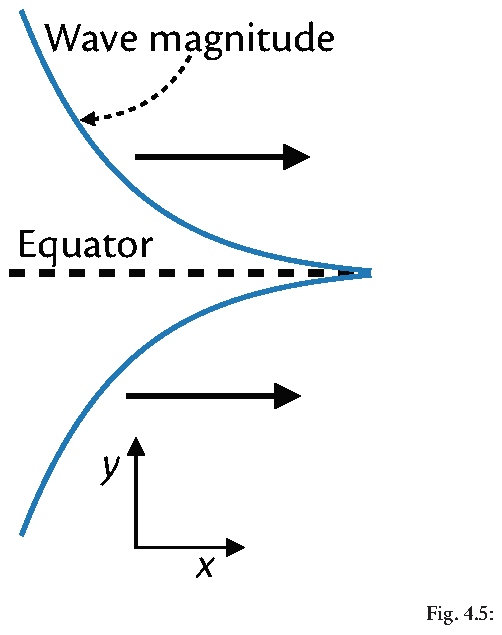
\includegraphics[width=0.4\textwidth]{assets/fig_kelvin_wave.pdf}
  \caption{
    Kelvin waves propagating eastward along the equator and decaying rapidly
    away to either side.
    This is Fig. 4.5 in Vallis (EAOD).
  }
\end{figure}

\subsection{Conservative properties}

We now look at some conservative properties of the shallow water equations,
namely the potential vorticity conservation and the conservation of energy.
The former is a material conservative property, meaning that it is conserved
along a fluid parcel as it moves and deforms.
The latter is a volume-integrated conservative property, meaning that it is
conserved in a control volume as the fluid evolves in time.
The conservation of potential vorticity yields some interesting emerging
properties of the flow, such as the vortex stretching due to the change in the
fluid depth, and the planetary waves due to the meridional variation of the
planetary vorticity (Coriolis parameter $f$).

\subsubsection{Potential vorticity}

\textit{Potential vorticity} (PV)\index{Potential vorticity} describes the rate
of rotation of a fluid parcel scaled by the fluid depth.
It is a material property, meaning that it is conserved along a fluid parcel
as it moves and deforms.
Start from the momentum equation with effects of rotation:

\begin{equation}
  \frac{\partial \mathbf{u}}{\partial t} +
  \mathbf{u} \cdot \nabla \mathbf{u} +
  \mathbf{f} \times \mathbf{u} =
  - g \nabla \eta
\end{equation}
We will rely on the following vector identity to rewrite the advective term:

\begin{equation}
  \mathbf{u} \cdot \nabla \mathbf{u} =
  \frac{1}{2} \nabla (\mathbf{u}^2) -
  \mathbf{u} \times (\nabla \times \mathbf{u})
\end{equation}
and recognize $\nabla \times \mathbf{u} = \boldsymbol{\omega}$ as the vorticity
to rewrite the above as:

\begin{equation}
  \frac{\partial \mathbf{u}}{\partial t} +
  \left(\boldsymbol{\omega} + \mathbf{f}\right) \times \mathbf{u} =
  - g \nabla \left(\eta + \frac{1}{2} \mathbf{u}^2 \right)
\end{equation}
Take a curl of this equation to get:

\begin{equation}
  \frac{\partial (\nabla \times \mathbf{u})}{\partial t} +
  \nabla \times \left[(\boldsymbol{\omega} + \mathbf{f}) \times \mathbf{u}\right] =
  - \nabla \times \nabla \left(\eta + \frac{1}{2} \mathbf{u}^2 \right)
\end{equation}
Next, we use the vector triple product identity:

\begin{equation}
  \nabla \times \boldsymbol{\omega} \times \mathbf{u} =
  (\mathbf{u} \cdot \nabla) \boldsymbol{\omega} -
  (\boldsymbol{\omega} \cdot \nabla) \mathbf{u} +
  \boldsymbol{\omega} \nabla \cdot \mathbf{u} -
  \mathbf{u} \nabla \cdot \boldsymbol{\omega}
\end{equation}
Since vorticity must be divergence free ($\nabla \cdot \boldsymbol{\omega} = 0$),
and it's perpendicular to the velocity vector ($\boldsymbol{\omega} \cdot \mathbf{u} = 0$),
the second and the fourth terms vanish.
Define the vertical component of the vorticity to be:

\begin{equation}
  \zeta = \mathbf{k} \cdot \boldsymbol{\omega}
\end{equation}
to get:

\begin{equation}
  \frac{\partial \zeta}{\partial t} +
  \left(\mathbf{u} \cdot \nabla \right) \left(\zeta + f\right) =
  - \left(\zeta + f\right) \nabla \cdot \mathbf{u}
\end{equation}
Recall the continuity equation:

\begin{equation}
  \frac{dh}{dt} = -h \nabla \cdot \mathbf{u}
\end{equation}
Multiply both sides by $(\zeta + f)$ to write:

\begin{equation}
  \frac{dh}{dt} \frac{\zeta + f}{h} = - \left(\zeta + f\right) \nabla \cdot \mathbf{u}
\end{equation}

\begin{equation}
  \frac{d(\zeta + f)}{dt} = \frac{\zeta + f}{h} \frac{dh}{dt}
\end{equation}
Then, notice that:

\begin{equation}
  \frac{d}{dt} \left( \frac{\zeta}{h} \right) =
  \frac{1}{h} \frac{d\zeta}{dt} +
  \zeta \frac{d}{dt} \left( \frac{1}{h} \right) =
  \frac{1}{h} \frac{d\zeta}{dt} -
  \frac{\zeta}{h^2} \frac{dh}{dt} =
  \frac{1}{h} \left( \frac{d\zeta}{dt} - \frac{\zeta}{h} \frac{dh}{dt} \right)
\end{equation}
which leads to:

\begin{equation}
  \frac{d}{dt} \left( \frac{\zeta + f}{h} \right) = 0
  \label{eq:swe_potential_vorticity}
\end{equation}
where $(\zeta + f)/h$ is the \textit{potential vorticity}\index{Potential vorticity},
and Eq. \ref{eq:swe_potential_vorticity} is the conservation of potential
vorticity.

Let's consider some implications of it.
First, without planetary rotation ($f = 0$), potential vorticity is $\zeta/h$.
Imagine a parcel of fluid with some vorticity $\zeta $(for example, a small eddy).
The eddy propagates zonally over a seamount such that the mean water depth
gradually decreases.
As the eddy enters progressively shallower water, its vorticity must increase
so that the potential vorticity is conserved.
An cold eddy (with $\zeta > 0$) will thus rotate more rapidly (cyclonically, or
counter-clockwise in the Northern Hemisphere) as it approaches the tip of the
seamount where the water is shallowest, and then decrease again as it moves away
from the tip of the seamount into deeper water.
Similarly, a warm eddy (with $\zeta < 0$) will weaken its anticyclonic (clockwise)
rotation as it moves toward the tip of the seamount, and then strengthen it again
as it moves away from the tip of the seamount into deeper water.
Another consequence of the conservation of potential vorticity is that on a
$\beta$-plane, or more generally, a rotating sphere, where the Coriolis
parameter $f$ varies with latitude, the vorticity of a parcel will adjust to
meridional displacements and changes in $f$ to conserve potential vorticity.
The latter mechanism yields the so-called
\textit{Rossby waves}\index{Rossby waves}, a key feature of mid-latitude weather
dynamics.

\subsubsection{Energy}

Start from the definitions of potential and kinetic energy:

\begin{equation}
  PE = \int_0^h \rho g z\ dz = \frac{1}{2} \rho g h^2
\end{equation}

\begin{equation}
  KE = \int_0^h \frac{1}{2} \rho \mathbf{u}^2\ dz = \frac{1}{2} \rho \mathbf{u}^2 h
\end{equation}
The total energy is the sum of potential and kinetic energy:

\begin{equation}
  E = PE + KE = \frac{1}{2} \rho g h^2 + \frac{1}{2} \rho \mathbf{u}^2 h
\end{equation}
Let's now proceed to derive the PE and KE equations for the shallow water
systems.
Recall the shallow water continuity equation:

\begin{equation}
  \frac{dh}{dt} + h \nabla \cdot \mathbf{u} = 0
\end{equation}
Multiply it by $gh$ to get:

\begin{equation}
  \frac{d}{dt} \left( \frac{gh^2}{2} \right) + gh^2 \nabla \cdot \mathbf{u} = 0
\end{equation}
Expand the Lagrangian derivative:

\begin{equation}
  \frac{\partial}{\partial t} \left( \frac{gh^2}{2} \right) +
  \mathbf{u} \cdot \nabla \left( \frac{gh^2}{2} \right) +
  gh^2 \nabla \cdot \mathbf{u} = 0
\end{equation}
Then, we borrow a half of the third term to combine it with the second term:

\begin{equation}
  \frac{\partial}{\partial t} \left( \frac{gh^2}{2} \right) +
  \nabla \left( \mathbf{u} \frac{gh^2}{2} \right) +
  \frac{gh^2}{2} \nabla \cdot \mathbf{u} = 0
  \label{eq:swe_potential_energy}
\end{equation}
which is the equation for the evolution of potential energy.
Note that the density $\rho$ is assumed constant and is omitted here for brevity.

Next, recall the momentum equation, assuming uniform mean water depth for
simplicity:

\begin{equation}
  \frac{d\mathbf{u}}{dt} = - g \nabla h
\end{equation}
Multiply this by $\mathbf{u}$ and re-arrange to get:

\begin{equation}
  \mathbf{u} h \frac{d\mathbf{u}}{dt} + g\mathbf{u}h\nabla h = 0
\end{equation}

\begin{equation}
  \frac{d}{dt} \left( \frac{h \mathbf{u}^2}{2} \right)
  - \frac{\mathbf{u}^2}{2} \frac{dh}{dt}
  + g\mathbf{u}\nabla \left(\frac{h^2}{2}\right)
  = 0
\end{equation}
Recall the shallow water continuity to write:

\begin{equation}
  \frac{d}{dt} \left( \frac{h \mathbf{u}^2}{2} \right)
  + \frac{h\mathbf{u}^2}{2} \nabla \cdot \mathbf{u}
  + g\mathbf{u}\nabla \left(\frac{h^2}{2}\right)
  = 0
\end{equation}
Expand the Lagrangian derivative:

\begin{equation}
  \frac{\partial}{\partial t} \left( \frac{h \mathbf{u}^2}{2} \right)
  + \mathbf{u} \cdot \nabla \left( \frac{h \mathbf{u}^2}{2} \right)
  + \frac{h\mathbf{u}^2}{2} \nabla \cdot \mathbf{u}
  + g\mathbf{u}\nabla \left(\frac{h^2}{2}\right)
  = 0
\end{equation}
and combine the second and third terms to write:

\begin{equation}
  \frac{\partial}{\partial t} \left( \frac{h \mathbf{u}^2}{2} \right)
  + \nabla \cdot \left( \mathbf{u} \frac{h \mathbf{u}^2}{2} \right)
  + g\mathbf{u}\nabla \left(\frac{h^2}{2}\right)
  = 0
  \label{eq:swe_kinetic_energy}
\end{equation}
which is the equation for the evolution of kinetic energy.

Now, combine Eqs. \ref{eq:swe_potential_energy} and \ref{eq:swe_kinetic_energy} to get:

\begin{equation}
  \frac{\partial}{\partial t} \frac{1}{2} \left(h\mathbf{u}^2 + gh^2\right)
  + \nabla \cdot \left[ \mathbf{u} \left( \frac{1}{2} h\mathbf{u}^2 + gh^2\right) \right] = 0
\end{equation}
which is the conservation of total energy $E = PE + KE$, and
$\mathbf{F} = \mathbf{u} \left( \frac{1}{2} h\mathbf{u}^2 + gh^2\right)$ is the energy flux
such that we can write:

\begin{equation}
  \frac{\partial E}{\partial t} + \nabla \cdot \mathbf{F} = 0
\end{equation}
The total energy of the system $E$ is thus conserved and entirely governed by
the divergence of the energy flux $\mathbf{F}$.

\subsection{Rossby waves}

One emerging pattern from the conservation of potential vorticity arises if
the planetary vorticity $f$ is allowed to vary with latitude.
This is true on a sphere where $f = 2 \Omega \sin(\theta)$, or on a $\beta$-plane
where $f = f_0 + \beta y$.
This pattern is called \textit{Rossby waves}\index{Rossby waves} (also called
\textit{planetary waves}\index{Planetary waves}) and is among the most important
class of motions in both the ocean and the atmosphere.

To derive the solution for Rossby waves, we start from the shallow-water potential
vorticity conservation equation:

\begin{equation}
  \frac{d}{dt} \left( \frac{\zeta + f}{h} \right) = 0
\end{equation}
To simplify the derivation, we will assume a flat bottom so that

\begin{equation}
  \frac{d(\zeta + f)}{dt} = 0
\end{equation}
Expand the Lagrangian derivative to get:

\begin{equation}
  \frac{\partial \zeta}{\partial t} + \left(\mathbf{u} \cdot \nabla \right) \zeta + v \beta = 0
  \label{eq:swe_potential_vorticity_beta}
\end{equation}
which is the potential vorticity conservation equation on a $\beta$-plane.

We still have only one equation with two unknowns (relative vorticity $\zeta$
and velocity $\mathbf{u}$), so we somehow need to reduce them to one unknown
variable.
One approach is to introduce a streamfunction $\psi$ such that:

\begin{equation}
  (u, v) = \left( - \frac{\partial \psi}{\partial y}, \frac{\partial \psi}{\partial x} \right)
  \label{eq:swe_streamfunction}
\end{equation}
We can then express the relative vorticity as:

\begin{equation}
  \zeta = \frac{\partial v}{\partial x} - \frac{\partial u}{\partial y} =
  \frac{\partial^2 \psi}{\partial x^2} + \frac{\partial^2 \psi}{\partial y^2}
  = \nabla^2 \psi
  \label{eq:swe_relative_vorticity}
\end{equation}
Insert Eqs. \ref{eq:swe_streamfunction} and \ref{eq:swe_relative_vorticity}
into Eq. \ref{eq:swe_potential_vorticity_beta} to get:

\begin{equation}
  \frac{\partial}{\partial t} \nabla^2 \psi + U \frac{\partial}{\partial x} \nabla^2 \psi + \beta \frac{\partial \psi}{\partial x} = 0
  \label{eq:swe_streamfunction_beta}
\end{equation}
which is the potential vorticity equation on a $\beta$-plane in terms of the
streamfunction.

As before, assume a wave-like solution but this time for the streamfunction:

\begin{equation}
  \psi = \widehat{\psi} e^{i(kx - \omega t)}
\end{equation}
and insert it into Eq. \ref{eq:swe_streamfunction_beta} to get the dispersion
relation for Rossby waves:

\begin{equation}
  \omega = U k - \frac{\beta}{k}
  \label{eq:swe_rossby_wave_dispersion_1d}
\end{equation}
The phase speed of Rossby waves is:

\begin{equation}
  c = \frac{\omega}{k} = U - \frac{\beta}{k^2}
  \label{eq:swe_rossby_wave_phase_speed_1d}
\end{equation}

\begin{figure}[h]
  \centering
  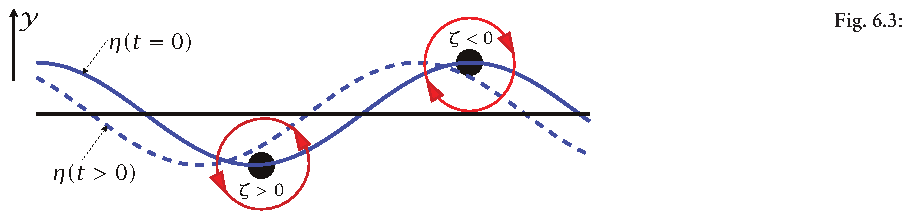
\includegraphics[width=\textwidth]{assets/fig_rossby_wave.pdf}
  \caption{
    A two-dimensional (x-y) Rossby wave.
    An initial disturbance displaces a material line at constant latitude
    (the straight horizontal line) to the solid line marked $\eta(t=0)$.
    Conservation of potential vorticity, $\zeta + \beta y$, leads to the
    production of relative vorticity, $\zeta$, as shown.
    The associated velocity field (arrows on the circles) then advects the
    fluid parcels, and the material line evolves into the dashed line with
    the phase propagating westward.
    This is Fig. 6.3 in Vallis (EAOD).
  }
  \label{fig:swe_rossby_wave}
\end{figure}

\subsection{Exercises}

\begin{enumerate}
  \item Assuming shallow water approximation and mid-latitudes, quantify the
  relative importance of planetary rotation in the flow for (a) wind-generated
  swell waves, (b) a submesoscale eddy, (c) Gulf Stream, and (d) a synoptic-scale
  cyclone in the atmosphere.
  \item Consider characteristic mid-latitude flows on Earth, Jupiter, and Titan.
  At what spatial scales does the gravity play equal role as the rotation?
  Assume the shallow water dispersion relationship for your analysis.
  \item Show that the vector identity
  \begin{equation}
    \nabla \times (\mathbf{a} \times \mathbf{b}) =
    (\mathbf{b} \cdot \nabla) \mathbf{a} - (\mathbf{a} \cdot \nabla) \mathbf{b} +
    \mathbf{a} \nabla \cdot \mathbf{b} - \mathbf{b} \nabla \cdot \mathbf{a}
  \end{equation}
  holds for arbitrary vector fields $\mathbf{a}$ and $\mathbf{b}$.
  \item An ocean eddy with initial relative vorticity $\zeta_0$ begins its
  journey northward at 30$^\circ$N and depth of 2000 m and travels with the
  mean flow to 40$^\circ$N and depth of 1000 m.
  Assuming the potential vorticity of the eddy is conserved, calculate the its
  final relative vorticity.
\end{enumerate}

\subsection*{Further reading}

\begin{itemize}
  \item Chapter 4 (Shallow water systems) of EAOD by Vallis.
  \item Section 6.3 (Rossby wave essentials) of EAOD by Vallis.
\end{itemize}

\newpage
\section{Turbulence}
\label{sec:turbulence}

Turbulence is the nonlinear and chaotic fluid motion that occurs when a fluid
is driven by sufficiently strong forces.
It is characterized by large fluctuations in time and space and over a broad
range of scales.
Fluid elements with high vorticity of either sign move and interact with each
other, transferring energy and vorticity across scales.
In this chapter, we investigate turbulence from the point of view of the
governing equations of fluid motion.
To do that, we begin by introducing the Reynolds decomposition, a fundamental
tool in the study of turbulence.
By applying it to the Navier-Stokes equation, we will derive the Reynolds-averaged
Navier-Stokes (RANS) equation, which describes and predicts the evolution of the
mean flow while accounting for the effects of turbulence.
We will discuss the so-called closure problem of turbulence, which is the
challenge of representing the effects of the smallest scales on the larger scales.
Using the RANS equation, we will derive the turbulent kinetic energy budget
equation, and investigate the turbulent cascade in both 2D and 3D flows.
The new understanding from this chapter will allow us to study the boundary
layers in the atmosphere and the ocean alike.

\subsection{Reynolds decomposition}
\label{sec:reynolds_decomposition}

We begin by introducing the decomposition of a field (in this case velocity
$\mathbf{u}$, a vector field) into the mean and fluctuating parts:

\begin{equation}
  \mathbf{u}(x, t) = \overline{\mathbf{u}}(x) + \mathbf{u}'(x, t)
\end{equation}
If we take the time average of the above equation, we get:

\begin{equation}
  \overline{\mathbf{u}(x, t)} = \overline{\overline{\mathbf{u}}(x) + \mathbf{u}'(x, t)}
\end{equation}
which leads to:

\begin{equation}
  \overline{\mathbf{u}'(x, t)} = 0
\end{equation}
The averaging operation is commutative with respect to derivatives and integrals,
over space or time alike:

\begin{equation}
  \overline{\frac{\partial \mathbf{u}}{\partial t}} = \frac{\partial \overline{\mathbf{u}}}{\partial t}
\end{equation}

\begin{equation}
  \overline{\nabla \cdot \mathbf{u}} = \nabla \cdot \overline{\mathbf{u}}
\end{equation}

\begin{equation}
  \overline{\int \mathbf{u} dt} = \int \overline{\mathbf{u}} dt
\end{equation}
Although here we have defined the Reynolds decomposition using the velocity
field, it can be applied to any field variable, vector or scalar alike.

If the flow is incompressible ($\nabla \cdot \mathbf{u} = 0$), then the mean
flow is incompressible as well:

\begin{equation}
  \nabla \cdot \overline{\mathbf{u}} = 0
\end{equation}
and by definition the fluctuating field must also be divergence-free:

\begin{equation}
  \nabla \cdot \mathbf{u} = \nabla \cdot (\overline{\mathbf{u}} + \mathbf{u}') =
  \nabla \cdot \overline{\mathbf{u}} + \nabla \cdot \mathbf{u}' = 0
\end{equation}

\begin{equation}
  \nabla \cdot \mathbf{u}' = 0
\end{equation}

We seek the governing equations for the mean flow that include the effects of
the fluctuating field (turbulence).
To do that, let's apply the Reynolds decomposition to the Navier-Stokes equation
and take the time average of the resulting equation.
We begin by writing out Eq. (\ref{eq:momentum_navier_stokes}) without the
body forces, for simplicity (as the body forces won't be affected by the
Reynolds decomposition):

\begin{equation}
  \frac{\partial \mathbf{u}}{\partial t} + (\mathbf{u} \cdot \nabla) \mathbf{u} =
  - \frac{1}{\rho} \nabla p + \nu \nabla^2 \mathbf{u}
  \label{eq:ns_reynolds1}
\end{equation}
It's at this time useful to re-cast this equation in the momentum-conservative
form that is prognostic for the momentum $\rho \mathbf{u}$ rather than just the
velocity $\mathbf{u}$.
To do that, multiply Eq. \ref{eq:ns_reynolds1} by $\rho$ to get:

\begin{equation}
  \rho \frac{\partial \mathbf{u}}{\partial t} + (\rho \mathbf{u} \cdot \nabla) \mathbf{u} =
  - \nabla p + \mu \nabla^2 \mathbf{u}
  \label{eq:ns_reynolds2}
\end{equation}
while recalling that the kinematic viscosity $\nu$ is defined as
$\nu = \mu / \rho$.
Now, we will use the Eulerian form of the continuity equation
(Eq. \ref{eq:continuity_eulerian}) to reframe the left-hand side of Eq.
\ref{eq:ns_reynolds2} in terms of the momentum $\rho \mathbf{u}$:

\begin{equation}
\begin{split}
  \rho \frac{\partial \mathbf{u}}{\partial t} + (\rho \mathbf{u} \cdot \nabla) \mathbf{u} \\
  = \frac{\partial (\rho \mathbf{u})}{\partial t} - \mathbf{u} \frac{\partial \rho}{\partial t} + (\rho \mathbf{u} \cdot \nabla) \mathbf{u} \\
  = \frac{\partial (\rho \mathbf{u})}{\partial t} + \mathbf{u} \nabla \cdot (\rho \mathbf{u}) + (\rho \mathbf{u} \cdot \nabla) \mathbf{u} \\
  = \frac{\partial (\rho \mathbf{u})}{\partial t} + \nabla \cdot (\rho \mathbf{u} \mathbf{u})
\end{split}
\end{equation}
Our momentum equation (Eq. \ref{eq:ns_reynolds2}) can then be written as:

\begin{equation}
  \frac{\partial (\rho \mathbf{u})}{\partial t} +
  \nabla \cdot (\rho \mathbf{u} \mathbf{u}) =
  - \nabla p + \mu \nabla^2 \mathbf{u}
\end{equation}
and in case of incompressible flows ($\nabla \cdot \mathbf{u} = 0$):

\begin{equation}
  \frac{\partial \mathbf{u}}{\partial t} +
  \nabla \cdot (\mathbf{u} \mathbf{u}) =
  - \frac{1}{\rho} \nabla p + \nu \nabla^2 \mathbf{u}
  \label{eq:ns_reynolds3}
\end{equation}
We are still describing the full flow with all it turbulent fluctuations.
Remember that we are interested in the solution for the mean flow that accounts
for the effects of turbulence, so we need apply the Reynolds decomposition to
$\mathbf{u}$ and $p$, time average the resulting equation, and notice that
$\overline{\mathbf{u}'}$ and $\overline{p'}$ are both zero:

\begin{equation}
  \frac{\partial \overline{\mathbf{u}}}{\partial t} +
  \nabla \cdot (\overline{\mathbf{u}} \overline{\mathbf{u}}) =
  - \frac{1}{\rho} \nabla \overline{p} + \nu \nabla^2 \overline{\mathbf{u}}
\end{equation}
Let's expand the advective term:

\begin{equation}
   \nabla \cdot (\overline{\mathbf{u} {\mathbf{u}}}) =
   \nabla \cdot [\overline{(\overline{\mathbf{u}} + \mathbf{u}')(\overline{\mathbf{u}} + \mathbf{u}')}] =
   \nabla \cdot (\overline{\overline{\mathbf{u}}\, \overline{\mathbf{u}}} + \overline{\mathbf{u}' \overline{\mathbf{u}}} + \overline{\overline{\mathbf{u}} \mathbf{u}'} + \overline{\mathbf{u}' \mathbf{u}'})
\end{equation}
which reduces to:

\begin{equation}
  \nabla \cdot (\overline{\mathbf{u} \mathbf{u}}) =
  \nabla \cdot (\overline{\mathbf{u}}\, \overline{\mathbf{u}}) + \nabla \cdot (\overline{\mathbf{u}' \mathbf{u}'})
  \label{eq:reynolds_advection_expanded}
\end{equation}
Insert Eq. (\ref{eq:reynolds_advection_expanded}) into Eq. (\ref{eq:ns_reynolds3}) to get:

\begin{equation}
  \frac{\partial \overline{\mathbf{u}}}{\partial t} +
  \nabla \cdot (\overline{\mathbf{u}}\, \overline{\mathbf{u}}) =
  - \frac{1}{\rho} \nabla \overline{p} +
  \nu \nabla^2 \overline{\mathbf{u}}
  - \nabla \cdot (\overline{\mathbf{u}' \mathbf{u}'})
  \label{eq:rans}
\end{equation}
which is the \textit{Reynolds-Averaged Navier-Stokes (RANS) equation}
\index{Reynolds!averaged Navier-Stokes equation}, the term
$\overline{\mathbf{u}' \mathbf{u}'}$ is called the \textit{Reynolds stress tensor}
\index{Reynolds!stress tensor},
and $\nabla \cdot (\overline{\mathbf{u}' \mathbf{u}'})$ is the
\textit{Reynolds stress divergence}\index{Reynolds!stress divergence}.

The Reynolds-averaged continuity equation is much simpler to derive and is
just:

\begin{equation}
  \nabla \cdot \overline{\mathbf{u}} = 0
  \label{eq:continuity_reynolds}
\end{equation}

Between Eqs. (\ref{eq:rans}) and (\ref{eq:continuity_reynolds}) we have
two equations with three unknowns: $\overline{\mathbf{u}}$, $\overline{p}$, and
$\overline{\mathbf{u}' \mathbf{u}'}$.
To close the system, we need to find an equation for the Reynolds stress tensor,
which brings us to the closure problem of turbulence.

\subsection{Closure problem}

To illustrate the closure problem of turbulence, let's try to derive the
equation for the evolution of the Reynolds stress $\overline{\mathbf{u}' \mathbf{u}'}$.
Suppose that the Reynolds stress evolves according to the yet to be determined
sources and sinks of the Reynolds stress:

\begin{equation}
  \frac{d \left( \mathbf{u}' \mathbf{u}' \right)}{dt} =
  \text{sources} - \text{sinks}
  \label{eq:reynolds_stress_evolution}
\end{equation}
Expanding the time derivative in a momentum-conservative form and time averaging
yields similar to Eq. (\ref{eq:reynolds_advection_expanded}):

\begin{equation}
  \frac{d \left( \overline{\mathbf{u}' \mathbf{u}'} \right)}{dt} =
  \frac{\partial \left( \overline{\mathbf{u}' \mathbf{u}'} \right)}{\partial t} +
  \nabla \cdot \left( \overline{\mathbf{u}} \overline{\mathbf{u}' \mathbf{u}'} \right) +
  \nabla \cdot \left( \overline{\mathbf{u}' \mathbf{u}' \mathbf{u}'} \right)
\end{equation}
See, if we try to seek the equation for the evolution of the Reynolds stress,
we end up with the flux of the flux itself as a new unknown.
Further, if we tried to seek the equation for this new cubic term, we would
end up with an equation that includes a quartic term of $\mathbf{u}'$:


\begin{equation}
  \frac{d \left( \overline{\mathbf{u}' \mathbf{u}' \mathbf{u}'} \right)}{dt} =
  \frac{\partial \left( \overline{\mathbf{u}' \mathbf{u}' \mathbf{u}'} \right)}{\partial t} +
  \nabla \cdot \left( \overline{\mathbf{u}} \overline{\mathbf{u}' \mathbf{u}' \mathbf{u}'} \right) +
  \nabla \cdot \left( \overline{\mathbf{u}' \mathbf{u}' \mathbf{u}' \mathbf{u}'} \right)
\end{equation}
The fact that we cannot close the RANS equations unless we somehow approximate
the Reynolds stress tensor is known as the closure problem of turbulence.
On one hand, it's relieving that we don't have to figure out the sources and
sinks for the Reynolds stress tensor in Eq. (\ref{eq:reynolds_stress_evolution}).
On the other hand, we still need to come up with some model or approximation
for the Reynolds stress tensor to solve the RANS equations.

\subsection{Reynolds stress}

Recall from Chapter \ref{sec:continuity_momentum} where we first derived the
Cauchy momentum equation (Eq. \ref{eq:momentum_cauchy}), ignoring the body forces
for brevity:

\begin{equation}
  \frac{\partial \mathbf{u}}{\partial t} + (\mathbf{u} \cdot \nabla) \mathbf{u} =
  \frac{1}{\rho} \nabla \cdot \boldsymbol{\sigma}
\end{equation}
and the associated stress tensor (Eq. \ref{eq:stress_tensor_decomposition}):

\begin{equation}
  \boldsymbol{\sigma} = -p \mathbf{I} + \boldsymbol{\tau}
\end{equation}
where we had described the stress tensor $\boldsymbol{\sigma}$ as a combination
of the normal stresses (pressure) on the diagonal and the deviatoric stresses
off the diagonal:

\begin{equation}
  \begin{bmatrix}
    -p + \tau_{xx} & \tau_{xy} & \tau_{xz} \\
    \tau_{yx} & -p + \tau_{yy} & \tau_{yz} \\
    \tau_{zx} & \tau_{zy} & -p + \tau_{zz}
  \end{bmatrix}
\end{equation}
Then, in Section \ref{sec:viscous_forces}, we stated that for a Newtonian fluid
the deviatoric stresses can be approximated with the velocity gradients, an
approximation that was established in the laboratory:

\begin{equation}
  \nabla \cdot \boldsymbol{\tau} = \nu \nabla^2 \mathbf{u}
\end{equation}
Now, in addition to the viscous stresses, we have the turbulent Reynolds stresses
introduced in Eq. (\ref{eq:rans}).
The turbulent Reynolds stresses arise due to the scale separation between the
large-scale mean flow and the turbulent fluctuations, which we introduced when
we applied the Reynolds decomposition to the velocity field.

Eq. (\ref{eq:rans}) can be rewritten more concisely by applying the divergence
operator to the pressure and Reynolds and viscous stresses as a whole:

\begin{equation}
  \frac{\partial \overline{\mathbf{u}}}{\partial t} +
  \nabla \cdot (\overline{\mathbf{u}}\, \overline{\mathbf{u}}) =
  \frac{1}{\rho} \nabla \cdot \left( \mu \nabla \cdot \overline{\mathbf{u}} - p - \rho \overline{\mathbf{u}' \mathbf{u}'} \right)
  \label{eq:rans_expanded}
\end{equation}
If it's not obvious already, notice that $\rho \overline{\mathbf{u}' \mathbf{u}'}$
is the only term that makes Eq. (\ref{eq:rans_expanded}) different from the
original Navier-Stokes equation (Eq. \ref{eq:ns_reynolds3}).
Thus, if we apply a scale separation (\textit{i.e.} the Reynolds decomposition)
to the velocity field such that we distinguish between the mean flow and the
fluctuations, the equation for the mean flow contains an additional term that
quantifies the contribution of the turbulent fluctuations to the mean.
Note that, strictly speaking, $\rho \overline{\mathbf{u}' \mathbf{u}'}$ is a
stress (as in, momentum flux), however it's common to refer to
$\overline{\mathbf{u}' \mathbf{u}'}$ as the Reynolds stress as well, even when
the density is omitted.

Let's look at this Reynolds stress tensor in more detail.
Using our usual notation for the velocity vector to be $\mathbf{u} = (u, v, w)$,
the components of the Reynolds stress tensor are:

\begin{equation}
  \overline{u'u'} = \begin{bmatrix}
    \overline{u'u'} & \overline{u'v'} & \overline{u'w'} \\
    \overline{v'u'} & \overline{v'v'} & \overline{v'w'} \\
    \overline{w'u'} & \overline{w'v'} & \overline{w'w'}
  \end{bmatrix}
\end{equation}
The diagonal components of this tensor ($\overline{u'u'}$, $\overline{v'v'}$, and
$\overline{w'w'}$) are called the \textit{normal stresses}, and the off-diagonal
components ($\overline{u'v'}$, $\overline{u'w'}$, $\overline{v'w'}$) are called
the \textit{shear stresses}.
The Reynolds stress tensor is symmetric, which means that
$\overline{u'v'} = \overline{v'u'}$, $\overline{u'w'} = \overline{w'u'}$, and
$\overline{v'w'} = \overline{w'v'}$.
It is only the shear stresses that contribute to the turbulent transport of
momentum.
An important property of boundary layer physics, the
\textit{Turbulent Kinetic Energy}\index{Turbulent!Kinetic energy} (TKE) is half
the sum of the diagonal components of the Reynolds stress tensor:

\begin{equation}
  k = \frac{1}{2} \left( \overline{u'u'} + \overline{v'v'} + \overline{w'w'} \right)
\end{equation}
From the point of view of the Reynolds decomposition into the mean and
fluctuations from the mean, TKE is the sum of velocity variances.
TKE plays an important role in parameterizing the subgrid-scale turbulent
processes in the boundary layer components of weather and ocean prediction
models.
$\overline{u'w'}$ and $\overline{v'w'}$ are also very important quantities in
the study of air-sea interaction, as they govern the momentum exchange between
the atmospheric surface layer, the ocean surface waves, and the upper-ocean
boundary layer.

In numerical models, the vector equations must be written out explicitly in
scalar component form.
It's thus a useful exercise to write out the RANS equation
(Eq. \ref{eq:rans_expanded}) as a system of scalar equations, one for each
component of the mean velocity vector:

\begin{equation}
  \frac{\partial \overline{u}}{\partial t} + 
  \frac{\partial \overline{u} \overline{u}}{\partial x} +
  \frac{\partial \overline{v} \overline{u}}{\partial y} +
  \frac{\partial \overline{w} \overline{u}}{\partial z} =
  - \frac{1}{\rho} \frac{\partial \overline{p}}{\partial x}
  - \frac{\partial \overline{u'u'}}{\partial x} - \frac{\partial \overline{v'u'}}{\partial y} - \frac{\partial \overline{w'u'}}{\partial z}
  + \nu \left( \frac{\partial^2 \overline{u}}{\partial x^2} + 
               \frac{\partial^2 \overline{u}}{\partial y^2} +
               \frac{\partial^2 \overline{u}}{\partial z^2}
        \right)
\end{equation}

\begin{equation}
  \frac{\partial \overline{v}}{\partial t} + 
  \frac{\partial \overline{u} \overline{v}}{\partial x} +
  \frac{\partial \overline{v} \overline{v}}{\partial y} +
  \frac{\partial \overline{w} \overline{v}}{\partial z} =
  - \frac{1}{\rho} \frac{\partial \overline{p}}{\partial y}
  - \frac{\partial \overline{u'v'}}{\partial x} - \frac{\partial \overline{v'v'}}{\partial y} - \frac{\partial \overline{w'v'}}{\partial z}
  + \nu \left( \frac{\partial^2 \overline{v}}{\partial x^2} + 
               \frac{\partial^2 \overline{v}}{\partial y^2} +
               \frac{\partial^2 \overline{v}}{\partial z^2}
        \right)
\end{equation}

\begin{equation}
  \frac{\partial \overline{w}}{\partial t} + 
  \frac{\partial \overline{u} \overline{w}}{\partial x} +
  \frac{\partial \overline{v} \overline{w}}{\partial y} +
  \frac{\partial \overline{w} \overline{w}}{\partial z} =
  - \frac{1}{\rho} \frac{\partial \overline{p}}{\partial z}
  - \frac{\partial \overline{u'w'}}{\partial x} - \frac{\partial \overline{v'w'}}{\partial y} - \frac{\partial \overline{w'w'}}{\partial z}
  + \nu \left( \frac{\partial^2 \overline{w}}{\partial x^2} + 
               \frac{\partial^2 \overline{w}}{\partial y^2} +
               \frac{\partial^2 \overline{w}}{\partial z^2}
        \right)
\end{equation}

\subsection{Turbulent kinetic energy budget}

Turbulent kinetic energy (TKE) is a fundamental quantity in the study of
turbulence.
It's a prognostic variable in many subgrid-scale parametric models of
atmospheric and oceanic boundary layers.
Here we derive the prognostic equation for TKE from the fundamental equations
with Reynolds decomposition, often referred to as the TKE budget equation.

The derivation of the TKE budget equation involves the following steps:

\begin{enumerate}
  \item Start from the Navier-Stokes equation (Eq. \ref{eq:ns_reynolds1})
  and apply the Reynolds decomposition to the velocity field.
  \item Subtract the RANS equation from the original Navier-Stokes equation
  with Reynolds decomposition to obtain the equation for the velocity
  fluctuations.
  \item Multiply the equation for the velocity fluctuations by the fluctuating
  velocity components and time-average to obtain the equation for the TKE.
\end{enumerate}

For completeness, we will also consider the buoyancy term that we derived in
the Boussinesq approximation, as it will turn out that this term plays a role
in the TKE budget.
We start from the Navier-Stokes equation but in the advective (non-conservative)
form, rather than the flux (conservative) form, as the advective form makes the
TKE budget derivation more straightforward (they are equivalent for
incompressible flows, $\nabla \cdot \mathbf{u} = 0$).

\begin{equation}
  \frac{\partial \mathbf{u}}{\partial t} + 
  (\mathbf{u} \cdot \nabla) \mathbf{u} =
  - \frac{1}{\rho} \nabla p
  + \frac{\delta \rho}{\rho} \mathbf{g}
  + \nu \nabla^2 \mathbf{u}
\end{equation}
Apply the Reynolds decomposition to $\mathbf{u}$, $p$, and $\delta \rho$ to get:

\begin{equation}
  \begin{split}
  \frac{\partial \overline{\mathbf{u}}}{\partial t} + \frac{\partial \mathbf{u}'}{\partial t} +
  (\overline{\mathbf{u}} \cdot \nabla) \overline{\mathbf{u}} +
  (\mathbf{u}' \cdot \nabla) \overline{\mathbf{u}} +
  (\overline{\mathbf{u}} \cdot \nabla) \mathbf{u}' +
  (\mathbf{u}' \cdot \nabla) \mathbf{u}' = \\
  - \frac{1}{\rho} \nabla \overline{p}
  - \frac{1}{\rho} \nabla p'
  + \frac{\overline{\delta \rho}}{\rho} \mathbf{g}
  + \frac{\delta \rho'}{\rho} \mathbf{g}'
  + \nu \nabla^2 \overline{\mathbf{u}}
  + \nu \nabla^2 \mathbf{u}'
  \end{split}
  \label{eq:tke_budget_ns}
\end{equation}
The RANS equation in the advective form is:

\begin{equation}
  \frac{\partial \overline{\mathbf{u}}}{\partial t} +
  (\overline{\mathbf{u}} \cdot \nabla) \overline{\mathbf{u}} +
  \overline{(\mathbf{u}' \cdot \nabla) \mathbf{u}'} = \\
  - \frac{1}{\rho} \nabla \overline{p}
  + \frac{\overline{\delta \rho}}{\rho} \mathbf{g}
  + \nu \nabla^2 \overline{\mathbf{u}}
  \label{eq:tke_budget_rans}
\end{equation}
Subtract Eq. (\ref{eq:tke_budget_rans}) from Eq. (\ref{eq:tke_budget_ns}) to
obtain the equation for the velocity fluctuations:

\begin{equation}
  \frac{\partial \mathbf{u}'}{\partial t} +
  (\mathbf{u}' \cdot \nabla) \overline{\mathbf{u}} +
  (\overline{\mathbf{u}} \cdot \nabla) \mathbf{u}' +
  (\mathbf{u}' \cdot \nabla) \mathbf{u}' -
  \overline{(\mathbf{u}' \cdot \nabla) \mathbf{u}'} = \\
  - \frac{1}{\rho} \nabla p'
  + \frac{\delta \rho'}{\rho} \mathbf{g}
  + \nu \nabla^2 \mathbf{u}'
\end{equation}
Multiply by $\mathbf{u}'$ to get:

\begin{equation}
  \mathbf{u}'\frac{\partial \mathbf{u}'}{\partial t} +
  \mathbf{u}' (\mathbf{u}' \cdot \nabla) \overline{\mathbf{u}} +
  \mathbf{u}' (\overline{\mathbf{u}} \cdot \nabla) \mathbf{u}' +
  \mathbf{u}' (\mathbf{u}' \cdot \nabla) \mathbf{u}' -
  \mathbf{u}' \overline{(\mathbf{u}' \cdot \nabla) \mathbf{u}'} = \\
  - \frac{1}{\rho} \mathbf{u}' \nabla p'
  + \frac{\delta \rho'}{\rho} \mathbf{u}' \mathbf{g}
  + \nu \mathbf{u}' \nabla^2 \mathbf{u}'
\end{equation}
Rearrange the terms:

\begin{equation}
  \begin{split}
  \frac{\partial}{\partial t} \left( \frac{\mathbf{u}'^2}{2} \right) +
  (\overline{\mathbf{u}} \cdot \nabla) \left( \frac{\mathbf{u}'^2}{2} \right) +
  (\mathbf{u}' \mathbf{u}' \cdot \nabla) \overline{\mathbf{u}} +
  \frac{1}{2} \nabla \cdot (\mathbf{u}' \mathbf{u}' \mathbf{u}') -
  \mathbf{u}' \overline{(\mathbf{u}' \cdot \nabla) \mathbf{u}'} = \\
  - \frac{1}{\rho} \mathbf{u}' \nabla p'
  + \frac{\delta \rho'}{\rho} \mathbf{u}' \cdot \mathbf{g}
  + \nu \mathbf{u}' \nabla^2 \mathbf{u}'
  \end{split}
\end{equation}
Finally, time-average to get the TKE budget equation, noting that the last term
on the left-hand side drops out due to time-averaging, and that
$k \equiv \frac{1}{2} \overline{\mathbf{u}'^2}$:

\begin{equation}
  \frac{\partial k}{\partial t} + \overline{\mathbf{u}} \cdot \nabla k =
  - \frac{1}{2} \nabla \cdot (\overline{\mathbf{u}' \mathbf{u}' \mathbf{u}'})
  - (\mathbf{u}' \mathbf{u}' \cdot \nabla) \overline{\mathbf{u}}
  - \frac{1}{\rho} \overline{\mathbf{u}' \nabla p'}
  + \overline{\frac{\delta \rho'}{\rho} \mathbf{u}' \cdot \mathbf{g}}
  + \nu \overline{\mathbf{u}' \nabla^2 \mathbf{u}'}
  \label{eq:tke_budget_near_final}
\end{equation}
So far we broke down the advective term from the original Navier-Stokes equation
to produce three new terms.
We're still left with the viscous term, which can be rearranged into two terms
for a more intuitive physical interpretation.
Here we'll use the following identity to expand the Laplacian:

\begin{equation}
  \overline{\nu \mathbf{u}' \nabla^2 \mathbf{u}'} =
  \nu \nabla \cdot (\overline{\mathbf{u}' \nabla \mathbf{u}'}) -
  \nu \overline{\nabla \mathbf{u}' \cdot \nabla \mathbf{u}'} =
  \nu \nabla^2 k - \nu \overline{(\nabla \mathbf{u}' \cdot \nabla \mathbf{u}')}
  \label{eq:tke_budget_viscous}
\end{equation}
Inserting Eq. (\ref{eq:tke_budget_viscous}) into Eq. (\ref{eq:tke_budget_near_final})
gives us our final form of the TKE budget equation:

\begin{equation}
  \frac{\partial k}{\partial t} + \overline{\mathbf{u}} \cdot \nabla k =
  - \frac{1}{2} \nabla \cdot (\overline{\mathbf{u}' \mathbf{u}' \mathbf{u}'})
  - (\overline{\mathbf{u}' \mathbf{u}'} \cdot \nabla) \overline{\mathbf{u}}
  - \frac{1}{\rho} \overline{\mathbf{u}' \nabla p'}
  + \overline{\frac{\delta \rho'}{\rho} \mathbf{u}' \cdot \mathbf{g}}
  + \nu \nabla^2 k
  - \nu \overline{\nabla \mathbf{u}' \cdot \nabla \mathbf{u}'}
  \label{eq:tke_budget_final}
\end{equation}
Let's look at each term in Eq. (\ref{eq:tke_budget_final}) and discuss its
physical meaning:

\begin{itemize}
  \item $\frac{\partial k}{\partial t}$: Eulerian rate of change of TKE in
  a fixed point in space.

  \item $\overline{\mathbf{u}} \cdot \nabla k$: Advection of TKE by the mean
  flow. Like any other fluid property, TKE as well is subject to advection by
  the mean flow, \textit{i.e.} $dk/dt = \partial k/\partial t + \overline{\mathbf{u}} \cdot \nabla k$.

  \item $-\frac{1}{2} \nabla \cdot (\overline{\mathbf{u}' \mathbf{u}' \mathbf{u}'})$
  is the turbulent transport of TKE. In other words, this term quantifies how
  much turbulent eddies are transported by the turbulent eddies themselves.

  \item $-(\overline{\mathbf{u}' \mathbf{u}'} \cdot \nabla) \overline{\mathbf{u}}$ is the
  production of TKE by the mean flow, also known as the shear production.

  \item $-\frac{1}{\rho} \overline{\mathbf{u}' \nabla p'}$ is the
  production of TKE by the turbulent fluctuations of the pressure gradient,
  also known as pressure diffusion.

  \item $\overline{\frac{\delta \rho'}{\rho} \mathbf{u}' \cdot \mathbf{g}}$
  is the production of TKE by buoyancy. Notice the dot product between the
  velocity vector and the gravitational acceleration, which means that the
  buoyancy production occurs only by the vertical velocity component, and is
  scaled by the buoyancy anomaly $\delta \rho'$. The stronger the stratification
  of the fluid, the larger the buoyancy production (or dissipation, depending on
  the sign of stratification) of TKE.

  \item $\nu \nabla^2 k$ is the dissipation of TKE by molecular diffusion.

  \item $-\nu \overline{\nabla \mathbf{u}' \cdot \nabla \mathbf{u}'}$ is the 
  turbulent eddy dissipation of TKE. Note that $\nabla \mathbf{u}'$ are rank-2
  tensors, so the inner product $\nabla \mathbf{u}' \cdot \nabla \mathbf{u}'$
  is a rank-4 tensor, which is averaged to get a scalar.
\end{itemize}

Given Eq. (\ref{eq:tke_budget_final}) and the interpretation of its terms,
we can proceed to apply dimensional analysis in an attempt to learn the
distribution and transfer of turbulence across spatial scales.

\subsection{Turbulent cascade}

The two most common sources of turbulence are shear (mechanical) and buoyancy
(thermodynamic).
As such, the turbulent energy is predominantly generated at the larger scales,
where the largest coherent eddies tend to be of the same scale as the flow
itself.
For example, the largest eddies that the Gulf Stream sheds are of similar
diameter as the width of the Gulf Stream itself.
Similarly, the largest eddies in a coffee cup are of similar size as the spoon
that does the stirring.
An example of buoyancy generation of turbulence is the convection in the 
atmospheric boundary layer due to cool air over warm land or ocean surface.
So, most turbulence tends to be produced at the scales many orders of magnitude
that of the viscous scales.
At the smallest scales, we know that viscosity does the work to dissipate
mechanical energy into heat.
What happens between the largest and the smallest scales is less clear and is
the subject of this section.
A concept of \textit{turbulent energy cascade}\index{Turbulent!Energy cascade},
first introduced by Richardson (1922)\index{Richardson},
suggests that the energy is transferred from the large to the small scales,
and that this transfer is a cascade.
He put it succinctly as:

\begin{quote}
  \textit{
    \noindent Big whirls have little whirls,\\
    Which feed on their velocity;\\
    And little whirls have lesser whirls,\\
    And so on to viscosity.
  }
\end{quote}

To answer how the velocity statistics are distributed from the largest to the
smallest scales, we evaluate the TKE budget equation for a very turbulent flow
in which $Re = UL/\nu$ is very large.
The turbulent cascade is illustrated in Fig. \ref{fig:turbulent_cascade}.

\begin{figure}[h]
  \centering
  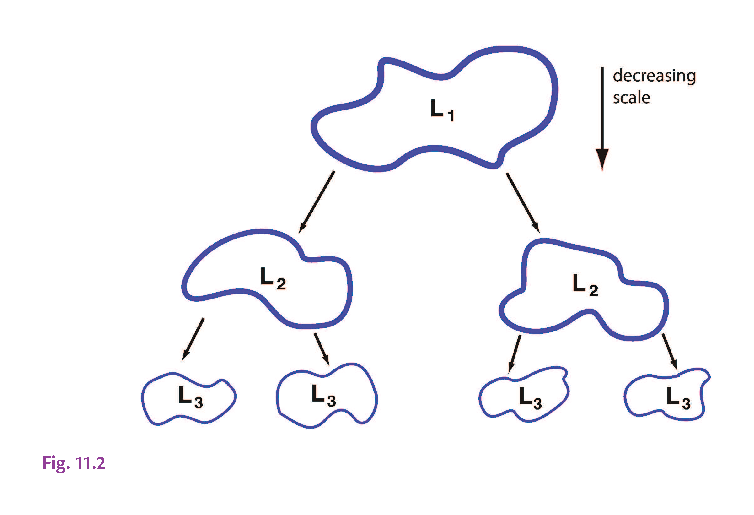
\includegraphics[width=0.8\textwidth]{assets/fig_turbulent_energy_cascade.pdf}
  \caption{
    The passage of energy to smaller scales: eddies at large scale break up
    into ones at smaller scale, thereby transferring energy to smaller scales.
    The eddies in reality are embedded within each other.
    If the passage occurs between eddies of similar sizes (\textit{i.e.}, if
    it is spectrally local), the transfer is said to be a cascade.
    This is Figure 11.2 from Vallis (AOFD).
  }
  \label{fig:turbulent_cascade}
\end{figure}

We may first ask at what length scale does the viscosity become a dominant
player.
As useful tools we will recall dimensional analysis and the Reynolds number,
which quantified the relative importance of inertial over viscous forces.

\begin{equation}
  Re = \frac{UL}{\nu}
\end{equation}
If we know that at the largest (think, geophysical) scales the viscosity is
negligible (large $Re$), we could say that the viscosity becomes more important
than turbulent motion at the scale at which $Re \approx 1$.
From there, we can define the viscous length scale as:

\begin{equation}
  L_\nu = \frac{\nu}{U}
  \label{eq:viscous_length_scale}
\end{equation}
What are some characteristic values of $L_\nu$ in the ocean and in the atmosphere?
An ocean flow with $U \approx 10^{-1}$ m/s and viscosity of $\nu \approx 10^{-6}$ m$^2$/s
gives $L_\nu \approx 10^{-5}$ m, or, one hundredth of a millimeter.
In the atmosphere with $U \approx 10$ m/s and viscosity of $\nu \approx 10^{-5}$ m$^2$/s,
we get $L_\nu \approx 10^{-6}$ m, or, one micron.
These are obviously very small scales.

To answer what happens to the flow statistics between the largest scales at
which the turbulence is generated and the smalles scales at which viscosity
dissipates all mechanical energy into heat, Kolmogorov (1941) proposed a new
Kolmogorov's three turbulence hypotheses are: 

\begin{enumerate}
  \item \textbf{Hypothesis of local isotropy:} At sufficiently high $Re$ and
  sufficiently small $L$, the turbulence is \textit{locally isotropic},
  \textit{i.e.} the flow statistics at a point are the same in all directions.
  \item \textbf{First similarity hypothesis:} At sufficiently high $Re$ and
  sufficiently small $L$, the flow statistics have a universal form
  that is uniquely determined by the viscosity $\nu$ and the energy dissipation 
  rate $\varepsilon$.
  \item \textbf{Second similarity hypothesis:} At sufficiently high $Re$ and
  and sufficiently large $L$, the flow statistics have a universal form
  that is uniquely determined by the energy dissipation rate $\varepsilon$,
  and that is independent of viscosity $\nu$.
\end{enumerate}
The energy dissipation rate $\varepsilon$ comes straight from the TKE budget
equation (Eq. \ref{eq:tke_budget_final}) and is defined as:

\begin{equation}
  \varepsilon = \nu \overline{\nabla \mathbf{u}' \cdot \nabla \mathbf{u}'}
\end{equation}

In a nutshell, Kolmogorov's three hypotheses state that a turbulent flow at
sufficiently small scales is the same looking in all directions, that
statistically all such turbulent flows are the same, and that they are uniquely
determined by either by energy dissipation rate alone, or by the energy
dissipation rate and viscosity, depending on the scale.
Through dimensional analysis, Kolmogorov also introduced the fundamental
turbulent scales, now commonly known as Kolmogorov scales:

\begin{itemize}
  \item $\eta \equiv \left( \nu^3/\varepsilon \right)^{1/4}$, or,
  Kolmogorov length scale, is the scale at which the energy dissipation by
  molecular diffusion balances the energy input by the mean flow.
  \item $u_\eta \equiv \left( \varepsilon \nu \right)^{1/4}$ is
  the velocity at the Kolmogorov length scale.
  \item $\tau_\eta \equiv \left( \nu/\varepsilon \right)^{1/2}$ is the
  Kolmogorov time scale at which the smallest coherent eddy can exist.
\end{itemize}
Any flow feature at scales smaller than these is governed by viscous dissipation
of kinetic energy into heat.

Examining the Reynolds number using the Kolmogorov scales indeed shows that
it reduces to unity, consistent with Eq. (\ref{eq:viscous_length_scale}):

\begin{equation}
  Re_\eta = \frac{u_\eta \eta}{\nu} = \frac{\left( \varepsilon \nu \right)^{1/4} \left( \nu^3/\varepsilon \right)^{1/4}}{\nu} = 1
\end{equation}

\begin{figure}[h]
  \centering
  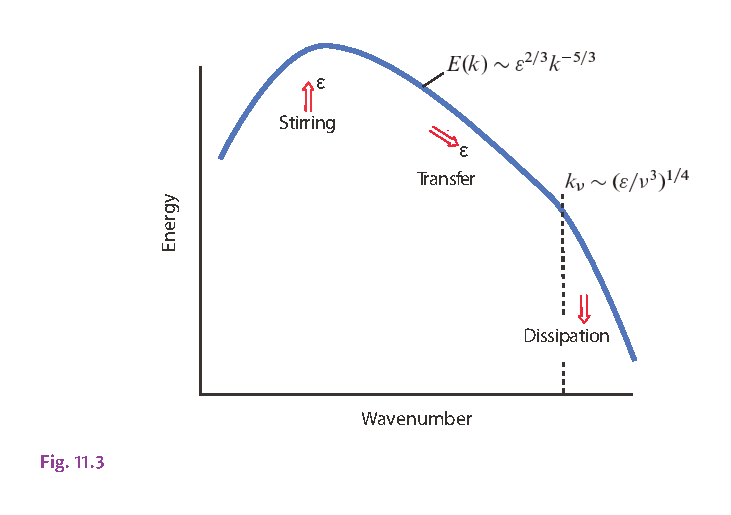
\includegraphics[width=0.8\textwidth]{assets/fig_turbulent_spectrum_3d.pdf}
  \caption{
    The energy spectrum in three-dimensional turbulence, in the theory of
    Kolmogorov (1941). Energy is supplied at some rate $\varepsilon$;
    it is cascaded to small scales, where it is ultimately dissipated by
    viscosity.
    There is no systematic energy transfer to scales larger than the forcing
    scale, so here the energy falls off.
    This is Figure 11.3 from Vallis (AOFD).
  }
  \label{fig:turbulent_spectrum_3d}
\end{figure}

Now, we may ask, how is the turbulent energy distributed across the scales?
Define the energy spectrum $E(k)$ as the energy per unit mass per unit wavenumber:

\begin{equation}
  E = \frac{1}{2} \int \mathbf{u}'^2(k)\ dk = \int E(k)\ dk
\end{equation}

What is the form of the energy spectrum $E(k)$?
Kolmogorov's second similarity hypothesis states that the energy spectrum is
universal and uniquely determined by the energy dissipation rate $\varepsilon$.
If that is true, then it must be some function of $\varepsilon$ and $k$:

\begin{equation}
  E(k) = F(\varepsilon, k)
\end{equation}
The dimensions of $E(k)$ are $L^3 T^{-2}$.
Since the wavenumber $k$ has dimensions of $L^{-1}$ and thus no temporal
dependence, the only way it can match the dimensions of $E(k)$ is if the
energy spectrum scales with $\varepsilon^{2/3}$:

\begin{equation}
  E(k) = \varepsilon^{2/3} G(k)
\end{equation}

\begin{equation}
  \frac{L^3}{T^2} \sim \frac{L^{4/3}}{T^2} G(k)
\end{equation}
where $G(k)$ is some yet to be determined function of $k$.
Then, by dimensional analysis, $g(k)$ must have dimensions of $L^{5/3}$,
making the energy spectrum:

\begin{equation}
  E(k) = \mathcal{K} \varepsilon^{2/3} k^{-5/3}
\end{equation}
where $\mathcal{K}$ is a constant not determined by Kolmogorov's theory.
The functional form of $E(k)$ is known as the Kolmogorov 5/3 law and is
illustrated in Figure \ref{fig:turbulent_spectrum_3d}.

\newpage
\section{Boundary layers}

Boundary layers occur when a fluid flows over some kind of boundary, whether
rigid or free, stationary or moving.
They are both interesting and convenient because they constrain the flow near
the boundary and thus allow simplifications that may lead to analytical solutions.
They are important because they are often the dominant flow structure in geophysical
flows.
For example, a planetary boundary layer separates the atmosphere from the surface
of the Earth.
The surface beneath the planetary boundary layer may be rigid (land or sea ice)
or free (ocean), and its roughness and thermodynamic properties may vary greatly
from place to place.
In this chapter, we start from the simplest boundary layer, a channel flow, and
derive the stress and mean velocity profiles in laminar flows.
Then, we zoom into the vertical structure of the boundary layer in turbulent
flows, and examine different regimes that occur depending on the distance from
the boundary.

\subsection{Channel flow}

A channel flow is a classic problem in fluid mechanics that is both relevant to
engineering applications, and analogous to larger-scale geophysical flows.
We begin by setting up the problem and establishing the governing equations
and the notation that we will use.
Then, we explore some analytical and numerical solutions for the time-mean
flow structure within the channel.

\subsubsection{Governing equations and boundary conditions}

\begin{figure}[h]
  \centering
  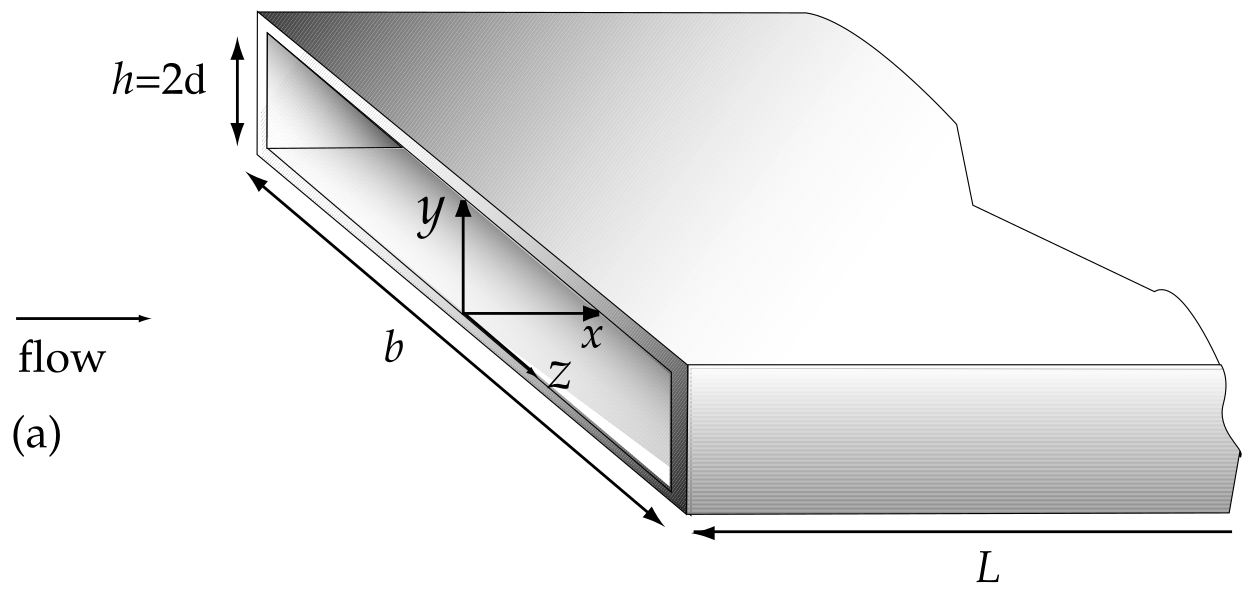
\includegraphics[width=0.8\textwidth]{assets/fig_channel_flow.png}
  \caption{
    Sketch of a channel flow.
    The height of the channel is $h$ and the flow is in the $x$ direction.
    Although the vertical and the cross-stream coordinates are denoted as $y$
    and $z$ here, respectively, we will be using the opposite notation with $z$
    being the vertical coordinate and $y$ the cross-stream coordinate.
    This is Figure 7.1a from Turbulent Flows by Pope.
  }
  \label{fig:channel_flow}
\end{figure}

Let's examine a flow in a channel between two flat plates, spaced apart by a
a distance $h = 2\delta$, such that $\delta$ represents the centerline distance
between the plates (Fig. \ref{fig:channel_flow}).
The channel is long ($L \gg \delta$) and wide ($W \gg \delta$), so there is no
variability in the $x$ and $y$ directions.
The mean flow is predominantly in the $x$ direction, so if the velocity is
defined as having components $u$, $v$, and $w$ in the streamwise, spanwise,
and vertical directions, respectively, then:

\begin{equation}
  \overline{u}(z) > 0
\end{equation}

\begin{equation}
  \overline{v} = 0
\end{equation}

For simplicity, we won't consider what happens at the very entrance into the
channel where the flow develops, and we'll only consider the fully developed
flow well into the channel such that $\partial \overline{u}/\partial x = 0$.
Thus, from a statistical point of view, this is a stationary, one-dimensional
flow that varies only in the $z$ direction.

The flow can be characterized using two different Reynolds numbers:

\begin{equation}
  Re \equiv \frac{\left<\overline{u}\right> 2 \delta}{\nu}
  \label{eq:Re_bulk}
\end{equation}
where $\left<\overline{u}\right>$ is the mean velocity in the channel (often also called
\textit{bulk velocity}):

\begin{equation}
  \left< \overline{u}\right> = \frac{1}{\delta} \int_0^{\delta} \overline{u}(z)\ dz
  \label{eq:bulk_velocity}
\end{equation}
Another useful Reynolds number is the one based on the centerline distance
between the plates:

\begin{equation}
  Re_0 \equiv \frac{u_0 \delta}{\nu}
\end{equation}
where $u_0$ is the centerline velocity $u(z=\delta)$.
Based on laboratory experiments, we know that the channel flow is laminar
for $Re < 1350$ and turbulent for $Re > 1800$, with transitional effects
observable up to $Re \approx 3000$.

Start from the Reynolds-averaged Navier-Stokes equation for $\overline{u}$:

\begin{equation}
  \frac{\partial \overline{u}}{\partial t} + 
  \overline{u} \frac{\partial \overline{u}}{\partial x} + 
  \overline{v} \frac{\partial \overline{u}}{\partial y} + 
  \overline{w} \frac{\partial \overline{u}}{\partial z} =
  - \frac{1}{\rho} \frac{\partial \overline{p}}{\partial x} +
  \nu \left( \frac{\partial^2 \overline{u}}{\partial x^2} +
  \frac{\partial^2 \overline{u}}{\partial y^2} +
  \frac{\partial^2 \overline{u}}{\partial z^2} \right)
  - \frac{\partial}{\partial x}\overline{u'u'}
  - \frac{\partial}{\partial y}\overline{u'v'}
  - \frac{\partial}{\partial z}\overline{u'w'}
  \label{eq:channel_ns_u1}
\end{equation}

For an incompressible flow, the continuity is $\nabla \cdot \overline{\mathbf{u}} = 0$,
which is effectively $\partial \overline{w}/\partial z = 0$ since the flow
doesn't vary in the $x$ and $y$ directions.
$\overline{w}$ must be zero as we can't have any flow through the walls of the channel,
and so continuity requires that $\overline{w}$ is zero everywhere.
Accounting for stationarity ($\partial \overline{u}/\partial t = 0$),
homogeneity in the $x$ and $y$ directions
($\partial \overline{u}/\partial x = \partial \overline{u}/\partial y = 0$),
and the fact that $\overline{w} = 0$, Eq. (\ref{eq:channel_ns_u1}) greatly
simplifies to:

\begin{equation}
  \frac{\partial \overline{p}}{\partial x} =
  \rho \nu \frac{\partial^2 \overline{u}}{\partial z^2} -
  \rho \frac{\partial}{\partial z}\overline{u'w'}
\end{equation}
This stationary, one-dimensional flow is thus driven by the streamwise pressure
gradient that is balanced by the normal viscous stress and the cross-stream
Reynolds stress.
The above can be further simplified to:

\begin{equation}
  \frac{\partial \overline{p}}{\partial x} =
  \frac{\partial \tau}{\partial z}
\end{equation}
where stress $\tau$ is the sum of the viscous and the turbulent Reynolds
stresses:

\begin{equation}
  \tau = \rho \left( \nu \frac{\partial \overline{u}}{\partial z} - \overline{u'w'} \right)
  \label{eq:channel_tau}
\end{equation}

Since the flow is stationary, the streamwise pressure gradient that drives it
must be constant, and so does the vertical stress gradient as well:

\begin{equation}
  \frac{\partial \tau}{\partial z} = \text{constant}
\end{equation}
Assuming symmetry around the centerline of the channel requires that the stress
there is zero (as there should not be any mean transport through the centerline).
Integrating the above from $z=0$ to $z=\delta$ we get:

\begin{equation}
  \tau(z) = a z + b
\end{equation}
where $a$ and $b$ are constants.
Use the boundary conditions $\tau(z=0) = \tau_w$ and $\tau(z=\delta) = 0$ to get:

\begin{equation}
  \tau(z) = \tau_w \left( 1 - \frac{z}{\delta} \right)
  \label{eq:channel_tau_profile}
\end{equation}
where $\tau_w$ is the so-called wall stress whose value is yet to be determined.
The stress thus decreases linearly from $\tau_w$ at the bottom wall to zero at
the centerline, reaching $-\tau_w$ at the top wall.

\subsection{Laminar flow}

What does the velocity profile look like in the case of laminar flow?
We can drop the Reynolds stress term in Eq. (\ref{eq:channel_tau}) and combine
it with Eq. (\ref{eq:channel_tau_profile}) to get:

\begin{equation}
  \frac{\partial \overline{u}}{\partial z} = \frac{\tau_w}{\rho \nu} \left(1 - \frac{z}{\delta}\right)
\end{equation}
Integrate the above with respect to $z$ to get:

\begin{equation}
  \overline{u}(z) = \frac{\tau_w z}{\rho \nu} \left(1 - \frac{z}{2\delta} \right)
\end{equation}
The velocity profile thus has a quadratic form that reaches zero at either wall,
and that has a centerline value of:

\begin{equation}
  u_0 = \overline{u}(z=\delta) = \frac{\tau_w \delta}{2 \rho \nu}
\end{equation}

The preceding equations determine the stress and velocity profiles strictly in
laminar flows, \textit{i.e.} for relatively small Reynolds numbers.
Let's see what the profiles may look like in turbulent flows.

\subsection{Turbulent flow}

\begin{figure}[h]
  \centering
  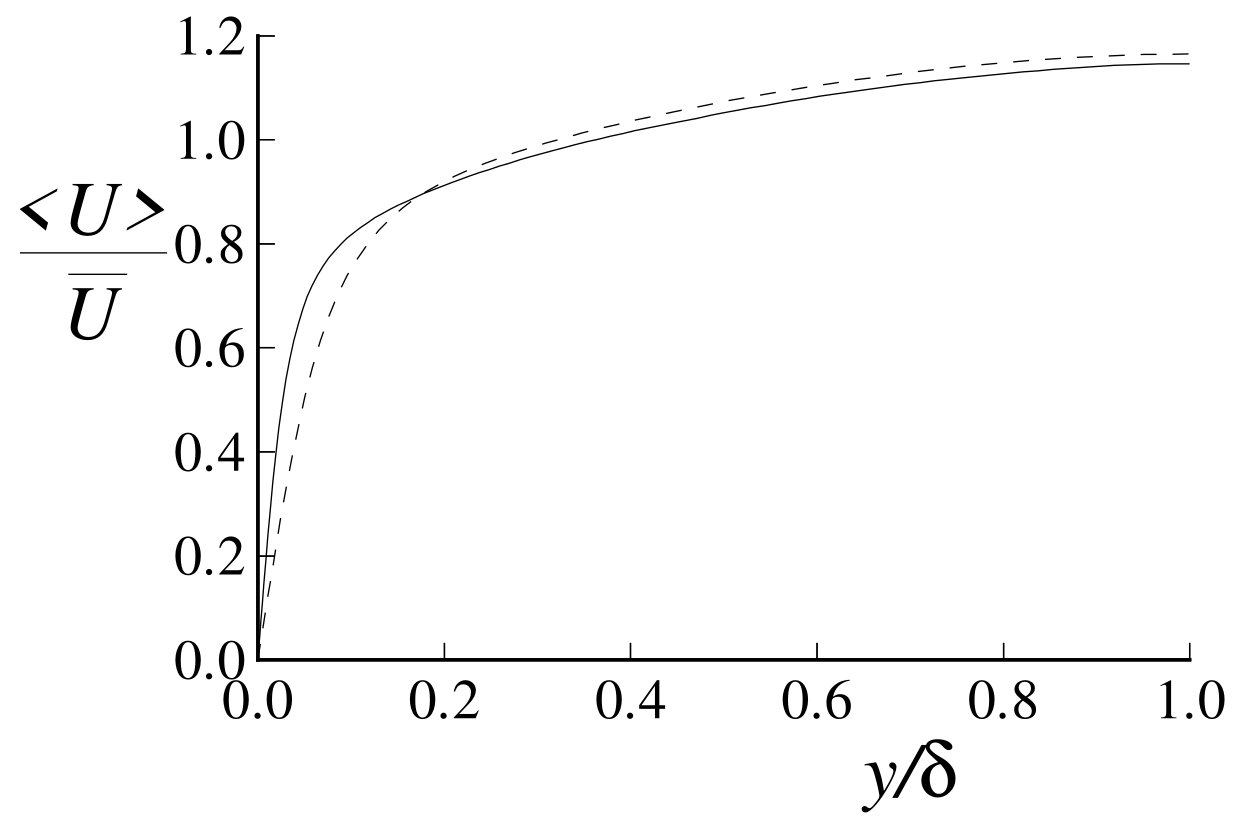
\includegraphics[width=0.6\textwidth]{assets/fig_channel_flow_turbulent_u.png}
  \caption{
    Mean velocity profile normalized by the bulk velocity in a fully developed
    turbulent channel flow, from the DNS of Kim et al. (1987).
    Dashed and solid lines are for $Re = 5,600$ and $Re = 13,750$, respectively.
    Note that in the axis labels, $y$ is the vertical coordinate and the
    angle brackets and overline denote averaging in the opposite sense from
    our notation in the main text.
    This is Figure 7.2 from Turbulent Flows by Pope.
  }
  \label{fig:channel_flow_turbulent_u}
\end{figure}

\begin{figure}[h]
  \centering
  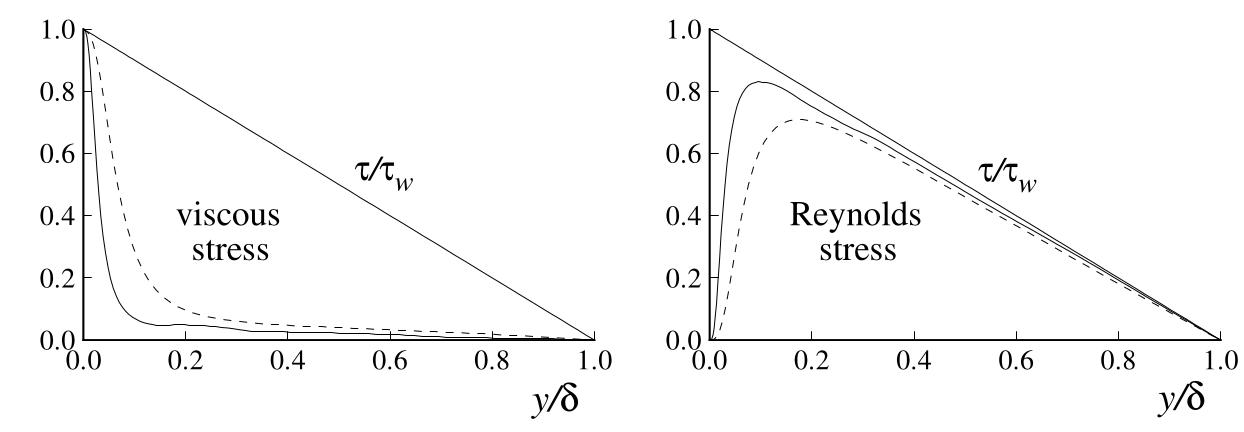
\includegraphics[width=\textwidth]{assets/fig_channel_flow_stress_profiles.png}
  \caption{
    As in Fig. \ref{fig:channel_flow_turbulent_u}, but for the vertical profiles
    of the viscous and turbulent Reynolds stresses.
    This is Figure 7.3 from Turbulent Flows by Pope.
  }
  \label{fig:channel_flow_stress_profiles}
\end{figure}
In the laminar case, we were able to analytically derive the velocity and stress
profiles.
However, in the turbulent case, the problem is much more complex and analytical
solutions are not feasible due to the presence of the turbulent Reynolds stress
term.
Direct Numerical Simulations (DNS) reveal what a turbulent velocity profile
in a channel may look like (Fig. \ref{fig:channel_flow_turbulent_u}).

At the boundaries, we can't have any flow through the walls of the channel,
the velocity and thus the turbulent Reynolds stresses must be zero, and so the
wall shear stress must be entirely due to the viscosity:

\begin{equation}
  \tau_w = \rho \nu \left( \frac{\partial \overline{u}}{\partial z} \right)_{z=0}
  \label{eq:wall_stress}
\end{equation}
Recall from Eq. (\ref{eq:channel_tau}) that the stress $\tau$ is always composed
of the viscous and turbulent parts.
However, in turbulent flows, the relative contributions of the viscous and
turbulent parts vary greatly as we move away from the wall.
Fig. \ref{fig:channel_flow_turbulent_u} shows how, in a well developed turbulent
flow, the mean velocity increases as we move further away from the wall.
At about 0.4 of the way toward the centerline, the time-mean velocity
approximately equals the bulk velocity, and exceeds it as we approach the
centerline.
The profiles are also somewhat different depending on the Reynolds number, with
the velocity profile being gentler for a smaller Reynolds number flow.
This is somewhat intuitive, as we know that the turbulent Reynolds stresses
are much more effective at mixing than the molecular viscosity.
A somewhat less turbulent flow is thus expected to have a gentler velocity,
as its momentum is being mixed more by viscosity and less by turbulence.

What is the vertical structure of the viscous and turbulent Reynolds stresses
then?
We don't have an analytical solution for the stress profiles, like we did in the
laminar case, but we can look at the DNS data to see what the profiles look like.
Fig. \ref{fig:channel_flow_stress_profiles} shows the vertical profiles of the
viscous and turbulent Reynolds stresses based on the DNS data of Kim et al.
(1987).
Consistent with Eq. (\ref{eq:channel_tau_profile}), the total stress decreases
linearly from $\tau_w$ at the wall to zero at the centerline.
However, the stress components vary differently between one another.
The viscous stress makes up all of the stress at the very wall, and rapidly
decreases as we move away from the wall.
The turbulent stress, on the other hand, is zero at the wall, and rapidly
increases as we move away from the wall.
At a lower Reynolds number, the turbulent stress reaches a lower peak value,
with the peak being further away from the wall, compared to the higher
Reynolds number case.

It is clear from Figs. \ref{fig:channel_flow_turbulent_u} and
\ref{fig:channel_flow_stress_profiles} that viscosity (via the Reynolds number)
and the wall stress $\tau_w$ are important parameters for the vertical structure
of the flow.
These quantities, alongside the fluid density $\rho$, allow us to define the
\textit{viscous scales} (length and velocity) that govern the the flow near the
wall.
These are the \textit{friction velocity}\index{Friction velocity}:

\begin{equation}
  u_* \equiv \sqrt{\tau_w/\rho}
\end{equation}
and the \textit{viscous length scale}\index{Viscous length scale}:

\begin{equation}
  \delta_\nu \equiv \nu/u_*
\end{equation}
The viscous length scale, also known as the \textit{wall unit}, quantifies the
distance from the wall at which the smallest turbulent motions are felt, and
within which all dissipation of kinetic energy is done by viscosity.
On the other hand, the friction velocity $u_*$ is not a physical velocity of the
flow at any single location, but rather a scaling parameter with the units of
velocity that characterizes the flow near the wall.
Mathematically, you can think of it as the wall shear stress expressed in units
of velocity.

It's useful to also distinguish between the viscous Reynolds number:

\begin{equation}
  Re_\nu \equiv \frac{u_* \delta_\nu}{\nu}
\end{equation}
which, as we saw before, is identically unity,
and the \textit{friction Reynolds number}, defined as:

\begin{equation}
  Re_\tau \equiv \frac{u_* \delta}{\nu}
\end{equation}

\begin{figure}[h]
  \centering
  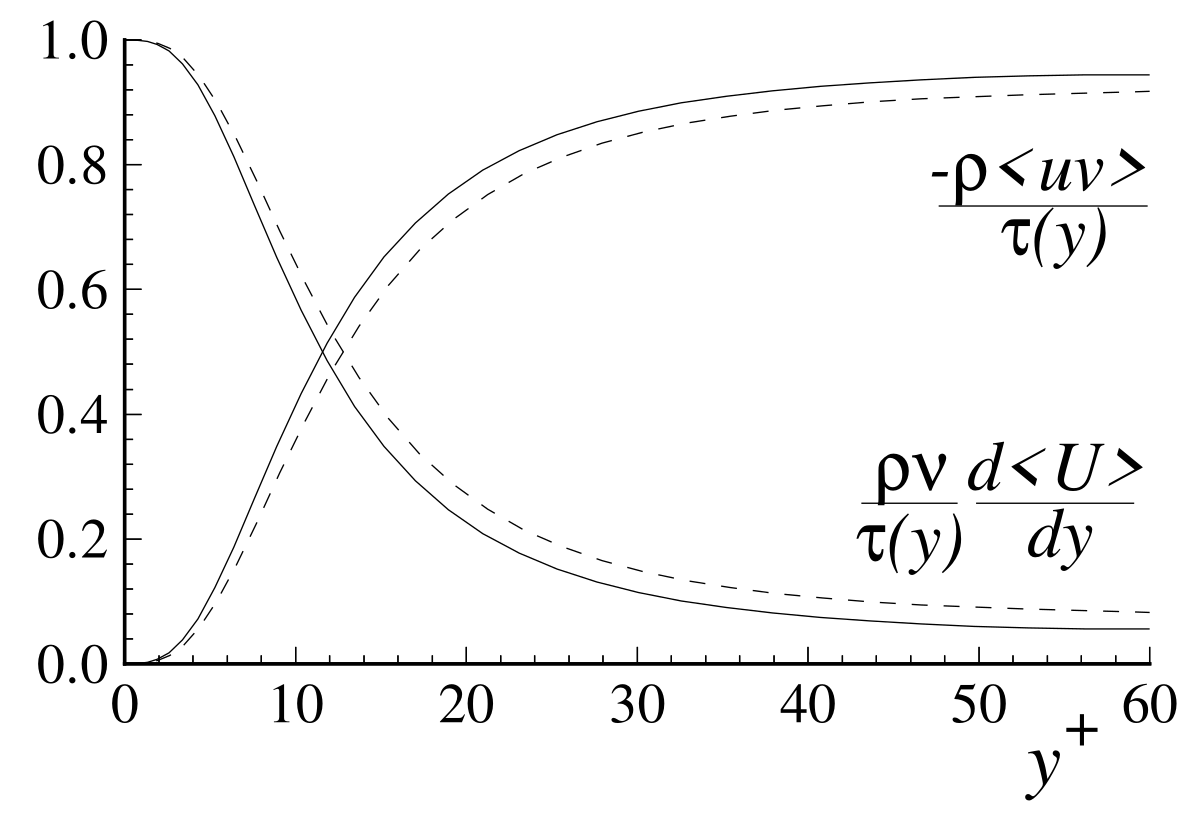
\includegraphics[width=0.6\textwidth]{assets/fig_channel_flow_stress_fractions.png}
  \caption{
    Profiles of the fractional contributions of the viscous and turbulent
    Reynolds stresses to the total stress, based on the DNS data of Kim et al.
    (1987), as in Figs. \ref{fig:channel_flow_turbulent_u} and
    \ref{fig:channel_flow_stress_profiles}.
    This is Figure 7.4 from Turbulent Flows by Pope.
  }
  \label{fig:channel_flow_stress_fractions}
\end{figure}

Based on the viscous length scale, we define a new non-dimensional coordinate
$z^+$ as:

\begin{equation}
  z^+ \equiv \frac{z}{\delta_\nu} = \frac{u_* z}{\nu}
\end{equation}
which is the physical vertical distance normalized by the viscous length scale.
This quantity thus allows us to see how the flow properties vary with the 
distance expressed as a number of wall units.
One example of that is the fractional contribution of the viscous and turbulent
stresses to the total stress, shown in Fig. \ref{fig:channel_flow_stress_fractions}.
The fact that the stress contribution profiles between the lower and higher
Reynolds number cases almost collapse on one another when plotted against $z^+$
(compare with the two cases in Fig. \ref{fig:channel_flow_stress_profiles})
provides a hint into the usefulness of this non-dimensionalization.
It demonstrates the universality of the turbulent flow structure, and allows us
to make some general statements about the flow structure that are independent of
the Reynolds number.
This figure shows that the viscous and turbulent stresses become approximately
equal at about $z^+ \approx 12$.
Some useful criteria for $z^+$ in characterizing the flow regimes are:

\begin{equation}
  z^+ \lesssim 5 \quad \text{(viscous sublayer)}
\end{equation}

\begin{equation}
  5 \lesssim z^+ \lesssim 50 \quad \text{(viscous wall region)}
\end{equation}

\begin{equation}
  z^+ \gtrsim 50 \quad \text{(outer region)}
\end{equation}

Let's now examine in more detail each of these regions and see if flow structure
varies significantly between them.

\subsection{Velocity structure in various wall regions}

Now, let's look at the time-mean velocity profiles in the turbulent channel flow,
and in various regions near and away from the wall.
When fully developed, such flow is completely determined by the fluid density
$\rho$, the kinematic viscosity $\nu$, the channel half-height $\delta$, and
the friction velocity $u_*$, because:

\begin{equation}
  u_* = \sqrt{- \frac{\delta}{\rho} \frac{\partial \overline{p}}{\partial x}}
\end{equation}
Between these parameters, there are only two independent non-dimensional groups
that can be formed: $z/\delta$ and $Re_\tau = u_* \delta / \nu$.
It should then be possible to express the velocity profile as a function of
these parameters:

\begin{equation}
  \overline{u}(z) = u_* F\left(\frac{z}{\delta}, Re_\tau\right)
\end{equation}
where $F$ is some yet-to-be-determined non-dimensional function.
However, since both the viscous stress and the turbulent production are determined
by the mean shear $\partial \overline{u}/\partial z$, it may be more useful to
seek the form of the velocity profile in terms of the mean shear:

\begin{equation}
  \frac{\partial \overline{u}}{\partial z} = \frac{u_*}{z} \Phi\left(\frac{z}{\delta}, \frac{z}{\delta_\nu}\right)
  \label{eq:law_of_wall1}
\end{equation}
where $\Phi$ is, like $F$ before, some yet-to-be-determined non-dimensional
function, and the proportionality to $u_*/z$ is proposed on dimensional grounds.
Notice that the second argument of $G$, $z/\delta_\nu$ (which we also defined
earlier as $z^+$), is equivalent to $Re_\tau z/\delta$, so it is useful to see
$G$ as a function of two non-dimensional heights, one characteristic of the
boundary layer and another of the viscous sublayer.

\begin{figure}[h]
  \centering
  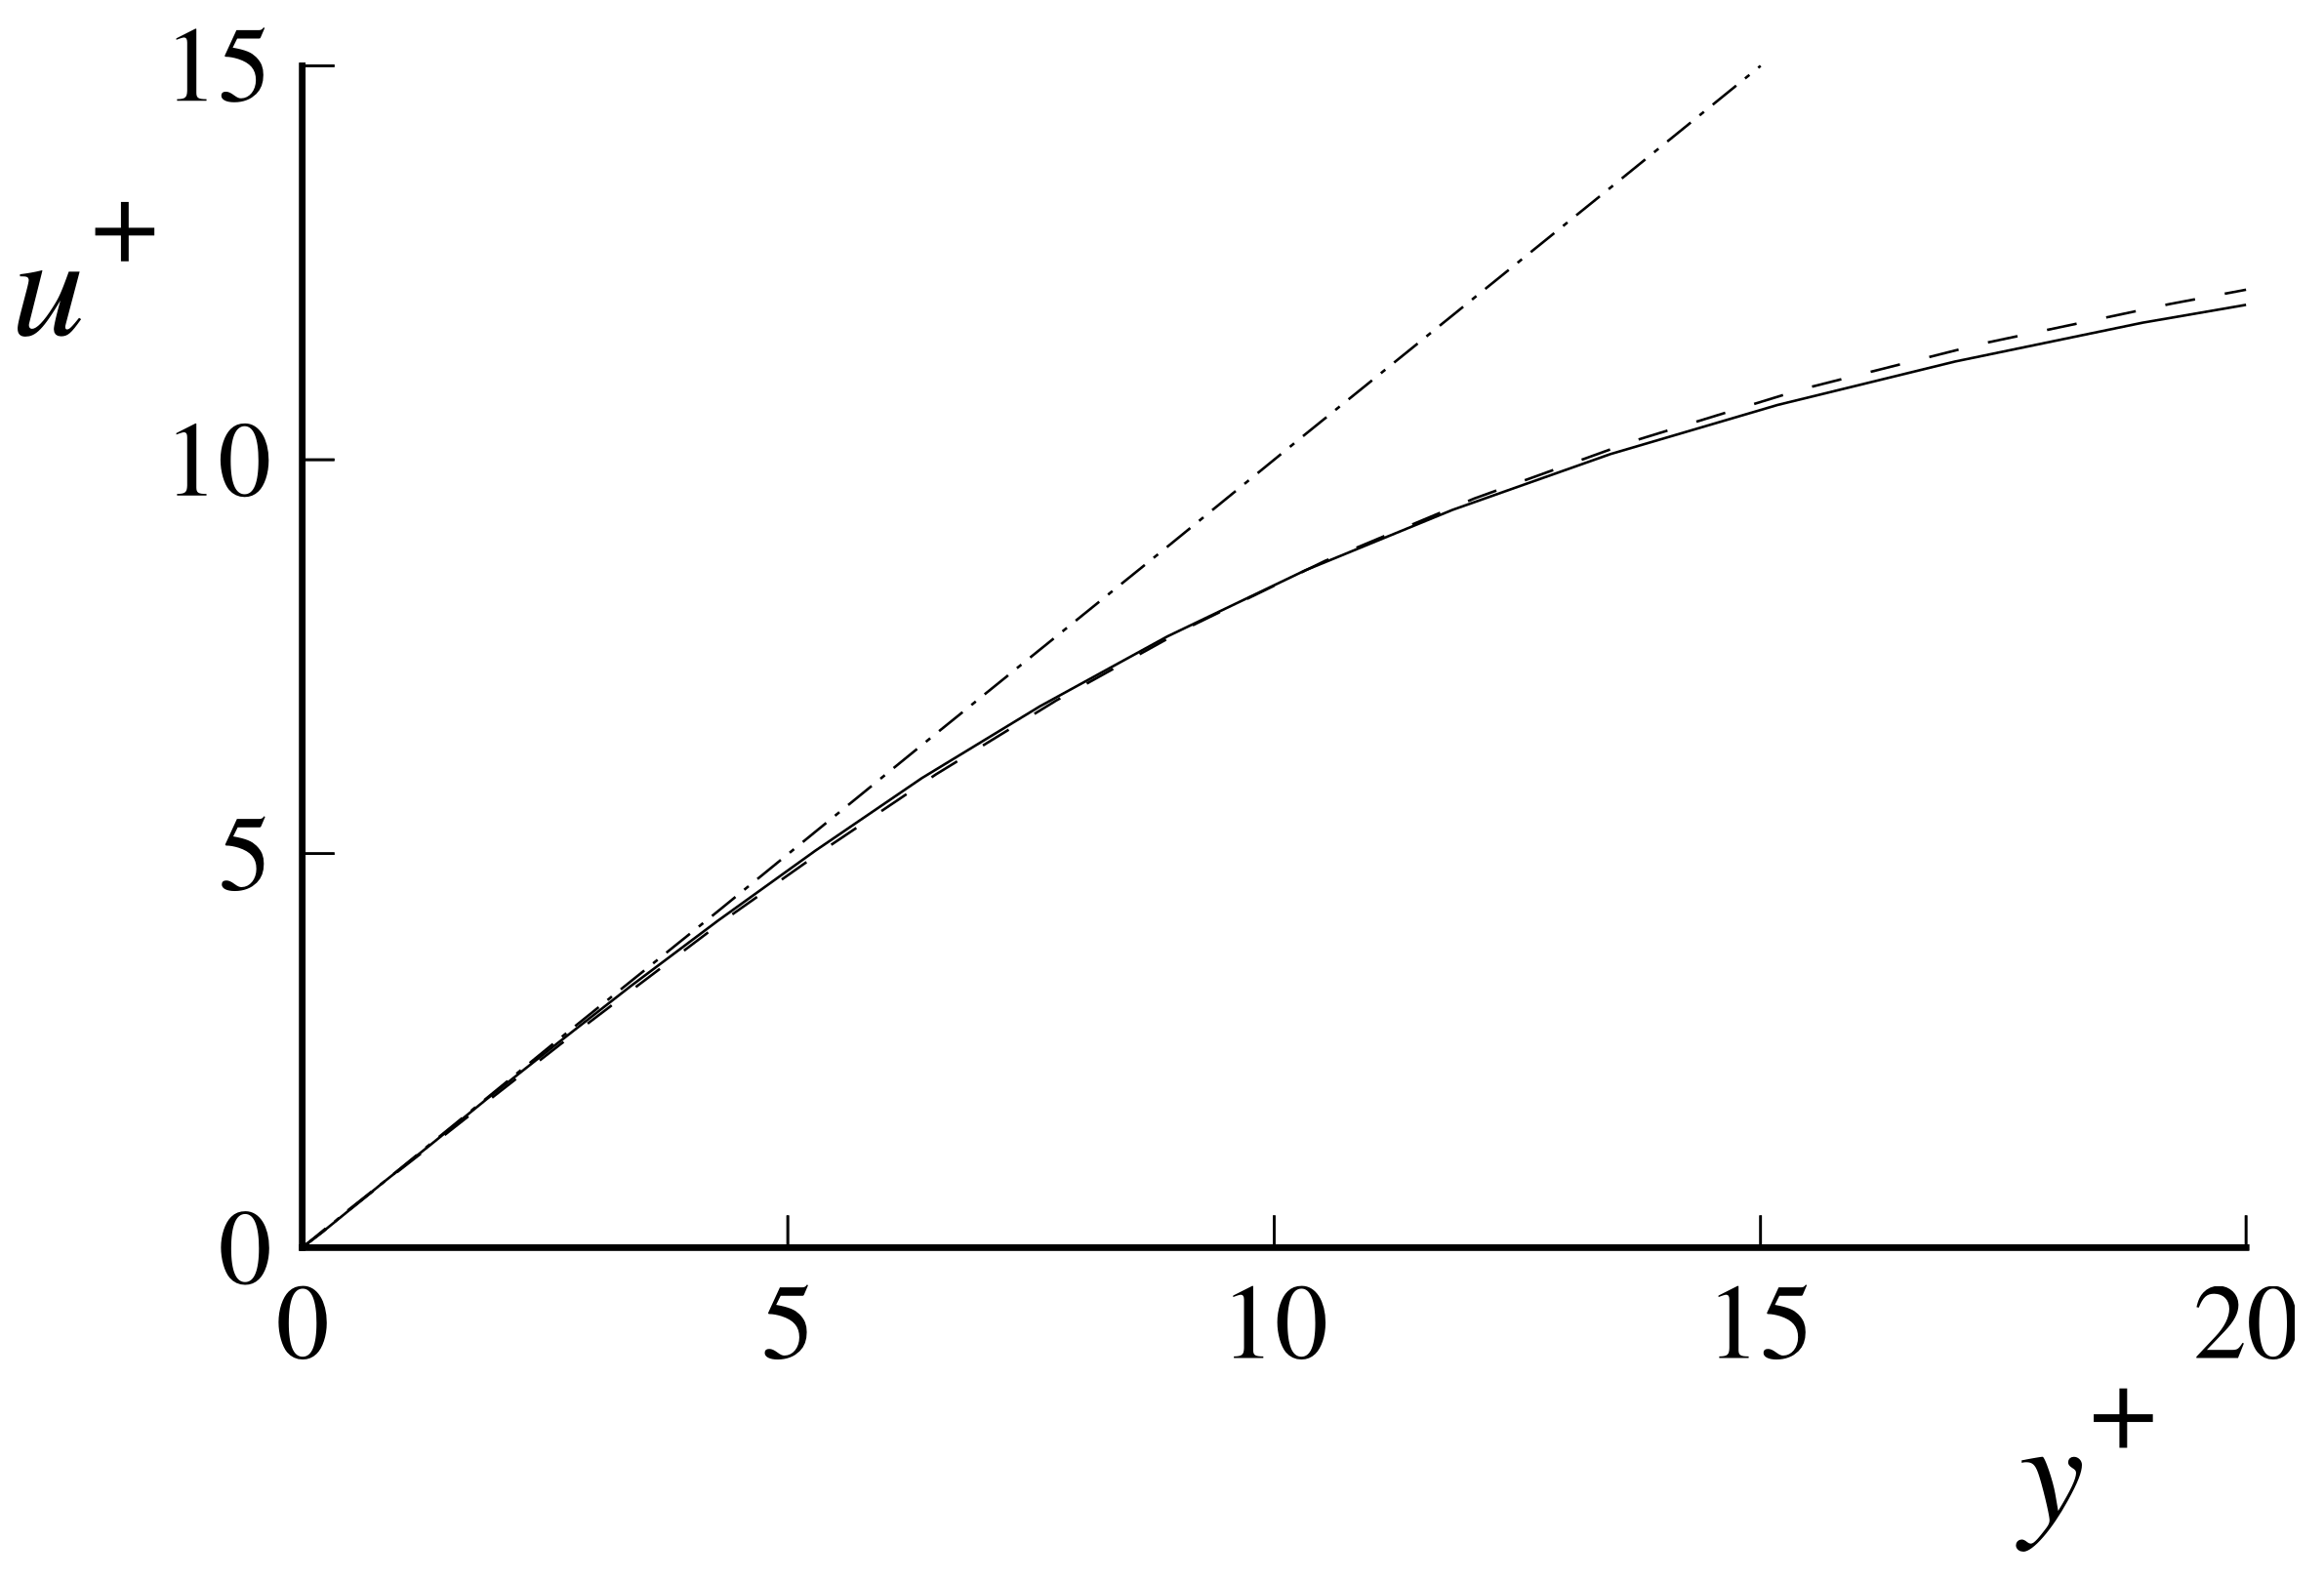
\includegraphics[width=0.6\textwidth]{assets/fig_law_of_the_wall_viscous_sublayer.png}
  \caption{
    Near-wall profiles of mean velocity from the DNS data of Kim et al. (1987):
    dashed line, $Re = 5,600$; solid line, $Re = 13,750$; dot-dashed line,
    $u^+ = z^+$.
    This is Figure 7.5 from Turbulent Flows by Pope.
  }
  \label{fig:law_of_the_wall_viscous_sublayer}
\end{figure}

Let's focus for now on the region closest to the wall, which may include the
viscous sublayer and extend somewhat beyond it.
Prandtl (1925) hypothesized that at high Reynolds numbers, there is a region
very near the wall ($z \ll \delta$), called the \textit{inner layer}, in which
the mean velocity profile is entirely governed by viscosity, and is independent
of the boundary layer size $\delta$ and the centerline velocity $u_0$.
Thus, as $z/\delta \to 0$, $\Phi(z/\delta, z/\delta_\nu) \to \Phi_I(z/\delta_\nu)$,
so in this region Eq. (\ref{eq:law_of_wall1}) reduces to:

\begin{equation}
  \frac{\partial \overline{u}}{\partial z} =
  \frac{u_*}{z} \Phi_I\left(\frac{z}{\delta_\nu}\right) =
  \frac{u_*}{z} \Phi_I\left(z^+\right)
  \label{eq:law_of_wall2}
\end{equation}
Since $\Phi_I$ is a function of $z^+$ and it's the function that we want to
determine, let's express the other variables in Eq. (\ref{eq:law_of_wall2}) in
terms of $z^+$ as well.
To do that, we introduce the non-dimensional velocity which is the velocity
normalized by the friction velocity:

\begin{equation}
  u^+ \equiv \frac{\overline{u}}{u_*}
\end{equation}
Recalling that $u_* = \nu/\delta_\nu$ and that $z^+ = z/\delta_\nu$, we can
express Eq. (\ref{eq:law_of_wall2}) as:

\begin{equation}
  \frac{\partial u^+}{\partial z^+} = \frac{1}{z^+} \Phi_I\left(z^+\right)
  \label{eq:law_of_wall3}
\end{equation}
The non-dimensional velocity $u^+$ is thus a function of $z^+$ alone:

\begin{equation}
  u^+ = f_w(z^+)
  \label{eq:law_of_wall4}
\end{equation}
where $f_w$ is the \textit{wall function}\index{Wall!Function}, expressed in
terms of $z^+$ as:

\begin{equation}
  f_w(z^+) = \int_0^{z^+} \Phi_I(z) dz
  \label{eq:law_of_wall5}
\end{equation}
Equations (\ref{eq:law_of_wall4})-(\ref{eq:law_of_wall5}) make the so-called
\textit{law of the wall}\index{Wall!Law of the}.
There is copious experimental and DNS evidence that $f_w(z^+)$ is a universal
function for boundary layers in general.
Let's find the form of this function for small and large values of $z^+$.

In the viscous sublayer, we can establish from Eq. (\ref{eq:wall_stress}) and
the no slip boundary condition that:

\begin{equation}
  f_w(0) = 0
\end{equation}

\begin{equation}
  f'_w(0) = 1
\end{equation}
which implies that for very small values of $z^+$, the wall function is:

\begin{equation}
  f_w(z^+) \approx z^+
  \label{eq:law_of_wall6}
\end{equation}

The validity of the linear scaling of the velocity with $z^+$ in the inner layer
is shown based on DNS data in Fig. \ref{fig:law_of_the_wall_viscous_sublayer}.
Up to about $z^+ \approx 5$, the velocity scales linearly with $z^+$, as expected
from the viscous sublayer.
However, beyond $z^+ \approx 5$, the velocity scales differently and we need
to seek a different functional form for $f_w(z^+)$.
Based on the data, it seems like the function may have a logarithmic dependence
on $z^+$.

\begin{figure}[h]
  \centering
  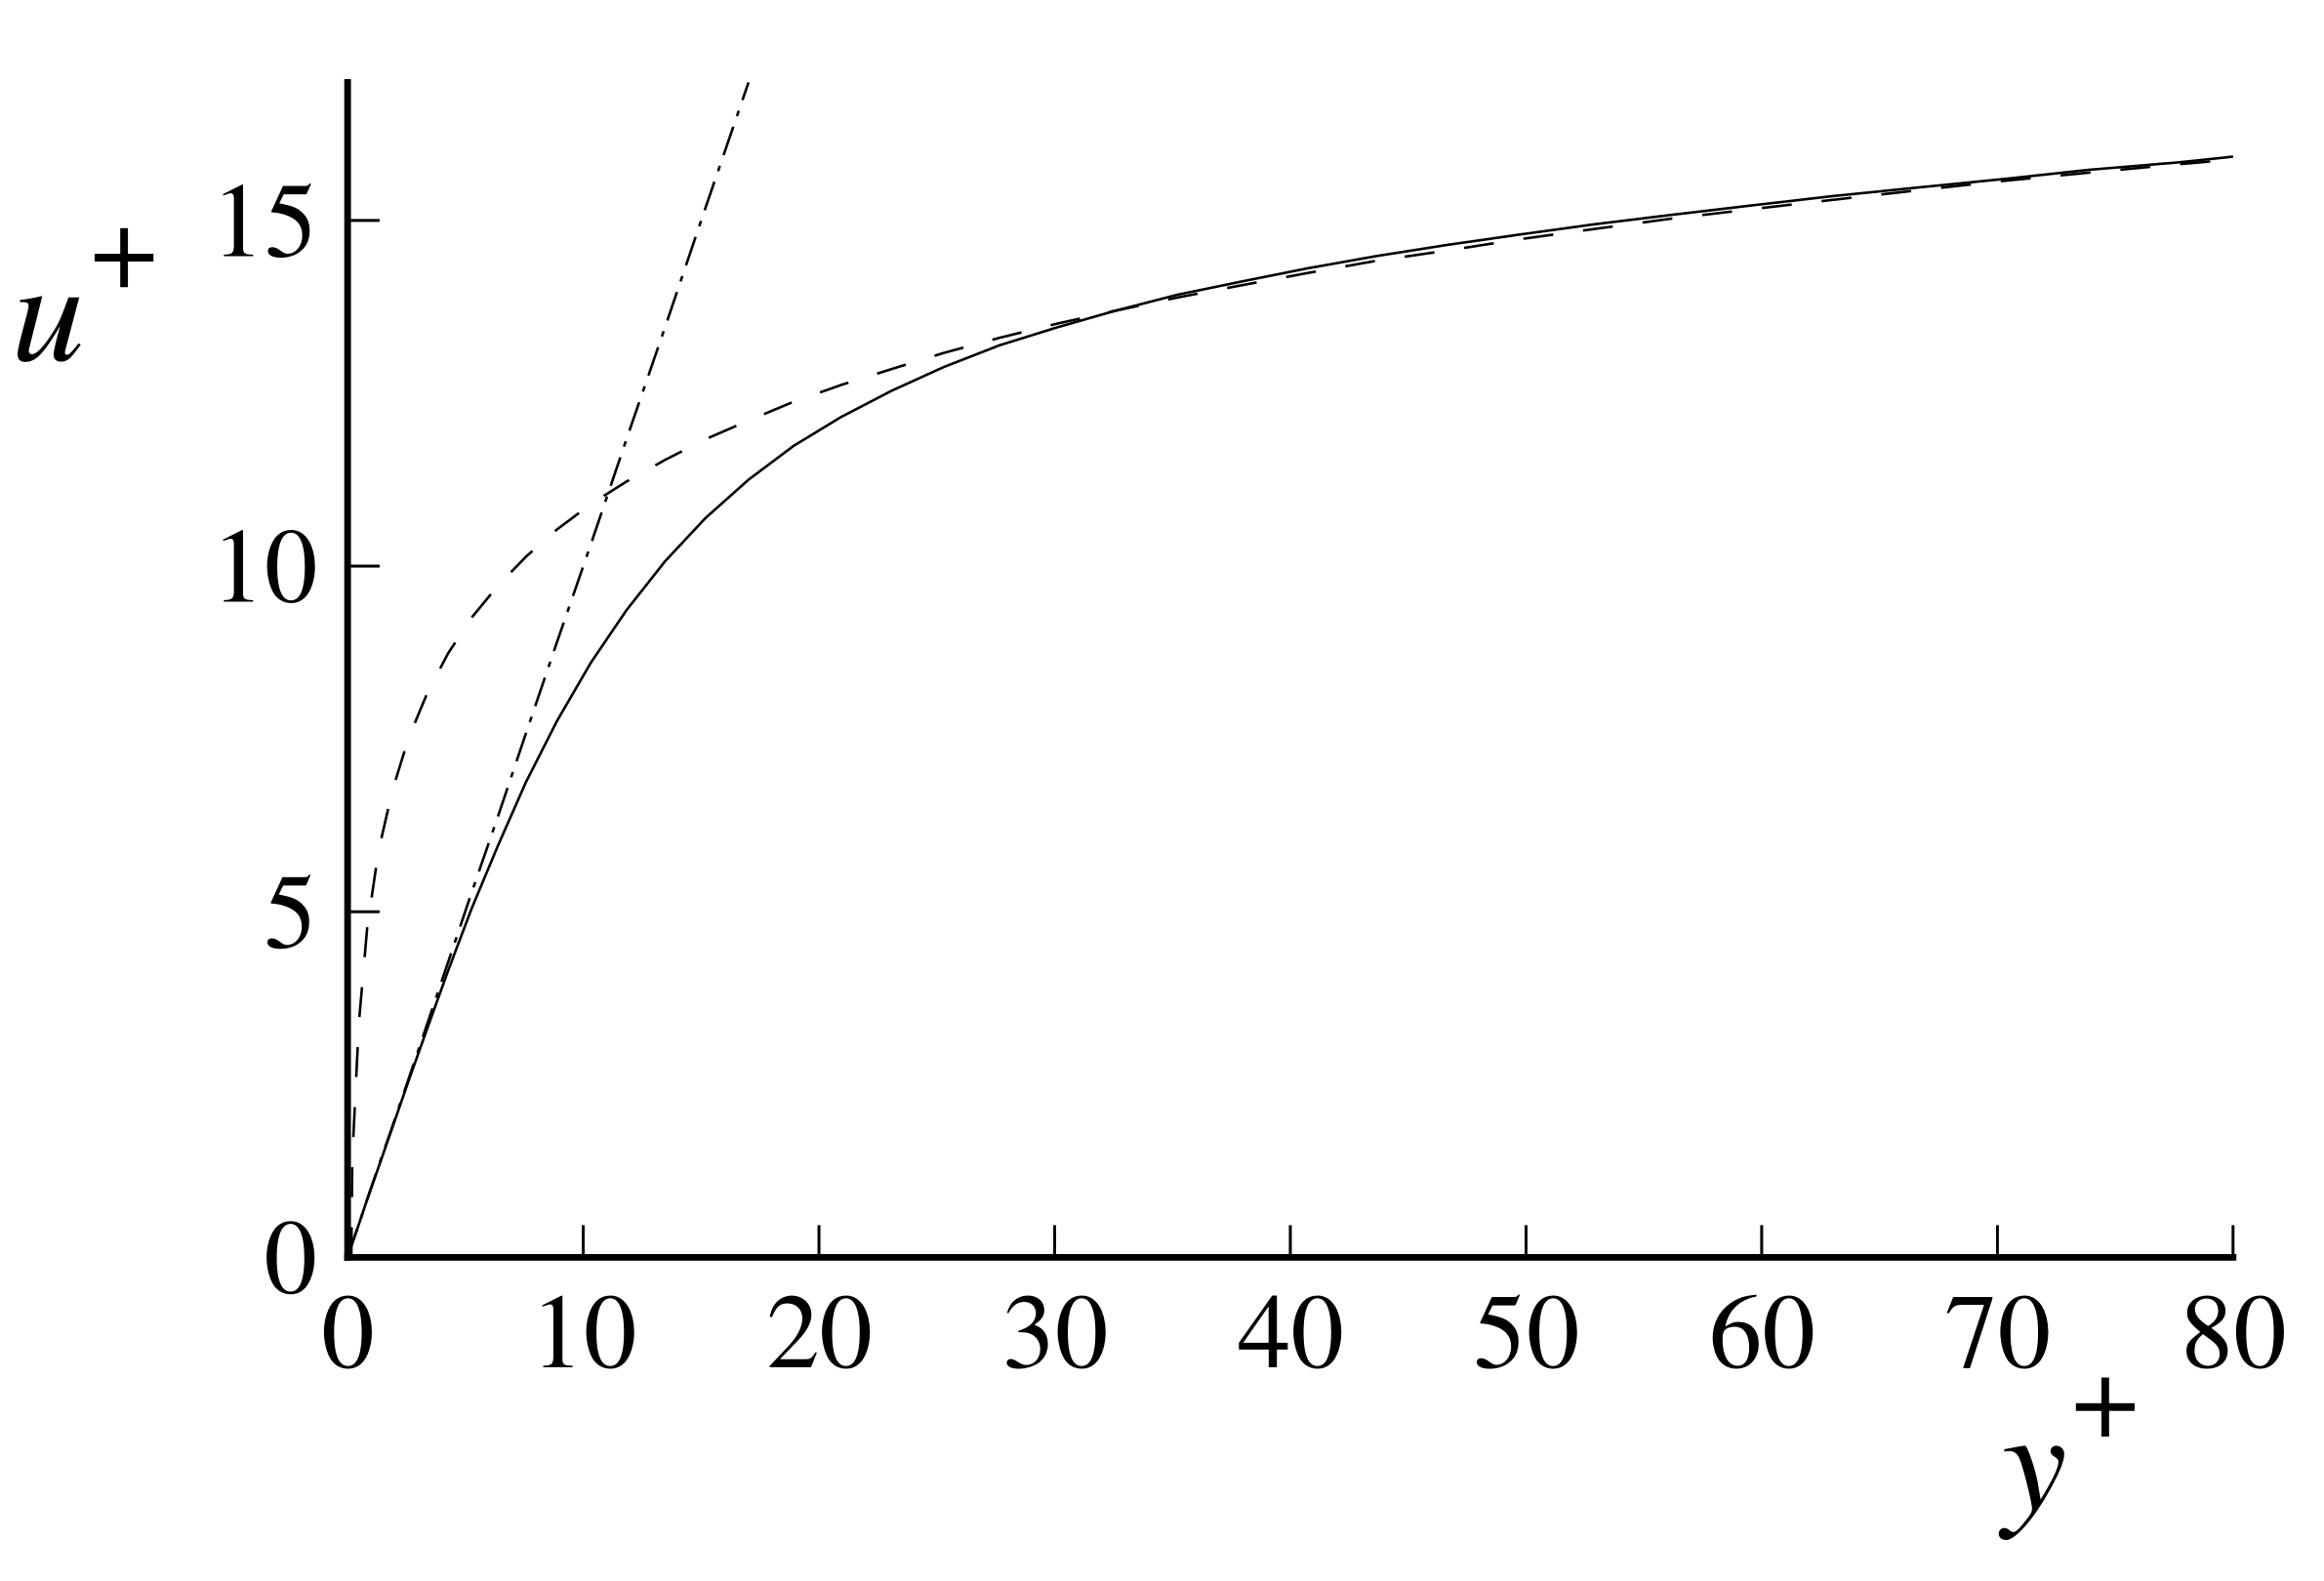
\includegraphics[width=0.6\textwidth]{assets/fig_law_of_the_wall_loglaw.png}
  \caption{
    Near-wall profiles of mean velocity:
    Solid line, DNS data of Kim et al. (1987), $Re = 13,750$;
    dot-dashed line, $u^+ = z^+$; dashed line, the log-law.
    This is Figure 7.6 from Turbulent Flows by Pope.
  }
  \label{fig:law_of_the_wall_loglaw}
\end{figure}

Away from the wall, we can suppose that the viscosity plays smaller role, and
thus $\Phi_I(z^+)$ reduces to a constant, experimentally determined to be
$1/\kappa$, where $\kappa$ is the von Kármán constant and approximately equal to
$0.41$:

\begin{equation}
  \Phi_I(z^+) = \frac{1}{\kappa}, \quad \text{for } \frac{z}{\delta} \ll 50   \text{ and } z^+ \gg 1
\end{equation}
In this region, the velocity shear is then:

\begin{equation}
  \frac{\partial u^+}{\partial z^+} = \frac{1}{\kappa z^+}
\end{equation}
which integrates to:

\begin{equation}
  u^+ = \frac{1}{\kappa} \ln(z^+) + C
  \label{eq:law_of_the_wall_loglaw}
\end{equation}
where $C$ is an integration constant, experimentally determined to be about $5.2$.
Returning back to our dimensional variables, we can express the velocity profile
as:

\begin{equation}
  \overline{u}(z) = u_* \left[ \frac{1}{\kappa} \ln\left(\frac{z}{\delta_\nu}\right) + 5.2 \right]
  \label{eq:law_of_the_wall_loglaw_dim}
\end{equation}

The log-law is demonstrated based on DNS data in Fig. \ref{fig:law_of_the_wall_loglaw},
and its universality (\textit{i.e.} independence of the Reynolds number) is
demonstrated based on experimental data in Fig. \ref{fig:law_of_the_wall_measurements}.

\begin{figure}[h]
  \centering
  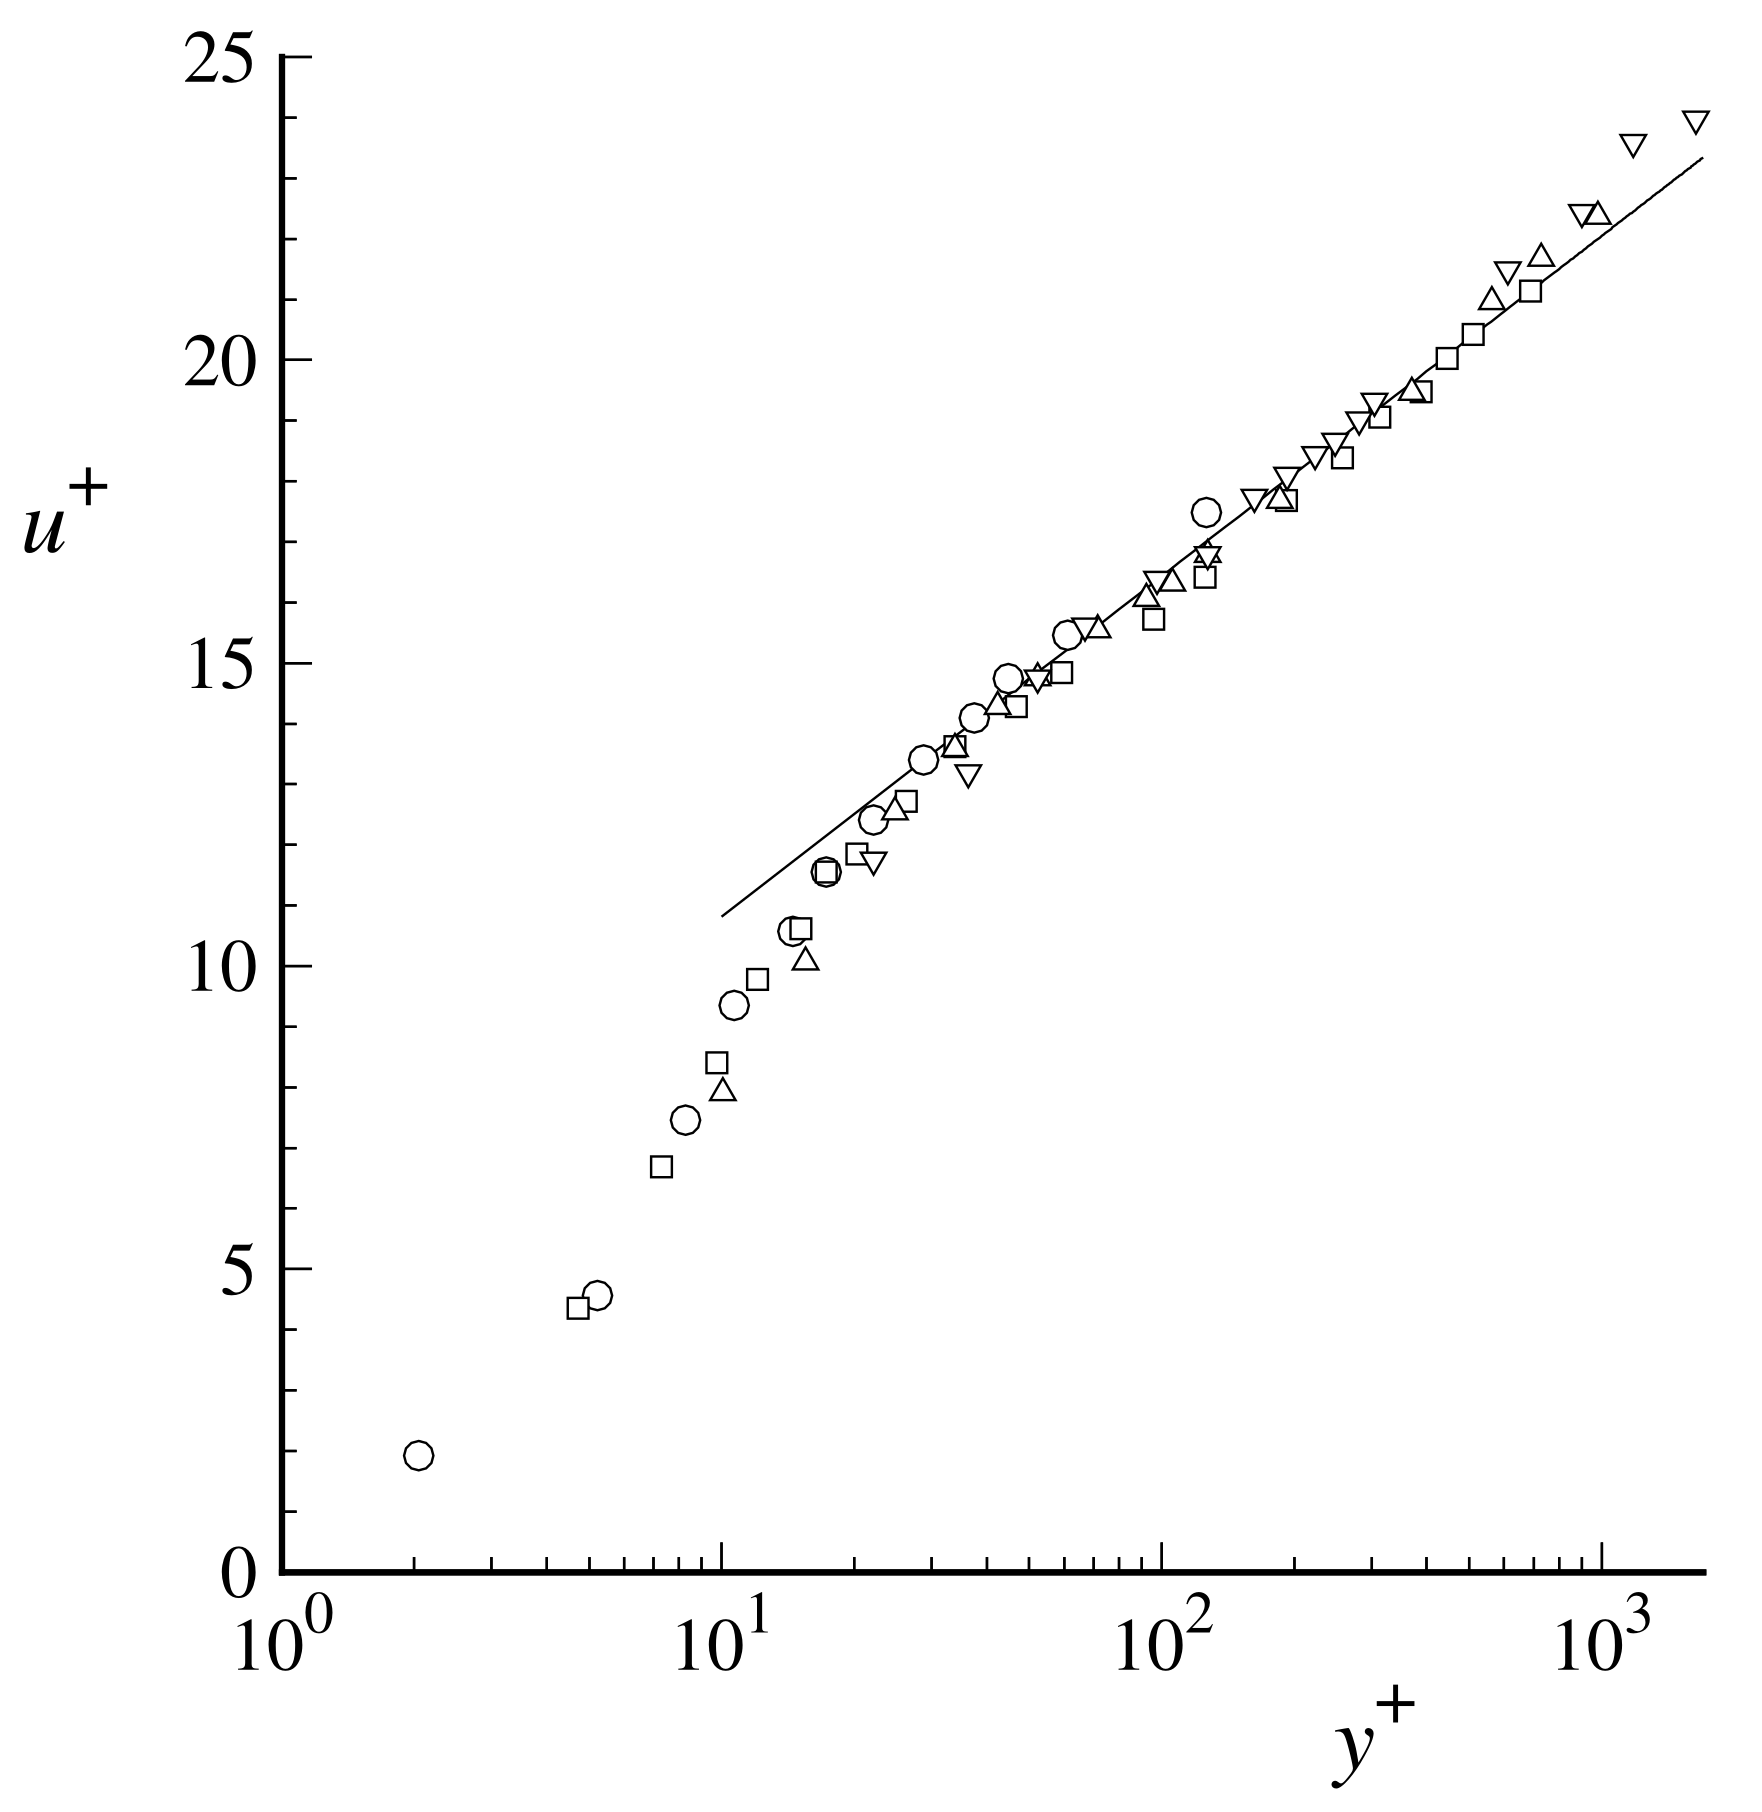
\includegraphics[width=0.6\textwidth]{assets/fig_law_of_the_wall_measurements.png}
  \caption{
    Mean velocity profiles in fully developed turbulent channel flow measured by
    Wei and Willmarth (1989):
    Circles, $Re_0 = 2,970$; squares, $Re_0 = 14,914$; upward triangles, $Re_0 = 22,776$;
    downward triangles, $Re_0 = 39,582$; line, the log-law.
    This is Figure 7.7 from Turbulent Flows by Pope.
  }
  \label{fig:law_of_the_wall_measurements}
\end{figure}

%\begin{figure}[h]
%  \centering
%  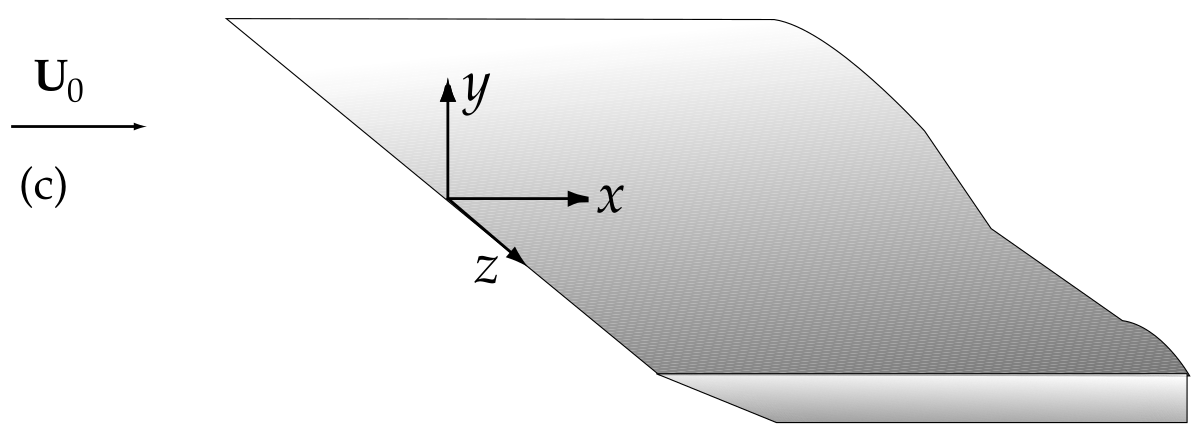
\includegraphics[width=0.8\textwidth]{assets/fig_wall_flow.png}
%  \caption{
%    Flow over a flat plate, with the mean flow velocity $U_0$ at the top of the
%    boundary layer.
%    Note the notation reversal from the main text, where $z$ is the vertical
%    coordinate.
%    This is Figure 7.1c from Turbulent Flows by Pope.
%  }
%  \label{fig:wall_flow}
%\end{figure}

\subsection{Exercises}

\begin{enumerate}
  \item Find the expression for the bulk velocity (see Eq. \ref{eq:bulk_velocity})
  of a laminar channel flow. How large is it compared to the centerline velocity
  $u_0$? How about the bulk Reynolds number relative to the centerline Reynolds
  number $Re_0$?
  \item Consider a fully developed turbulent channel flow at $Re = 10^5$ (Eq. \ref{eq:Re_bulk}).
  The fluid is water with $\rho = 10^3$ kg/m$^3$ and viscosity $\nu = 10^{-6}$ m$^2$/s.
  The channel half-height is $\delta = 0.1$ m,
  and the skin-friction coefficient is $C_f = u_*^2 / U_0^2 = 4 \times 10^{-3}$.
  Find the bulk velocity $\left< \overline{u} \right>$, the friction velocity $u_*$,
  the friction Reynolds number $Re_\tau$, and the viscous length scale $\delta_\nu$.
\end{enumerate}

\subsection*{Further reading}

\begin{itemize}
  \item Chapter 7 of Turbulent Flows by Stephen Pope.
\end{itemize}

\newpage
\section{Surface gravity waves}
\label{sec:surface_gravity_waves}

In this chapter, we examine in detail the boundary between the atmosphere and
the ocean, that is, the surface waves.
The key restoring force for the surface waves, as we will soon see, is gravity,
and so these waves are often called \textit{gravity waves}\index{Gravity waves},
much like the waves we explored as a solution of the shallow water equations in
Chapter \ref{sec:shallow_water_systems}.
In the first part of this chapter, we derive the solution for the
small-amplitude (also often called linear) waves, which are valid when the
wave amplitude is much smaller than the wavelength and the water depth.
This assumption allows for a relatively straightforward solution of the flow
anywhere below the free wavy surface.
Although simplistic in its approximations, the linear wave theory has been
surprisingly successful in predicting the behavior of the waves even when the
assumptions behind it are clearly violated.
The linear wave theory remains the basis of modern wave prediction models that
are used in operational weather and ocean forecasting.
After deriving the linear wave solutions, we will explore their properties
and derive some second-order quantities with implication on mean ocean
circulation.

\subsection{Small-amplitude wave derivation}

\subsubsection{Governing equations}
\label{sec:governing_equations}
Key assumptions are that the fluid is incompressible
($\nabla \cdot \mathbf{u} = 0$), inviscid ($\nu \nabla^2 \mathbf{u} = 0$),
and irrotational ($\nabla \times \mathbf{u} = 0$).
Velocity $\mathbf{u}$ then has a scalar potential $\phi$ such that:

\begin{equation}
  \mathbf{u} = \nabla \phi =
  \frac{\partial \phi}{\partial x} \mathbf{i} +
  \frac{\partial \phi}{\partial y} \mathbf{j} +
  \frac{\partial \phi}{\partial z} \mathbf{k}
\end{equation}
Incompressibility then dictates that:

\begin{equation}
  \nabla \cdot \nabla \phi = \nabla^2 \phi = 0
  \label{eq:laplace}
\end{equation}
This is called the Laplace equation, and it holds throughout the fluid.
In two dimensions, horizontal and vertical, Eq. (\ref{eq:laplace}) is:

\begin{equation}
  \frac{\partial^2 \phi}{\partial x^2} + \frac{\partial^2 \phi}{\partial z^2} = 0
  \label{eq:laplace_2d}
\end{equation}
which is sufficient if we consider surface waves that propagate in the
$x$-direction and that are otherwise uniform in the $y$-direction.

Although $\phi$ is allowed to vary in both space and time, the Laplace equation
states that at any given time, $\phi$ anywhere in the interior of the fluid is
determined by its values at the boundary (\textit{i.e.} the boundary conditions).
It does not, however, determine how $\phi$ evolves in time.
One important property of the velocity potential is that it is not unique,
\textit{i.e.} there are infinitely many functions that satisfy the Laplace
equation.
For example, if $\phi$ is a velocity potential, then so is $\phi + C$, where $C$
is a scalar constant, and so is $\phi + f(t)$, where $f(t)$ is an arbitrary
function of time.
Another one is that a sum of any number of velocity potentials is also a
velocity potential.

Now, to determine the time dependence of $\phi$, we can integrate the Euler
equations of motion (introduced back in Section \ref{sec:momentum}, see
Eq. \ref{eq:momentum_euler}) to obtain a steady-state relationship between the
pressure and the velocity of the fluid.
The Euler equations in $x$-$z$ plane are:

\begin{equation}
  \frac{\partial u}{\partial t} +
  u \frac{\partial u}{\partial x} +
  w \frac{\partial u}{\partial z} =
  - \frac{1}{\rho} \frac{\partial p}{\partial x}
  \label{eq:euler_x}
\end{equation}

\begin{equation}
  \frac{\partial w}{\partial t} +
  u \frac{\partial w}{\partial x} +
  w \frac{\partial w}{\partial z} =
  - \frac{1}{\rho} \frac{\partial p}{\partial z}
  - g
  \label{eq:euler_z}
\end{equation}
Now, recall that we require the flow to be irrotational, so:

\begin{equation}
  \omega = \frac{\partial w}{\partial x} - \frac{\partial u}{\partial z} = 0
\end{equation}
which leads to:

\begin{equation}
  \frac{\partial w}{\partial x} = \frac{\partial u}{\partial z}
\end{equation}
We can use this to rewrite Eqs. (\ref{eq:euler_x})-(\ref{eq:euler_z}) as:

\begin{equation}
  \frac{\partial u}{\partial t} +
  \frac{1}{2} \left( \frac{\partial u^2}{\partial x} + \frac{\partial w^2}{\partial x} \right) =
  - \frac{1}{\rho} \frac{\partial p}{\partial x}
\end{equation}

\begin{equation}
  \frac{\partial w}{\partial t} +
  \frac{1}{2} \left( \frac{\partial u^2}{\partial z} + \frac{\partial w^2}{\partial z} \right) =
  - \frac{1}{\rho} \frac{\partial p}{\partial z} - g
\end{equation}
Now, express the velocity components in the time derivatives as gradients of the
velocity potential:

\begin{equation}
  \frac{\partial}{\partial x} \left[
    \frac{\partial \phi}{\partial t} +
    \frac{1}{2} \left(u^2 + w^2\right) +
    \frac{p}{\rho}
  \right] = 0
\end{equation}

\begin{equation}
  \frac{\partial}{\partial z} \left[
    \frac{\partial \phi}{\partial t} +
    \frac{1}{2} \left(u^2 + w^2\right) +
    \frac{p}{\rho}
  \right] = -g
\end{equation}
Integrating these equations with respect to $x$ and $z$ respectively, we obtain:

\begin{equation}
  \frac{\partial \phi}{\partial t} +
  \frac{1}{2} \left(u^2 + w^2\right) +
  \frac{p}{\rho} = C'(z, t)
\end{equation}

\begin{equation}
  \frac{\partial \phi}{\partial t} +
  \frac{1}{2} \left(u^2 + w^2\right) +
  \frac{p}{\rho} = C(x, t) - gz
\end{equation}
where $C(x, t)$ and $C'(z, t)$ are integration constants that can vary in
dimensions other than their respective dimension of integration.
Since these equations have the same left-hand sides, their right-hand sides must
be equal:

\begin{equation}
  C(x, t) = C'(z, t) + gz
\end{equation}
$C(x, t)$ thus can only depend on time, and we get our final equation form
called the \textit{Bernoulli equation}\index{Bernoulli equation}:

\begin{equation}
  \frac{\partial \phi}{\partial t} +
  \frac{1}{2} \left(u^2 + w^2\right) +
  \frac{p}{\rho} + gz= C(t)
  \label{eq:bernoulli}
\end{equation}
The Bernoulli equation will serve as a dynamic free surface boundary condition
as we proceed to derive the solutions for the surface gravity waves.

\subsubsection{Boundary conditions}
\label{sec:boundary_conditions}

Now that we established the governing equations to solve, we need to specify the
boundary conditions to determine the velocity potential in the interior.
We will rely on a total of four boundary conditions:

\begin{enumerate}
  \item \textbf{Kinematic free surface boundary condition}:
  This boundary condition determines the vertical velocity at the free surface
  $\eta(x, t)$ by exploiting the fact that the Lagrangian (material) change of
  the vertical position is the vertical velocity itself:
  \begin{equation}
    w = \frac{dz}{dt}\Big|_{z=\eta} = \frac{\partial \eta}{\partial t} + u \frac{\partial \eta}{\partial x}
  \end{equation}
  Expressed in terms of the velocity potential, this boundary condition becomes:
  \begin{equation}
    \frac{\partial \phi}{\partial z} =
    \frac{\partial \eta}{\partial t} +
    \frac{\partial \phi}{\partial x} \frac{\partial \eta}{\partial x}, \text{ at } z=\eta(x, t)
  \end{equation}
  \item \textbf{Dynamic free surface boundary condition}:
  We leverage the Bernoulli equation (Eq. \ref{eq:bernoulli}) at the free surface
  ($z = \eta$) and set the surface pressure to be zero:
  \begin{equation}
    \frac{\partial \phi}{\partial t} + \frac{1}{2} \left(u^2 + w^2\right) + g\eta = C(t), \text{ at } z=\eta(x, t)
  \end{equation}
  \item \textbf{Bottom boundary condition}:
  The bottom is rigid and impermeable, so the vertical velocity is zero at the
  bottom:
  \begin{equation}
    w = 0, \text{ at } z = -h
  \end{equation}
  where $h$ is the mean depth of the fluid.
  \item \textbf{Lateral boundary condition}:
  At the lateral boundaries, since we're seeking a wave solution, we know that
  the velocity potential must be periodic in the horizontal space as well as
  time:
  \begin{equation}
    \phi(x, t) = \phi(x+L, t)
  \end{equation}
  \begin{equation}
    \phi(x, t) = \phi(x, t+T)
  \end{equation}
  where $L$ is the wavelength and $T$ is the period.
\end{enumerate}
With these four boundary conditions, we are now equipped to solve for the velocity
potential in the interior of the fluid.

\subsubsection{Solution}

Our key equation to solve is the Laplace equation (Eq. \ref{eq:laplace})
for the velocity potential $\phi$ that varies in the horizontal and vertical
direction $x$ and $z$ respectively, as well as time $t$:

\begin{equation}
  \nabla^2 \phi(x, z, t) = 0
  \label{eq:laplace2}
\end{equation}
To solve this equation, we will rely on the method of separation of variables,
where we assume that the solution can be written as a product of functions that
depend on each coordinate separately:

\begin{equation}
  \phi(x, z, t) = \phi_x(x) \phi_z(z) \phi_t(t)
\end{equation}
We can start from the time-dependent part $\phi_t(t)$ and recall the lateral
boundary condition which states that the velocity potential must be periodic
in time, which is true for sines and cosines (and some combinations of them).
For a sine function of a phase $\varphi$, this is true:

\begin{equation}
  \sin(\varphi) = \sin(\varphi + 2\pi)
\end{equation}
And expressing it as a function of time:

\begin{equation}
  \sin(\omega t) = \sin(\omega t + 2\pi)
\end{equation}
where $\omega$ is the angular frequency in units of radians per second, so that
the phase $\varphi$ has angle units (radians).
Notice that we could have picked (and soon, we will) a cosine function instead of
a sine function, and the solution would be still be valid.
With the choice of a sine for the time-dependent part of the potential, we write
the full velocity potential as:

\begin{equation}
  \phi(x, z, t) = \phi_x(x) \phi_z(z) \sin(\omega t)
  \label{eq:phi1}
\end{equation}
Insert this into Eq. (\ref{eq:laplace2}) to get:

\begin{equation}
  \frac{\partial^2 \phi_x}{\partial x^2} \phi_z \sin(\omega t) +
  \phi_x \frac{\partial^2 \phi_z}{\partial z^2} \sin(\omega t) = 0
\end{equation}
Divide by $\phi_x \phi_z \sin(\omega t)$ to get:

\begin{equation}
  \frac{1}{\phi_x} \frac{\partial^2 \phi_x}{\partial x^2} +
  \frac{1}{\phi_z} \frac{\partial^2 \phi_z}{\partial z^2} = 0
  \label{eq:phi2}
\end{equation}
Can we separate this even further?
Recall that $\phi_x$ and $\phi_z$ are functions of $x$ and $z$ respectively.
If, for example, we hold $x$ constant and consider variations in $z$, the
first term would remain constant but the second term would not!
You can arrive to the same conclusion by holding $z$ constant and varying $x$.
This would clearly violate Eq. (\ref{eq:phi2}), and so the only way that
equation can hold is if both $\phi_x$ and $\phi_z$ are equal to the same
constant but with opposite signs:

\begin{equation}
  \frac{1}{\phi_x} \frac{\partial^2 \phi_x}{\partial x^2} = -k^2
  \label{eq:phi3}
\end{equation}

\begin{equation}
  \frac{1}{\phi_z} \frac{\partial^2 \phi_z}{\partial z^2} = k^2
  \label{eq:phi4}
\end{equation}
where $k$ is the separation constant.
These can also be written as:

\begin{equation}
  \frac{\partial^2 \phi_x}{\partial x^2} + k^2 \phi_x = 0
  \label{eq:phi5}
\end{equation}

\begin{equation}
  \frac{\partial^2 \phi_z}{\partial z^2} - k^2 \phi_z = 0
  \label{eq:phi6}
\end{equation}
For real values of $k$, the solutions to these equations are:

\begin{equation}
  \phi_x(x) = A \sin(kx) + B \cos(kx)
\end{equation}

\begin{equation}
  \phi_z(z) = C e^{kz} + D e^{-kz}
  \label{eq:phi_z}
\end{equation}
where $A$, $B$, $C$, and $D$ are constants that are yet to be determined.
We now write our intermediate solution for the velocity potential as:

\begin{equation}
  \phi(x, z, t) = \left[ A \sin(kx) + B \cos(kx) \right] \left[ C e^{kz} + D e^{-kz} \right] \sin(\omega t)
  \label{eq:phi_inter}
\end{equation}

Next, let's attempt to constrain the $z$-dependent part of the potential,
$\phi_z(z) = C e^{kz} + D e^{-kz}$.
Recall the bottom boundary condition which for a flat bottom requires $w = 0$
at $z = -h$.
Then:

\begin{equation}
  w = \frac{\partial \phi_z}{\partial z} = k \left( C e^{kz} - D e^{-kz} \right) = 0
\end{equation}
which implies $C = D e^{2kh}$.
Insert this back into Eq. (\ref{eq:phi_z}) to get:

\begin{equation}
  \begin{split}
    \phi_z(z) &=
    D \left( e^{2kh} e^{kz} + e^{-kz} \right) \\
    &=
    2 D e^{kh} \left( e^{k(z+h)} + e^{-k(z+h)} \right) \\
    &=
    2 D e^{kh} \cosh\left( k(z+h) \right)
  \end{split}
\end{equation}
Inserting this back into Eq. (\ref{eq:phi_inter}) we get:

\begin{equation}
  \phi(x, z, t) = \left[ A \sin(kx) + B \cos(kx) \right] 2 D e^{kh} \cosh\left( k(z+h) \right) \sin(\omega t)
  \label{eq:phi_inter2}
\end{equation}

Now, how about the free surface boundary condition?
Recall the Bernoulli equation at $z = \eta$ with $p = 0$:

\begin{equation}
  \frac{\partial \phi}{\partial t} + \frac{1}{2} \left(u^2 + w^2\right) + g\eta = C(t), \text{ at } z=\eta(x, t)
  \label{eq:bernoulli_free_surface}
\end{equation}
If we denote this equation as BE, we could evaluate it at the free surface
$z = \eta$ using a Taylor expansion around $z = 0$:

\begin{equation}
  BE_{z=\eta} = BE_{z=0} +
  \eta \frac{\partial{BE}}{\partial z} +
  \frac{1}{2} \eta^2 \frac{\partial^2{BE}}{\partial z^2} + \cdots
\end{equation}
To greatly simplify the algebra, this is where we invoke the small-amplitude
approximation, which effectively states that if $\eta \ll 1$, then 
$\eta^2 \ll \eta$, $\eta \ll u \eta$, $u \ll u^2$, and so on.
This is where the \textit{linearization} of the wave solution occurs, and it's
where it is possible to find wave solutions to a higher-order, such as those
of the Stokes wave theory.
For brevity, we keep only the first-order terms being the largest and write:

\begin{equation}
  \left( \frac{\partial \phi}{\partial t} + g\eta \right)_{z=0} = C(t)
\end{equation}
and from here we have the expression for the free surface elevation as function
of the potential and time:

\begin{equation}
  \eta = - \frac{1}{g} \left. \frac{\partial \phi}{\partial t} \right|_{z=0} + \frac{C(t)}{g}
\end{equation}
As by definition $\eta$ is a periodic displacement around the mean water level,
its spatial and temporal average is zero, so $C(t)$ must be zero as well.
The surface elevation is then:

\begin{equation}
  \eta = - 2 D \frac{\omega}{g}e^{kh} \cosh{kh} \left[ A \cos(kx) + B \sin{kx} \right] \cos(\omega t)
  \label{eq:eta}
\end{equation}
and so the constant $D$ must be such that the wave amplitude is:

\begin{equation}
  a = - 2 D \frac{\omega}{g}e^{kh} \cosh{kh}
\end{equation}
and the constant $D$ is:

\begin{equation}
  D = - \frac{a g}{2 \omega e^{kh} \cosh{kh}}
\end{equation}
Insert this back to our intermediate solution for the velocity potential
(Eq. \ref{eq:phi_inter2}) and moving the minus sign into the $z$-dependent part
of the potential, we get:

\begin{equation}
  \phi(x, z, t) = \frac{a g}{\omega} \frac{\cosh[k(h+z)]}{\cosh(kh)} \left[ A \sin(kx) + B \cos(kx) \right] \sin(- \omega t)
\end{equation}
which is our new intermediate solution for $\phi$.

Let's revisit again the lateral boundary conditions and recognize that
$\phi_x = A \cos(kx) + B \sin(kx)$, $\phi_x = A \cos(kx)$ and $\phi_x = B \sin(kx)$
are all valid solutions to the Laplace equation, which means that any combination
of them is a valid wave solution.
Same is true for $\phi_z$ where we chose a sine form, but we could have chosen
a cosine form instead, or some combination of the two.
This property of the velocity potential allows us to describe both standing
and progressive waves with the same functional form for $\phi$.
Specifically:

\begin{equation}
  \phi(x, z, t) = \frac{a g}{\omega} \frac{\cosh[k(h+z)]}{\cosh(kh)} \cos(kx) \sin(- \omega t)
\end{equation}
is a valid velocity potential that belongs to a \textit{standing wave} with
amplitude $a$, and

\begin{equation}
  \phi(x, z, t) = \frac{a g}{\omega} \frac{\cosh[k(h+z)]}{\cosh(kh)} \sin(kx - \omega t)
\end{equation}
is a valid velocity potential that belongs to a \textit{progressive wave} with
amplitude $a$.
The latter form of the velocity potential we arrive to by recognizing that
both the sines and cosines are valid forms for the $x$- and $z$- dependent parts
of the velocity potential, and we can thus linearly combine them to obtain a
valid velocity potential that belongs to a progressive wave, specifically:

\begin{equation}
  \sin(kx) \cos(-\omega t) - \cos(kx) \sin(-\omega t) = \sin(kx - \omega t)
\end{equation}
The elevation that corresponds to this velocity potential is:

\begin{equation}
  \eta = a \cos(kx - \omega t)
\end{equation}

And finally, for the kinematic free surface boundary condition, where, to the
first order (recall our small-amplitude approximation), we have:

\begin{equation}
  w = \frac{\partial \phi}{\partial z}\Big|_{z=0} = \frac{\partial \eta}{\partial t}\Big|_{z=0}
\end{equation}
which leads to:

\begin{equation}
  \frac{a g k}{\omega} \frac{\sinh(kh)}{\cosh(kh)} \sin(kx - \omega t) =
  a \omega \sin(kx - \omega t)
\end{equation}
Simplifying on both sides, we arrive to:

\begin{equation}
  \omega^2 = g k \tanh(kh)
\end{equation}
which is the \textit{dispersion relationship} for surface gravity waves.

Let's now evaluate this dispersion relationship in the limits of shallow and
deep water.
In deep water, $kh \to \infty$ and so $\tanh(kh) \to 1$.
Then:

\begin{equation}
  \omega^2 = g k \tanh(kh) \to g k
\end{equation}
In contrast, in shallow water, $kh \to 0$ and so $\tanh(kh) \to kh$.
Then:

\begin{equation}
  \omega^2 = g k \tanh(kh) \to g k^2 h
\end{equation}


\newpage
\appendix

\section{Quick reference}

This section serves a quick reference for the key equations used in this book.\\

\textbf{Gradient:}

\begin{equation}
  \nabla = \frac{\partial}{\partial x} \mathbf{i} + \frac{\partial}{\partial y} \mathbf{j} + \frac{\partial}{\partial z} \mathbf{k}
\end{equation}

\textbf{Divergence:}

\begin{equation}
  \nabla \cdot \mathbf{u} = \frac{\partial u}{\partial x} + \frac{\partial v}{\partial y} + \frac{\partial w}{\partial z}
\end{equation}

\textbf{Curl:}

\begin{equation}
  \nabla \times \mathbf{u} = \left( \frac{\partial w}{\partial y} - \frac{\partial v}{\partial z} \right) \mathbf{i} + \left( \frac{\partial u}{\partial z} - \frac{\partial w}{\partial x} \right) \mathbf{j} + \left( \frac{\partial v}{\partial x} - \frac{\partial u}{\partial y} \right) \mathbf{k}
\end{equation}

\textbf{Laplacian:}

\begin{equation}
  \nabla^2 = \frac{\partial^2}{\partial x^2} + \frac{\partial^2}{\partial y^2} + \frac{\partial^2}{\partial z^2}
\end{equation}

\textbf{Curl of a gradient:}

\begin{equation}
  \nabla \times (\nabla T) = 0
\end{equation}

\textbf{Divergence of a curl:}

\begin{equation}
  \nabla \cdot (\nabla \times \mathbf{u}) = 0
\end{equation}

\textbf{Lagrangian derivative operator:}
 
\begin{equation}
  \frac{d}{dt} = \frac{\partial}{\partial t} + (\mathbf{u} \cdot \nabla)
\end{equation}

\textbf{Velocity as a gradient of a scalar potential:}

\begin{equation}
  \mathbf{u} = \nabla \phi
\end{equation}

\textbf{Continuity, Eulerian form:}

\begin{equation}
  \frac{\partial \rho}{\partial t} + \nabla (\rho \mathbf{u}) = 0
\end{equation}

\textbf{Continuity, Lagrangian form:}

\begin{equation}
  \frac{d\rho}{dt} + \rho \nabla \cdot \mathbf{u} = 0
\end{equation}

\textbf{Momentum, Cauchy:}

\begin{equation}
  \frac{\partial \mathbf{u}}{\partial t} + (\mathbf{u} \cdot \nabla) \mathbf{u} =
  \frac{1}{\rho} \nabla \cdot \boldsymbol{\sigma} + \frac{\mathbf{F}_b}{\rho}
\end{equation}

\textbf{Stress tensor as a combination of pressure and deviatoric stress:}

\begin{equation}
  \boldsymbol{\sigma} = -p \mathbf{I} + \boldsymbol{\tau}
\end{equation}

\textbf{Momentum, Euler:}

\begin{equation}
  \frac{\partial \mathbf{u}}{\partial t} + (\mathbf{u} \cdot \nabla) \mathbf{u} =
  - \frac{1}{\rho} \nabla p
\end{equation}

\textbf{Momentum, Navier-Stokes:}

\begin{equation}
  \frac{\partial \mathbf{u}}{\partial t} + (\mathbf{u} \cdot \nabla) \mathbf{u} =
  - \frac{1}{\rho} \nabla p + \nu \nabla^2 \mathbf{u} + \frac{\mathbf{F}_b}{\rho}
\end{equation}

\textbf{Momentum, with body force (gravity):}

\begin{equation}
  \frac{\partial \mathbf{u}}{\partial t} + (\mathbf{u} \cdot \nabla) \mathbf{u} =
  - \frac{1}{\rho} \nabla p + \mathbf{g} + \nu \nabla^2 \mathbf{u}
\end{equation}

\textbf{Momentum, Navier-Stokes, in scalar form:}

\begin{equation}
  \frac{\partial u}{\partial t} + 
  u \frac{\partial u}{\partial x} + 
  v \frac{\partial u}{\partial y} + 
  w \frac{\partial u}{\partial z} = 
  - \frac{1}{\rho} \frac{\partial p}{\partial x} + \nu \left( \frac{\partial^2 u}{\partial x^2} + \frac{\partial^2 u}{\partial y^2} + \frac{\partial^2 u}{\partial z^2} \right)
\end{equation}

\begin{equation}
  \frac{\partial v}{\partial t} + 
  u \frac{\partial v}{\partial x} + 
  v \frac{\partial v}{\partial y} + 
  w \frac{\partial v}{\partial z} = 
  - \frac{1}{\rho} \frac{\partial p}{\partial y} + \nu \left( \frac{\partial^2 v}{\partial x^2} + \frac{\partial^2 v}{\partial y^2} + \frac{\partial^2 v}{\partial z^2} \right)
\end{equation}

\begin{equation}
  \frac{\partial w}{\partial t} + 
  u \frac{\partial w}{\partial x} + 
  v \frac{\partial w}{\partial y} + 
  w \frac{\partial w}{\partial z} = 
  - \frac{1}{\rho} \frac{\partial p}{\partial z} - g + \nu \left( \frac{\partial^2 w}{\partial x^2} + \frac{\partial^2 w}{\partial y^2} + \frac{\partial^2 w}{\partial z^2} \right)
\end{equation}

\textbf{Equation of state, moist air:}

\begin{equation}
  p = \rho R_d T \left[1 + q \left(\frac{R_v}{R_d} - 1 \right) \right]
\end{equation}

\textbf{Equation of state, seawater:}

\begin{equation}
  \rho = \rho_0 \left[ 1 - \beta_T(T-T_0) + \beta_S(S-S_0) - \beta_p(p-p_0) \right]
\end{equation}

\textbf{Hydrostatic approximation:}

\begin{equation}
  \frac{dw}{dt} = 0
\end{equation}

\begin{equation}
  \frac{\partial p}{\partial z} = -\rho g
\end{equation}

\textbf{Rate of change of a rotating vector:}

\begin{equation}
  \left(\frac{d\mathbf{C}}{dt}\right)_I = \mathbf{\Omega} \times \mathbf{C}
\end{equation}

\textbf{Rate of change of a rotating vector in a rotating frame:}

\begin{equation}
  \left(\frac{d\mathbf{B}}{dt}\right)_I = \left(\frac{d\mathbf{B}}{dt}\right)_R + \mathbf{\Omega} \times \mathbf{B}
\end{equation}

\textbf{Rate of change of velocity in a rotating frame:}

\begin{equation}
  \left( \frac{d \mathbf{u}_R}{dt} \right)_R =
  \left( \frac{d \mathbf{u}_I}{dt} \right)_I -
  2 \mathbf{\Omega} \times \mathbf{u}_R -
  \mathbf{\Omega} \times \left( \mathbf{\Omega} \times \mathbf{r} \right)
\end{equation}

\textbf{Navier-Stokes equation with rotation:}

\begin{equation}
  \frac{\partial \mathbf{u}}{\partial t} +
  \left( \mathbf{u} \cdot \nabla \right) \mathbf{u} =
  - \frac{1}{\rho} \nabla p
  - \frac{1}{\rho} \nabla \Phi
  - 2 \mathbf{\Omega} \times \mathbf{u}
  + \nu \nabla^2 \mathbf{u}
\end{equation}

\textbf{Coriolis parameter:}

\begin{equation}
  f = 2 \Omega \sin(\theta)
\end{equation}

\textbf{$f$-plane approximation:}

\begin{equation}
  f = f_0 = 2 \Omega \sin(\theta_0)
\end{equation}

\textbf{$\beta$-plane approximation:}

\begin{equation}
  f = f_0 + \beta y
\end{equation}

\begin{equation}
  \beta = \frac{\partial f}{\partial y} = \frac{2\Omega\cos(\theta_0)}{R_E}
\end{equation}

\textbf{Geostrophic balance:}

\begin{equation}
  \mathbf{f} \times \mathbf{u} = - \frac{1}{\rho} \nabla p
\end{equation}

\textbf{Geostrophic velocity:}

\begin{equation}
  u_g = - \frac{1}{\rho f} \frac{\partial p}{\partial y}
\end{equation}

\begin{equation}
  v_g = \frac{1}{\rho f} \frac{\partial p}{\partial x}
\end{equation}

\textbf{Rossby number:}

\begin{equation}
  \text{Ro} \equiv \frac{\left( \mathbf{u} \cdot \nabla \right) \mathbf{u}}{\mathbf{f} \times \mathbf{u}} \approx \frac{U}{fL}
\end{equation}

\textbf{Boussinesq approximation:}

\begin{equation}
  \rho = \rho_0 + \delta \rho(x, y, z, t)
\end{equation}

\begin{equation}
  p = p_0(z) + \delta p(x, y, z, t)
\end{equation}

\textbf{Boussinesq equations:}

\begin{equation}
  \frac{d \mathbf{u}}{dt} + \mathbf{f} \times \mathbf{u} =
  - \frac{1}{\rho_0} \nabla \delta p + b \mathbf{k}
\end{equation}

\begin{equation}
  \nabla \cdot \mathbf{u} = 0
\end{equation}

\begin{equation}
  \frac{d T}{dt} = \dot{T}
\end{equation}

\begin{equation}
  \frac{d S}{dt} = \dot{S}
\end{equation}

\begin{equation}
  b = b(T, S, p)
\end{equation}

\textbf{Buoyancy:}

\begin{equation}
  b = - g \frac{\delta \rho}{\rho_0}
\end{equation}

\textbf{Thermal wind balance:}

\begin{equation}
  \frac{\partial u_g}{\partial z} = - \frac{1}{f} \frac{\partial b}{\partial y}
\end{equation}

\begin{equation}
  \frac{\partial v_g}{\partial z} = \frac{1}{f} \frac{\partial b}{\partial x}
\end{equation}

\textbf{Potential density:}

\begin{equation}
  \rho_\theta = \rho + \frac{p_0 g z}{c_s^2}
\end{equation}

\textbf{Brunt-Väisälä (buoyancy) frequency:}

\begin{equation}
  N^2 = - \frac{g}{\widetilde{\rho}_\theta} \frac{\partial \widetilde{\rho}_\theta}{\partial z}
\end{equation}

\textbf{Static instability:}

\begin{equation}
  \frac{\partial \widetilde{\rho}_\theta}{\partial z} < 0 \quad \text{(stable)}
\end{equation}

\begin{equation}
  \frac{\partial \widetilde{\rho}_\theta}{\partial z} > 0 \quad \text{(unstable)}
\end{equation}

\textbf{Shallow water momentum equation:}

\begin{equation}
  \frac{d \mathbf{u}}{dt} + \mathbf{f} \times \mathbf{u} = - g \nabla \eta
\end{equation}

\textbf{Shallow water continuity equation:}

\begin{equation}
  \frac{\partial \eta}{\partial t} + \nabla \cdot (h \mathbf{u}) = 0
\end{equation}

\textbf{Inertial-gravity wave dispersion:}

\begin{equation}
  \omega = \sqrt{f^2 + gH(k^2 + l^2)}
\end{equation}

\textbf{Gravity wave dispersion:}

\begin{equation}
  \omega = \sqrt{gH(k^2 + l^2)}
\end{equation}

\textbf{Inertial wave dispersion:}

\begin{equation}
  \omega = f
\end{equation}

\textbf{Kelvin wave:}

\begin{equation}
  u = \widehat{u}_0 e^{\frac{y}{L_d}} e^{i(x - \sqrt{gH} t)}
\end{equation}

\begin{equation}
  \eta = \sqrt{\frac{H}{g}} \widehat{u}_0 e^{\frac{y}{L_d}} e^{i(x - \sqrt{gH} t)}
\end{equation}

\textbf{Rossby radius of deformation:}

\begin{equation}
  L_d = \frac{\sqrt{gH}}{f}
\end{equation}

\textbf{Conservation of potential vorticity:}

\begin{equation}
  \frac{d}{dt} \left( \frac{\zeta + f}{h} \right) = 0
\end{equation}

\textbf{Potential vorticity:}

\begin{equation}
  \frac{\zeta + f}{h}
\end{equation}

\textbf{Conservation of potential energy:}

\begin{equation}
  \frac{\partial}{\partial t} \left( \frac{gh^2}{2} \right) +
  \nabla \left( \mathbf{u} \frac{gh^2}{2} \right) +
  \frac{gh^2}{2} \nabla \cdot \mathbf{u} = 0
\end{equation}

\textbf{Conservation of kinetic energy:}

\begin{equation}
  \frac{\partial}{\partial t} \left( \frac{h \mathbf{u}^2}{2} \right)
  + \nabla \cdot \left( \mathbf{u} \frac{h \mathbf{u}^2}{2} \right)
  + g\mathbf{u}\nabla \left(\frac{h^2}{2}\right)
  = 0
\end{equation}

\textbf{Conservation of total energy:}

\begin{equation}
  \frac{\partial E}{\partial t} = \frac{\partial PE}{\partial t} + \frac{\partial KE}{\partial t}
\end{equation}

\begin{equation}
  \frac{\partial}{\partial t} \frac{1}{2} \left(h\mathbf{u}^2 + gh^2\right)
  + \nabla \cdot \left[ \mathbf{u} \left( \frac{1}{2} h\mathbf{u}^2 + gh^2\right) \right] = 0
\end{equation}

\begin{equation}
  \frac{\partial E}{\partial t} + \nabla \cdot \left( \mathbf{F} \right) = 0
\end{equation}

\textbf{Energy flux:}

\begin{equation}
  \mathbf{F} = \mathbf{u} \left( \frac{1}{2} h\mathbf{u}^2 + gh^2\right)
\end{equation}

\textbf{Rossby wave frequency:}

\begin{equation}
  \omega = Uk - \frac{\beta}{k}
\end{equation}

\textbf{Rossby wave phase speed:}

\begin{equation}
  c = U - \frac{\beta}{k^2}
\end{equation}

\textbf{Reynolds decomposition:}

\begin{equation}
  \mathbf{u} = \overline{\mathbf{u}} + \mathbf{u}'
\end{equation}

\textbf{Reynolds-averaged Navier-Stokes equation:}

\begin{equation}
  \frac{\partial \overline{\mathbf{u}}}{\partial t} +
  \nabla \cdot \left( \overline{\mathbf{u}}\, \overline{\mathbf{u}} \right) =
  - \frac{1}{\rho} \nabla \overline{p} +
  \nu \nabla^2 \overline{\mathbf{u}} +
  \nabla \cdot \left( \overline{\mathbf{u}' \mathbf{u}'} \right)
\end{equation}

\textbf{Reynolds-averaged continuity equation:}

\begin{equation}
  \nabla \cdot \overline{\mathbf{u}} = 0
\end{equation}

\textbf{Turbulent Kinetic Energy:}

\begin{equation}
  k = \frac{1}{2} \overline{\mathbf{u}'^2}
\end{equation}

\textbf{Turbulent Kinetic Energy budget:}

\begin{equation}
  \frac{\partial k}{\partial t} + \overline{\mathbf{u}} \cdot \nabla k =
  - \frac{1}{2} \nabla \cdot (\overline{\mathbf{u}' \mathbf{u}' \mathbf{u}'})
  - (\overline{\mathbf{u}' \mathbf{u}'} \cdot \nabla) \overline{\mathbf{u}}
  - \frac{1}{\rho} \overline{\mathbf{u}' \nabla p'}
  + \overline{\frac{\delta \rho'}{\rho} \mathbf{u}' \cdot \mathbf{g}}
  + \nu \nabla^2 k
  - \nu \overline{\nabla \mathbf{u}' \cdot \nabla \mathbf{u}'}
\end{equation}

\textbf{Kolmogorov's turbulence spectrum:}

\begin{equation}
  E(k) = \mathcal{K} \varepsilon^{2/3} \left( \frac{k}{\varepsilon} \right)^{5/3}
\end{equation}

\printindex

\end{document}
